%\documentclass[a4paper]{article}
\documentclass[oneside]{article}
\ProvidesPackage{preamble}

\usepackage[utf8]{inputenc}
\usepackage[ngerman]{babel}
\usepackage[T1]{fontenc}
\setlength{\parindent}{0em} 	                % Absatzeinrücken verhindern
\usepackage{amsmath}
\usepackage{amsfonts}
\usepackage{amssymb}
\usepackage{siunitx}
\usepackage{mathtools}
\usepackage{empheq}
\usepackage{esint}                              % u.a. Hüllintegralle
\usepackage{graphicx}
\usepackage{wrapfig}
\usepackage{lmodern}
\usepackage{physics}
% \usepackage[left=1cm,right=1cm,top=2cm,bottom=1.7cm]{geometry}
\usepackage[a4paper,left=0pt,right=0.5cm,top=1.55cm,bottom=1.5cm]{geometry}
% \usepackage{showframe}
\usepackage{tabularx}
\usepackage{booktabs}
\usepackage{siunitx}
\usepackage{fancyhdr}
\usepackage{enumerate}
\usepackage{mhchem}
\usepackage{multicol}
\usepackage{mathtools}
\usepackage{graphicx}
\graphicspath{{./Bilder}}
\usepackage{float}
\usepackage{xcolor, soul}
\definecolor{purple}{RGB}{200,0,255}
\usepackage[framemethod=tikz]{mdframed}
\usepackage{csquotes}
\usepackage{trfsigns}
\usepackage{capt-of}
\usepackage{tikz}
\usetikzlibrary{arrows.meta}
\usetikzlibrary{shapes.misc}
\usetikzlibrary{decorations.pathreplacing,calligraphy}
\usepackage[europeanresistors,americaninductors]{circuitikz}
\usepackage{circuitikz}
\usepackage{pdfpages}
\usepackage{multicol}
\usepackage{mathrsfs}
\usepackage{trfsigns}
\usepackage{authoraftertitle}
\usepackage{hyperref}
\hypersetup{
    pdftitle=FWL Formelsammlung,
    pdfsubject=FWL,
    pdfauthor=Ayham Alhalaibi,
    colorlinks,
    citecolor=black,
    filecolor=black,
    linkcolor=black,
    urlcolor=black
}

\ctikzset{nodes width=.06}
\setlength{\headsep}{7pt}
\setlength{\headheight}{24pt}
\setlength{\marginparwidth}{0pt}
\geometry{bindingoffset=2cm}

\newcommand{\bulletpt}{
\begin{tikzpicture}
    \filldraw[fill=black] circle (2pt);
\end{tikzpicture}
}
\newcommand{\bulletptR}{
\begin{tikzpicture}
    \filldraw[fill=black] (0,0) rectangle (3pt,3pt);
\end{tikzpicture}
}


\sisetup{locale=DE}
\sisetup{per-mode = symbol-or-fraction}
\sisetup{separate-uncertainty=true}
\DeclareSIUnit\year{a}
\DeclareSIUnit\clight{c}

\mdfdefinestyle{exercise}{backgroundcolor=black!10,roundcorner=8pt,
hidealllines=true, nobreak=true, frametitlerule=true, skipabove=3pt, skipbelow=0pt}

% \RN für Römischezahl
\newcommand*{\rn}[1]{\expandafter\@slowromancap\romannumeral #1@}

% Macro für div, rot, grad
\newcommand*{\opdiv}{\operatorname{div}}
\newcommand*{\oprot}{\operatorname{rot}}
\newcommand*{\opgrad}{\operatorname{grad}}

% \ent für Mathezeichen Entspricht/corresponds to (= mit ^ drauf)
\newcommand*{\ent}{\stackrel{\wedge}{=}}

\setlength{\arraycolsep}{1.0pt}
\def\arraystretch{2}


\def\FS{Formelsammlung}
\def\Fach{FWL}
\def\fachlong{Felder, Wellen und Leitungen}
\title{\FS \\ \Fach}
% \subtitle{Felder, Wellen und Leitungen}
\date{\today}
\def\Semester{Sommersemester 23}
\IfFileExists{info.tex}
{
    \input{info.tex}
}
{
    \author{Tony Pham}
    \def\MatName{NAME}
%    \def\MatNr{MATNR}
}

\begin{document}

\pagenumbering{gobble}
\begin{titlepage}
    \thispagestyle{empty}

    \begin{center}
        \includegraphics[width=0.7\textwidth]{OTHR_OTHR_Logo}\\
        \vspace*{\stretch{1}}
        \Huge
        \textsc{\MyTitle}\\
        \vspace*{\stretch{0.25}}
        \Large
        \textbf{\Semester}\\
%        \small
        nach Vorlesung von Prof. Stücke und Prof. Sattler\\
      	\vspace*{\stretch{0.5}}
      	Erstellt von\\ \href{https://github.com/Vibeskanzler}{Tony Pham}, Max Forstner und \href{https://ayhamcloud.de/}{Ayham Alhulaibi}\\
      
      	
        \vspace*{\stretch{2}}
        {\renewcommand{\arraystretch}{1.5}
        \Large
            \begin{tabular}{l l}
%                Name:            & \hspace{4cm}\MatName \\
%                Matrikelnummer:  & \hspace{4cm}\MatNr    \\
                Letzte Änderung: & \hspace{4cm}\MyDate   \\
                Lizenz:          & \hspace{4cm}GPLv3
            \end{tabular}
        }
        \vspace*{\stretch{1}}
        \vspace*{\stretch{2}}
%       \let\thefootnote\relax\footnotetext{Für Verbesserungsvorschläge, Wünsche, Fragen oder Anregungen: E-Mail an \href{mailto:tonyhawkz117@gmail.com}{mich} oder besuche die \href{https://github.com/Vibeskanzler/FWL_Formelsammlung}{Repository}.}
        

    \end{center}
\end{titlepage}

\newpage
\tableofcontents
\clearpage

\pagestyle{fancy}
\fancyhf{}
%\rhead{\rightmark}
%\fancyhead[R]{\leftmark}
\lhead{FWL}
%\rhead{\leftmark}
%\rhead{FWL}
\pagenumbering{arabic}
%\cfoot{\vspace{-20pt}Seite \thepage \quad von \pageref{LastPage}}
\cfoot{\thepage \, von \pageref{LastPage}}
\lfoot{Tony Pham}
%\fancyhead[L]{\leftmark}
% \setlength{\columnsep}{1pt}
\raggedcolumns

\begin{multicols*}{2}
    \section{Grundlagen}
\subsection{Einheiten}
\begin{table}[H]
	\renewcommand{\arraystretch}{2.15}
\begin{tabularx}{0.9\columnwidth}{lXl}
	Größe & Symbol & Einheit\\
	\hline
	Permiabilitätskonstante & $\mu_0$ &  $\dfrac{\texttt{Vs}}{\texttt{Am}}$\\
	\hline
	Dilelektrizitätskonstante & $\varepsilon_0$ &  $\dfrac{\texttt{As}}{\texttt{Vm}}$\\
		\hline
	elek. Ladung/Fluss & $ Q, q $ & $ C=As $\\
	\hline
	elek. Feldstärke & $ \vec{E} $ & $\dfrac{\texttt{V}}{\texttt{m}}$\\
	\hline
	elek. Flussdichte & $ \vec{D} $ & $\dfrac{\texttt{As}}{\texttt{m}^2}=\dfrac{\texttt{C}}{\texttt{m}^2}$\\
	\hline
	Kapazität & $C$ &  $F= \dfrac{\texttt{As}}{\texttt{V}}$\\
		\hline
	mag. Fluss& $\phi, \Phi$ &  $Wb = Vs$\\
		\hline
	mag. Feldstärke & $\vec{H}$ &  $\dfrac{A}{m}$\\
		\hline
	mag. Flussdichte & $\vec{B}$ &  $T = \dfrac{\texttt{Vs}}{\texttt{m}^2}$\\
	\hline
	Induktivität & $L$ &  $H = \dfrac{\texttt{Vs}}{\texttt{A}}$\\
		\hline
	Strahlungsdichte & $S_{av}, I$ &  $\dfrac{\texttt{W}}{\texttt{m}^2}$\\
				
%	A, W & Arbeit, Energie & J = VAs = Ws\\
%	$\vec{A}$ & mag. Vektorpotenzial & $\dfrac{Vs}{m} = \dfrac{T}{m}$ ($\vec{B}$ = $\nabla \times \vec{A}$)\\
%	$\vec{B}$ & mag. Flussdichte & $T = \dfrac{Vs}{m^2}$\\
%	C & Kapazität & $F = \dfrac{As}{V}$\\
%	$\vec{D}$ & dielek. Verschiebung/Erregung & $\dfrac{As}{m^2}$\\
%	e, q, Q & (Elementar-)ladung & C = As\\
%	$\vec{E}$ & elek. Feldstärke & $\dfrac{V}{m}$ \\
%	$\vec{H}$ & mag. Feldstärke/Erregung & $\dfrac{A}{m}$\\
%	$\vec{J}$ & Stromdichte & $\dfrac{A}{m^2}$\\
%	$\vec{J}_F$ & Flächenstromdichte & $\dfrac{A}{m}$\\
%	$\vec{M}$ & Drehmoment & J = Nm = VAs\\
%	F & Kraft & $\dfrac{kgm}{s} = N$\\
%	$R_{mag}$ & mag. Widerstand & $\dfrac{S}{s} = \dfrac{A}{Vs}$\\
%	$\vec{S}$ & Poynting-Vektor & $\dfrac{W}{m^2}$\\
%	Z & Wellenwiderstand & $\Omega$\\
%	$\delta_s$ & Eindringtiefe & m \\
%	$\varepsilon$ & Dielektrizitätskonstante & $\dfrac{As}{Vm}$\\
%	$\varphi$ & elek. Skalarpotenzial & V \\
%	$\varphi_m$ & mag. Skalarpotenzial & A \\
%	$\rho$ & Raumladungsdichte & $\dfrac{As}{m^3}$\\
%	$\rho$ & spez. Widerstand & $\dfrac{\Omega}{m} = \dfrac{VA}{m}$\\
%	$\kappa, \sigma$ & elek. Leitfähigkeit & $\dfrac{S}{m} = \dfrac{A}{Vm}$\\
%	$\lambda$ & Wellenlänge & m\\
%	$\Phi_e$ & elek. Fluss & C = As\\
%	$\Phi_m$ & mag. Fluss & $Wb = \dfrac{T}{m^2}$\\
%	\hline
\end{tabularx}
\end{table}
\subsection{Vektorrechnung}
\subsubsection{Betrag, Richtungswinkel, Normierung}
\textbf{Betrag}
\begin{align*}
	\vert \vec{r}  \vert & = r = \sqrt{r^2_x + r^2_y + r^2_z}
\end{align*}
\textbf{Richtungswinkel}
\begin{align*}
	\cos(\alpha) = \dfrac{a_x}{\vert \vec{a} \vert} \qquad \cos(\beta) = \dfrac{a_y}{\vert \vec{a} \vert} \qquad
	\cos(\gamma) = \dfrac{a_z}{\vert \vec{a} \vert}
\end{align*}
\textbf{Normierung, Einheitsvektor}
\begin{align*}
	\vec{e}_a =  \dfrac{\vec{a}}{\vert \vec{a} \vert}, \quad \vert \vec{e}_a \vert = 1
\end{align*}

\subsubsection{Skalarprodukt}
\begin{align*}
	\vec{a} \cdot \vec{b} & = |\vec{a}| \cdot |\vec{b}| \cdot cos(\varphi) \qquad \vec{a} \cdot \vec{b}  = 0\\
	cos(\varphi)          &  = \dfrac{\vec{a} \cdot \vec{b}}{|\vec{a}| \cdot |\vec{b}|} = \dfrac{a_x \cdot b_x + a_y \cdot b_y + a_z \cdot b_z}{|\vec{a}| \cdot |\vec{b}|}
\end{align*}

\subsubsection{Kreuzprodukt}

\begingroup
\renewcommand*{\arraystretch}{.95}
\begin{align*}
	A_{Para} & = \vert \vec{c} \vert = \vert \vec{a} \times \vec{b} \vert = \vert \vec{a} \vert \cdot \vert \vec{b} \vert \cdot \sin(\varphi)\\
	\vec{a}\times\vec{b} & =
	\begin{pmatrix}
		a_x \\
		a_y \\
		a_z
	\end{pmatrix}
	\times
	\begin{pmatrix}
		b_x \\
		b_y \\
		b_z
	\end{pmatrix} =
	\begin{pmatrix}
		a_yb_z-a_zb_y \\
		a_zb_x-a_xb_z \\
		a_xb_y-a_yb_x
	\end{pmatrix}
\end{align*}
\endgroup
Trick: Regel von Sarrus anwenden!

\subsection{Differentialoperatoren}
\textbf{Nabla-Operator}
\begin{align*}
    \nabla & = \vec{\nabla} = 
    \begin{psmallmatrix}
        \partial  / \partial x \\
        \partial  / \partial y \\
        \partial  / \partial z
    \end{psmallmatrix}
\end{align*}

\textbf{Laplace-Operator}
\begin{align*}
    \varDelta  & = \vec{\nabla} \cdot \vec{\nabla} = \textrm{div (grad)} = 
    \dfrac{\partial ^2}{\partial x^2}+\dfrac{\partial ^2}{\partial y^2}+\dfrac{\partial ^2}{\partial z^2}
\end{align*}

\textbf{Divergenz} $\opdiv$: Vektorfeld $\rightarrow$ Skalar \qquad S.382\\
\small{Quelldichte, gibt für jeden Punkt im Raum an, ob Feldlinien entstehen oder verschwinden.}
\begin{align*}
    \boxed{\opdiv \vec{F} = \nabla \cdot \vec{F}}   =  \dfrac{\partial F_x}{\partial x} 
    + \dfrac{\partial F_y}{\partial y} + \dfrac{\partial F_z}{\partial z}\\ 
                                 \begin{cases}
    > 0 \quad\Rightarrow \textnormal{Quelle}  \\
    < 0 \quad\Rightarrow \textnormal{Senke} \\
    = 0 \quad\Rightarrow \textnormal{quellenfrei} 
\end{cases}                                      
\end{align*}
% Bsp: $\opdiv \vec{B} = 0$, da mag. Felder in sich geschlossen.\\

\textbf{Rotation} $\oprot$: Vektorfeld $\rightarrow$ Vektorfeld \qquad S.382\\ 
\small{Wirbeldichte, gibt für jeden Punkt im Raum Betrag und Richtung der Rotationsgeschwindigkeit an.}
\begin{align*}
\boxed{\oprot \vec{F} = \nabla \times \vec{F} } = 
\begin{pmatrix}
    \dfrac{\partial F_z}{\partial y} - \dfrac{\partial F_y}{\partial z} \\
    \dfrac{\partial F_x}{\partial z} - \dfrac{\partial F_z}{\partial x} \\
    \dfrac{\partial F_y}{\partial x} - \dfrac{\partial F_x}{\partial y}
\end{pmatrix} =
\begin{vmatrix}
    \vec{e}_x & \vec{e}_y & \vec{e}_z \\
    \dfrac{\partial}{\partial x} & \dfrac{\partial }{\partial x} & \dfrac{\partial }{\partial z} \\
    \vec{F}_x & \vec{F}_y & \vec{F}_z
\end{vmatrix}
\end{align*}\\
Vektorfeld skalar annotiert: $\vec{F} = \vec{F}(x;y;z) = F_x\vec{e}_x+F_y\vec{e}_y+F_z\vec{e}_z$\\
% Bsp: energieerhaltende (konservatives) Felder $ \rightarrow \oprot = 0$\\

\textbf{Gradient} $\opgrad$: Skalarfeld $\rightarrow$ Vektor/Gradientenfeld\\ 
\small{zeigt in Richtung steilster Anstieg von $\phi$}
\begin{align*}                                                                                          
    \boxed{\opgrad \phi = \nabla \cdot \phi }=  
    % \hspace{4.5ex}
    \begin{psmallmatrix}
        \partial \phi / \partial x \\
        \partial \phi / \partial y \\
        \partial \phi / \partial z
        % \dfrac{\partial G}{\partial x}\\
        % \dfrac{\partial G}{\partial y}\\
        % \dfrac{\partial G}{\partial z}
    \end{psmallmatrix}
    = \dfrac{\partial \phi}{\partial x} \vec{e}_x + \dfrac{\partial \phi}{\partial y} \vec{e}_y + 
    \dfrac{\partial \phi}{\partial z} \vec{e}_z  
\end{align*}

\subsubsection{Rechenregeln}
$\phi, \psi$: Skalarfelder \qquad $\vec{A}, \vec{B}$: Vektorfelder
\begin{align*}
     & \nabla \cdot (\vec{A} \times \vec{B}) & = & \qquad (\nabla \times \vec{A})\cdot\vec{B} - (\nabla\times\vec{B})\cdot\vec{A} \\
     & \nabla \cdot (\phi \cdot \psi)        & = & \qquad \phi (\nabla \psi) + \psi( \nabla \phi)                                  \\
     & \nabla \cdot (\phi \cdot \vec{A})           & = & \qquad \phi (\nabla \vec{A}) + \vec{A}(\nabla \phi)                             \\
     & \nabla \times (\phi \cdot \vec{A})          & = & \qquad \nabla \phi \times \vec{A} + \phi (\nabla \times \vec{A})                        
    %  & \oprot \opgrad f                      & = & \qquad 0 \Rightarrow\textnormal{Gradientenfeld Quellenfrei}                    \\
    %  & \opdiv \oprot \vec{f}                 & = & \qquad 0 \Rightarrow\textnormal{Wirbelfeld Quellenfrei}
\end{align*}

\subsubsection{Spezielle Vektorfelder}
quellenfreies Vektorfeld $\vec{F}$ $\rightarrow$ Vektorpotential $\vec{E}$
\begin{align*}
\opdiv \vec{F} = \boxed{\opdiv (\oprot \vec{E}) = 0} \quad \Leftrightarrow \quad  \vec{F} = \oprot \vec{E}
\end{align*}
wirbelfreies Vektorfeld $\vec{F}$ $\rightarrow$ Skalarpotential $\phi$
\begin{align*}
    \oprot \vec{F} = \boxed{\oprot (\opgrad \phi) = 0} \quad \Leftrightarrow \quad  \vec{F} = \opgrad \phi
\end{align*}
quellen- und wirbelfreies Vektorfeld $\vec{F}$:
\begin{align*}
    &\oprot \vec{F}  = 0 \quad \opdiv \vec{F} = 0\\
    &\opdiv (\opgrad \phi) = \varDelta \phi = 0 \quad \Leftrightarrow \quad  \vec{F} = \opgrad \phi\\
    &\oprot (\oprot \vec{F})  = \opgrad (\opdiv \vec{F}) - \varDelta \vec{F} 
\end{align*}

% Feldänderung bei Bewegung
% \begin{align*}
%     \Delta G & = \dfrac{\partial G}{\partial x} \Delta x + \dfrac{\partial G}{\partial y} \Delta y + \dfrac{\partial G}{\partial z} \Delta z \\
%              & = dG = \opgrad G \cdot d \vec{s}
% \end{align*}

% \columnbreak


    \subsection{Logarithmische Maße/Pegel}
    \textbf{Feld}größe $F_n$: Spannung, Strom, $\vec{E}$-, $\vec{H}$-Feld, Schalldruck \\
    \textbf{Leistungs}größe $P_n$: Energie, \underline{Intensität}, Leistung\\
	Wichtig: Feldgrößen sind \textbf{Effektivwerte}!
        \begin{itemize} 
            \item \textbf{Dämpfungsmaß} $ a $ in Dezibel [dB] und Neper [Np]
            \begin{flalign*}
                1 \, \si{dB} & =  0,1151 \, \si{Np} & 1 \, \si{Np} & = 8,686 \, \si{dB} & \\  
                a \,[\si{dB}]  & = 20 \cdot \log_{} \dfrac{F_1}{F_2} & a \,[\si{dB}]  & = 10 \cdot \log_{}  \frac{P_1}{P_2}& \\
                \frac{F_1}{F_2} & =  10^{\frac{a[\si{dB}]}{20\si{dB}}} & \frac{P_1}{P_2}   & =   10^{\frac{a[\si{dB}]}{10\si{dB}}} &\\
                a \,[\si{Np}]  & = \ln \dfrac{F_1}{F_2} & a \,[\si{Np}]  & = \dfrac{1}{2} \cdot \ln \dfrac{P_1}{P_2} & \\
                \frac{F_1}{F_2} & =  e^{a[\si{Np}]}                   & \frac{P_1}{P_2}   & = e^{2a[\si{Np}]} &
	            \end{flalign*}
        	\item \textbf{absolute Pegel} $ L $ mit Bezugsgrößen $ P_0, F_0 $
			\begin{flalign*}
				L \,[\si{dB}]  & = 20 \cdot \log_{} \dfrac{F_1}{F_0} & L \,[\si{dB}]  & = 10 \cdot \log_{}  \frac{P_1}{P_0}& \\
				\frac{F_1}{F_0} & =  10^{\frac{L[\si{dB}]}{20\si{dB}}} & \frac{P_1}{P_0}   & =   10^{\frac{L[\si{dB}]}{10\si{dB}}} &
			\end{flalign*}
            \renewcommand\arraystretch{1.4}
			\begin{tabularx}{0.8\columnwidth}{l|X|X}
			\hline
			Einheit & Bezugswert & Formelzeichen\\
			\hline
			dBm, dB(mW) & $ P_0 = 1mW $ & $ L_{\texttt{P/mW}}$ \\
			dBW, dB(W) & $ P_0 = 1W $ & $ L_{\texttt{P/W}}$ \\
%			\hline
%			dBV, dB(V) & $ F_0 = 1V $ & $ L_{\texttt{U/V}}$ \\
%			dB$\mu$V, dB($\mu$V) & $ F_0 = 1\mu V $ & $ L_{\texttt{U/$\mu$V}}$ \\
%			dB$\mu$A, dB($\mu$A) & $ F_0 = 1\mu A $ & $ L_{\texttt{I/$ \mu $A}}$ \\
%			dB($ \mu $V/m) & $ F_0 = 1 \tfrac{\mu V}{m} $ & $ L_{\texttt{E/($ \mu $V/m)}}$\\
%			dB($ \mu $A/m) & $ F_0 = 1 \tfrac{\mu A}{m} $ & $ L_{\texttt{H/($ \mu $A/m)}}$\\
			\hline
			\end{tabularx}
			
            \item \textbf{Umrechnung} (Annäherungswerte)
            \renewcommand\arraystretch{1.2}
            \begin{table}[H]
	            \begin{tabularx}{1\columnwidth}{l|X|X}
	            	\hline
            		Faktor $ \tfrac{F_1}{F_0} \, \text{bzw.} \, \tfrac{P_1}{P_0}$ & Energiegröße $P_n$ & Feldgröße $F_n$\\
            		\hline
            		1 & 0 & 0 \\
            		100 & 20 \si{dB} & 40 \si{dB} \\
            		1000 & 30 \si{dB} & 60  \si{dB} \\
            		0,1 & -10 \si{dB} & -20 \si{dB} \\
            		0,01 & -20 \si{dB} & -40 \si{dB} \\
            		0,001 & -30 \si{dB} & -60 \si{dB} \\
            		2 & 3 \si{dB} & 6 \si{dB} \\
            		4 & 6 \si{dB} & 12 \si{dB} \\
            		8 & 9 \si{dB} & 18 \si{dB} \\
            		0,5 & -3,01 \si{dB} & -6,02 \si{dB} \\
            		1,25 & 0,97 \si{dB} & 1,94 \si{dB} \\
            		0,8 & -0,97 \si{dB} & -1,94 \si{dB} \\
            		\hline
            	\end{tabularx}    
            \end{table}
        \item \textbf{relativer Pegel / Maß}\\
        Maß = Differenz zweier (Leistungs)pegel bei\\ gleichem Bezugswert $ P_0 $
        \begin{equation*}
        	\Delta L = L_2 - L_1 = 10 \cdot \log \left( \frac{P_2}{P_1}\right)  \si{dB}
        \end{equation*}
        \end{itemize}
%\textit{Pegel}: feste Bezugsgröße $ P_0 $\\
%\textit{Maß}: beliebige Bezugsgröße $ P_2 $ bzw. Differenz zweier Pegel\\


% \subsection{Begriffe}
% \begin{tabularx}{0.45\textwidth}{>{\hsize=.1\hsize}X|>{\hsize=.5\hsize}X|>{\hsize=.4\hsize}X}
%            & Begriff           & Beschreibung \\
%     \hline
%     $\rho$ & Raumladungsdichte &              \\
% \end{tabularx}

\subsubsection{Rechnen mit Pegeln}
Rechenregeln für Logarithmen (10er-Basis): \quad $ x,y,a > 0 $
\begin{flalign*}
	\log (x\cdot y) &= \log (x) - \log (y) & \log (\tfrac{x}{y}) & = \log (x) - \log (y) &\\
	\log (x^a) &= a\cdot \log(x)  & \log \sqrt[a]{x} & = \frac{1}{a} \cdot \log (x) &\\
   \mathtt{Pegel} &= 10 \cdot \log(\mathtt{Faktor}) & \mathtt{Faktor}& = 10 ^{\tfrac{\mathtt{Pegel}}{10}}
\end{flalign*}

\subsection{Koordinatensysteme}


\subsubsection{Umrechnungstabelle}
\begin{tabularx}{0.45\textwidth}{>{\hsize=.46\hsize}X|>{\hsize=.27\hsize}X|>{\hsize=.27\hsize}X}
    Kart.                                                                                & Zyl.             & Kug.                            \\
    \specialrule{1.5pt}{0pt}{0pt}
    $x$                                                                                  & $r \cos \varphi$ & $r \sin \vartheta \cos \varphi$ \\
    \hline
    $y$                                                                                  & $r \sin \varphi$ & $r \sin \vartheta \sin \varphi$ \\
    \hline
    $z$                                                                                  & $z$              & $r \cos \vartheta$              \\
    \specialrule{1.5pt}{0pt}{0pt}
    $\sqrt{x^{2}+y^{2}}$                                                                 & $r$              &                                 \\
    \hline
    $\arctan \frac{y}{x}$                                                                & $\varphi$        &                                 \\
    \hline
    $z$                                                                                  & $z$              &                                 \\
    \hline
    $d x \cos \varphi+d y \sin \varphi$                                                  & $dr$             &                                 \\
    \hline
    $d y \cos \varphi-d x \sin \varphi$                                                  & $r d\varphi$     &                                 \\
    \hline
    $dz$                                                                                 & $dz$             &                                 \\
    \specialrule{1.5pt}{0pt}{0pt}
    $\sqrt{x^{2}+y^{2}+z^{2}}$                                                           &                  & $r$                             \\
    \hline
    $\arctan \frac{y}{x}$                                                                &                  & $\varphi$                       \\
    \hline
    $\arctan \frac{\sqrt{x^{2}+y^{2}}}{z}$                                               &                  & $\vartheta$                     \\
    \hline
    $d x \sin \vartheta \cos \varphi+d y \sin \vartheta \sin \varphi+d z \cos \vartheta$ &                  & $dr$                            \\
    \hline
    $d y \cos \varphi-d x \sin \varphi$                                                  &                  & $r \sin \vartheta d \varphi$    \\
    \hline
    $d x \cos \vartheta \cos \varphi+d y \cos \vartheta \sin \varphi-d z \sin \vartheta$ &                  & $r d \vartheta$                 \\
\end{tabularx}

\subsubsection{Schema KOS Kugel/Zylinder}
\tdplotsetmaincoords{70}{110}

%Macros  
\pgfmathsetmacro{\rvec}{6}  
\pgfmathsetmacro{\thetavec}{40}  
\pgfmathsetmacro{\phivec}{45}

\pgfmathsetmacro{\dphivec}{20}  
\pgfmathsetmacro{\dthetavec}{20}  
\pgfmathsetmacro{\drvec}{1.5}

%Layers  
\pgfdeclarelayer{background} 
\pgfdeclarelayer{foreground}

\pgfsetlayers{background, main, foreground}

%Kugelkoordinaten
\scalebox{0.55}
{

	\begin{tikzpicture}[tdplot_main_coords]
	%Coordinates  
	\coordinate (O) at (0,0,0);  
	\tdplotsetcoord{A}{\rvec}{\thetavec}{\phivec}  
	\tdplotsetcoord{B}{\rvec}{\thetavec + \dthetavec}{\phivec}         
	\tdplotsetcoord{C}{\rvec}{\thetavec + \dthetavec}{\phivec + \dphivec}  
	\tdplotsetcoord{D}{\rvec}{\thetavec}{\phivec + \dphivec}  
	\tdplotsetcoord{E}{\rvec + \drvec}{\thetavec}{\phivec}  
	\tdplotsetcoord{F}{\rvec + \drvec}{\thetavec + \dthetavec}{\phivec}  
	\tdplotsetcoord{F'}{\rvec + \drvec}{90}{\phivec}  \tdplotsetcoord{G}{\rvec + \drvec}{\thetavec + \dthetavec}{\phivec + \dphivec}  
	\tdplotsetcoord{G'}{\rvec + \drvec}{90}{\phivec + \dphivec} 
	\tdplotsetcoord{H}{\rvec + \drvec}{\thetavec}{\phivec + \dphivec} 
	
	%Axis  
	\begin{pgfonlayer}{background}  
		\draw[thick,-latex] (0,0,0) -- (7,0,0) node[pos=1.1]{$x$};        
		\draw[thick,-latex] (0,0,0) -- (0,7,0) node[pos=1.05]{$y$};         
		\draw[thick,-latex] (0,0,0) -- (0,0,6) node[pos=1.05]{$z$};                   
	\end{pgfonlayer}
	
	%Help Lines  
	\begin{pgfonlayer}{background}  
		%Up     
		\draw[thick, blue] (O) -- (A) node[pos=0.6, above left, blue] {$r$};    
		\draw (O) -- (B);   
		\draw (O) -- (C);   
		\draw[dashed] (O) -- (D);   
		%Down   
		\draw (O) -- (F');  
		\draw (O) -- (G');  
	\end{pgfonlayer}  
	\begin{pgfonlayer}{foreground}  
		%%Help Curves   
		\tdplotsetthetaplanecoords{\phivec}     
		\tdplotdrawarc[tdplot_rotated_coords]{(O)}{\rvec}{\thetavec+\dthetavec}{90}{}{}
		%
		\tdplotdrawarc[tdplot_rotated_coords]{(O)}{\rvec+\drvec}{\thetavec+\dthetavec}{90}{}{}
		%
		\tdplotsetthetaplanecoords{\phivec+\dphivec}    
		\tdplotdrawarc[tdplot_rotated_coords, dashed]{(O)}{\rvec}{\thetavec+\dthetavec}{90}{}{}     
		\tdplotdrawarc[tdplot_rotated_coords]{(O)}{\rvec+\drvec}{\thetavec+\dthetavec}{90}{}{}
		%   
		\tdplotdrawarc[tdplot_main_coords]{(O)}{\rvec}{\phivec}{\phivec+\dphivec}{}{}
		%    
		\tdplotdrawarc[tdplot_main_coords]{(O)}{\rvec+\drvec}{\phivec}{\phivec+\dphivec}{below, rotate=13}{$r\sin\vartheta\,\mathrm{d}\varphi$} 
	\end{pgfonlayer}
	
	
	%Angles  
	\begin{pgfonlayer}{foreground}  
		%Phi, dPhi  
		\tdplotdrawarc[-stealth]{(O)}{0.9}{0}{\phivec}{anchor=north}{$\varphi$}    
		\tdplotdrawarc[-stealth]{(O)}{1.5}{\phivec}{\phivec + \dphivec}{}{}     
		\node at (1.4,1.9,0) {$\mathrm{d}\varphi$};        
		\tdplotsetthetaplanecoords{\phivec}     
		%Theta, dTheta          
		\tdplotdrawarc[tdplot_rotated_coords,-stealth]{(0,0,0)}{1.2}{0}{\thetavec}{}{}      
		\node at (0,0.3,1.3) {$\vartheta$};    
		\tdplotdrawarc[tdplot_rotated_coords,-stealth]{(0,0,0)}{2.5}{\thetavec}{\thetavec + \dthetavec}{anchor=south west}{$\mathrm{d}\vartheta$}  
	\end{pgfonlayer}
	
	%Differential Volume
	
	%%Lines  
	\begin{pgfonlayer}{foreground}  
		\draw[thick] (A) -- (E) node[midway, above left]{$\mathrm{d}r$};    
		\draw[thick] (B) -- (F);    
		\draw[thick] (C) -- (G);      
	\end{pgfonlayer}   
	\begin{pgfonlayer}{background}
		\draw[dashed, thick] (D) -- (H);  
	\end{pgfonlayer}
	
	%%Curved 
	\begin{pgfonlayer}{background}      
		\tdplotsetrotatedcoords{55}{-50.4313}{-6.4086}  
		\tdplotdrawarc[dashed, tdplot_rotated_coords, thick]{(O)}{\rvec}{0}{12.8173}{}{}
		%   
		\tdplotsetthetaplanecoords{\phivec + \dphivec}  
		\tdplotdrawarc[dashed, tdplot_rotated_coords, thick]{(O)}{\rvec}{\thetavec}{\dthetavec + \thetavec}{}{}  
	\end{pgfonlayer} 
	\begin{pgfonlayer}{foreground}     
		\tdplotsetthetaplanecoords{\phivec}     
		\tdplotdrawarc[tdplot_rotated_coords, thick]{(O)}{\rvec}{\thetavec}{\dthetavec + \thetavec}{}{}     
		\tdplotdrawarc[tdplot_rotated_coords, thick]{(O)}{\rvec + \drvec}{\thetavec}{\dthetavec + \thetavec}{}{}
		%   
		\tdplotsetthetaplanecoords{\phivec + \dphivec}  
		\tdplotdrawarc[tdplot_rotated_coords, thick]{(O)}{\rvec + \drvec}{\thetavec}{\dthetavec + \thetavec}{above right}{$r\mathrm{d}\vartheta$}  
		%   
		\tdplotsetrotatedcoords{55}{-50.4313}{-6.4086}  
		\tdplotdrawarc[tdplot_rotated_coords, thick]{(O)}{\rvec + \drvec}{0}{12.8173}{}{}   
		%   
		\tdplotsetrotatedcoords{55}{-30.3813}{-8.6492}          
		\tdplotdrawarc[tdplot_rotated_coords, thick]{(O)}{\rvec}{0}{17.2983}{}{}    
		\tdplotdrawarc[tdplot_rotated_coords, thick]{(O)}{\rvec + \drvec}{0}{17.2983}{}{}  
	\end{pgfonlayer}
	
	%Fill Color 
	\begin{pgfonlayer}{main}    
		%Front  
		\fill[black!30, opacity=0.15] (E) to (A)  to[bend left=4] (B) to (F) to[bend right=4] cycle;   
		\fill[black!30, opacity=0.6] (E) to[bend left=4] (F)  to[bend left=2] (G) to[bend right=6.5] (H) to[bend right=4] cycle;   
		\fill[black!30, opacity=0.4] (F) to[bend left=2] (G) to[bend left=1.5] (C) to[bend right=2.5] (B) to[bend right=4] cycle;   
	\end{pgfonlayer}  
	\begin{pgfonlayer}{background}  
		%Back   
		\fill[black!20, opacity=0.5] (A) to[bend left=2] (D) to[bend left=6] (C) to[bend right=2.5] (B) to[bend right=4] cycle;     
		\fill[black!20, opacity=0.5] (A) to[bend left=2] (D) to (H) to[bend right=2.5] (E) to[bend right=4] cycle;  
		\fill[black!20, opacity=0.5] (D) to (H) to[bend left=6] (G) to[bend right=2] (C) to[bend right=6] cycle;  
	\end{pgfonlayer}
\end{tikzpicture}
}

%\Zylinderkoordinaten
\scalebox{0.55}
{
%Cylindrical Coordinate
\newcommand{\cylindricalcoordinate}[4]{%
	\coordinate (#4) at ({#1*cos(#2)},{#1*sin(#2)},{#3});%
	\coordinate (#4xy) at ({#1*cos(#2)},{#1*sin(#2)},0);%
}

%Axis Angles
\tdplotsetmaincoords{70}{110}

%Macros
\pgfmathsetmacro{\rvec}{5}
\pgfmathsetmacro{\phivec}{45}
\pgfmathsetmacro{\zvec}{4}

\pgfmathsetmacro{\drvec}{1.5}
\pgfmathsetmacro{\dphivec}{20}
\pgfmathsetmacro{\dzvec}{1}

%Layers
\pgfdeclarelayer{background}
\pgfdeclarelayer{foreground}

\pgfsetlayers{background, main, foreground}

\begin{tikzpicture}[tdplot_main_coords]
	
	%Coordinates
	\coordinate (O) at (0,0,0);
	%%
	\cylindricalcoordinate{\rvec}{\phivec}{\zvec}{A}
	\cylindricalcoordinate{\rvec}{\phivec}{(\zvec+\dzvec)}{B}
	\cylindricalcoordinate{\rvec}{(\phivec+\dphivec)}{\zvec}{C}
	\cylindricalcoordinate{\rvec}{(\phivec+\dphivec)}{(\zvec+\dzvec)}{D}
	%%
	\cylindricalcoordinate{(\rvec+\drvec)}{\phivec}{\zvec}{A'}
	\cylindricalcoordinate{(\rvec+\drvec)}{\phivec}{(\zvec+\dzvec)}{B'}
	\cylindricalcoordinate{(\rvec+\drvec)}{(\phivec+\dphivec)}{\zvec}{C'}
	\cylindricalcoordinate{(\rvec+\drvec)}{(\phivec+\dphivec)}{(\zvec+\dzvec)}{D'}
	%%%Nodes
	%\node at (A) {A};
	%\node at (B) {B};
	%\node at (C) {C};
	%\node at (D) {D};
	%\node at (A') {A'};
	%\node at (B') {B'};
	%\node at (C') {C'};
	%\node at (D') {D'};
	
	%Axis
	\begin{pgfonlayer}{background}
		\draw[thick,-latex] (0,0,0) -- (6,0,0) node[pos=1.1]{$x$};
		\draw[thick,-latex] (0,0,0) -- (0,6,0) node[pos=1.05]{$y$};
		\draw[thick,-latex] (0,0,0) -- (0,0,7) node[pos=1.05]{$z$};
	\end{pgfonlayer}
	
	%Vectors
	\begin{pgfonlayer}{main}
		\draw[blue, thick] (O) -- (A);
		\draw[thick] (O) -- (Axy) node [pos=0.6, below left] {$r$};
		\draw (A) -- ($(A)-(Axy)$) node [left] {$z$};
		\draw (B) -- ($(A)-(Axy)+(0,0,\dzvec)$) node [left] {$z+\mathrm{d}z$};
		\draw (D) -- ($(A)-(Axy)+(0,0,\dzvec)$);
	\end{pgfonlayer}
	\begin{pgfonlayer}{background}
		\draw[dashed] (C) -- ($(A)-(Axy)$) node [left] {$z$};
	\end{pgfonlayer}
	
	%Help Lines
	\begin{pgfonlayer}{background}
		\draw (A) -- (Axy);
		\draw (A') -- (A'xy);
		\draw[thick] (Axy) -- (A'xy) node [pos=0.6, below left] {$\mathrm{d}r$};
		%
		\draw (O) -- (D'xy);
		\draw[dashed] (C) -- (Dxy);	
		\draw (C') -- (C'xy);
		%%Arcs
		\tdplotdrawarc{(0,0,0)}{\rvec}{\phivec}{\phivec+\dphivec}{}{}
		\tdplotdrawarc{(0,0,0)}{\rvec+\drvec}{\phivec}{\phivec+\dphivec}{}{}
	\end{pgfonlayer}
	
	%Angles
	\begin{pgfonlayer}{foreground}
		%Phi, dPhi
		\tdplotdrawarc[-stealth]{(O)}{0.9}{0}{\phivec}{anchor=north}{$\phi$}
		\tdplotdrawarc[-stealth]{(O)}{1.5}{\phivec}{\phivec + \dphivec}{}{}
		\node at (1.4,1.9,0) {$\mathrm{d}\varphi$};	
	\end{pgfonlayer}
	
	%Differential Volume
	
	%%Lines
	\begin{pgfonlayer}{foreground}
		\draw[thick] (A) -- (B) -- (B') -- (A') -- cycle node [midway, below] {$\mathrm{d}r$};
		\draw[thick] (D) -- (D') -- (C') node [midway, right] {$\mathrm{d}z$};
	\end{pgfonlayer}
	\begin{pgfonlayer}{background}
		\draw[thick, dashed] (C') -- (C) -- (D);
	\end{pgfonlayer}
	
	%%Curved
	\begin{pgfonlayer}{background}
		\tdplotdrawarc[thick, dashed]{(0,0,\zvec)}{\rvec} {\phivec}{\phivec+\dphivec}{}{}
	\end{pgfonlayer}
	\begin{pgfonlayer}{foreground}
		\tdplotdrawarc[thick]{(0,0,\zvec+\dzvec)}{\rvec} {\phivec}{\phivec+\dphivec}{}{}
		\node at (2.4,3.4,\zvec+\dzvec) {$r\mathrm{d}\varphi$};
		\tdplotdrawarc[thick]{(0,0,\zvec+\dzvec)}{\rvec+\drvec} {\phivec}{\phivec+\dphivec}{}{}
		\tdplotdrawarc[thick]{(0,0,\zvec)}{\rvec+\drvec} {\phivec}{\phivec+\dphivec}{}{}
	\end{pgfonlayer}
	
	%%Fill Color
	\begin{pgfonlayer}{main}
		%Front
		\fill[black!10, opacity=0.15] (B) to (B') to[bend right=4] (D') to (D) to[bend left=4] cycle;
		\fill[black!10, opacity=0.6] (B') to[bend right=4] (D') to (C') to[bend left=4] (A') to cycle;
		\fill[black!10, opacity=0.4] (B) to (B')  to (A') to (A) to cycle;
	\end{pgfonlayer}
	\begin{pgfonlayer}{background}
		%Back
		\fill[black!20, opacity=0.5] (D) to (D') to (C') to (C) to cycle;
		\fill[black!20, opacity=0.5] (B) to[bend right=4] (D) to (C) to[bend left=4] (A) to cycle;
		\fill[black!20, opacity=0.5] (A) to (A') to[bend right=4] (C') to (C) to[bend left=4] cycle;
	\end{pgfonlayer}
	
	
\end{tikzpicture}

}

\end{multicols*}

% newpage
\subsubsection{Kartesische Koordinaten}
\footnotesize{
\begin{flalign*}
	&\text{Variablen:}\quad x,y,z \qquad \qquad \text{Einheitsvektoren:}\quad \vec{e}_x, \vec{e}_y,\vec{e}_z \qquad \qquad
	\text{Rechtssystem:}\quad \vec{e}_x \times \vec{e}_y=\vec{e}_z &&&\\
	&\text{Linienelemente:} \quad  ds=\sqrt{d x^{2}+d y^{2}+d z^{2}} = dx \cdot \vec{e}_x + dy \cdot \vec{e}_y + dz \cdot \vec{e}_z \\
	&\text{Volumenelemente:} \quad  dV = dx \, dy \, dz &&&\\
	&\text{Flächenelemente:} \quad  dA_{xy}= dx \, dy \, \vec{e}_z \quad dA_{yz} = dy \, dz \, \vec{e}_x \quad dA_{xz} = dx \, dz \, \vec{e}_y
	&&&\\
	&\text{Skalarfeld:}\quad \phi = \phi(x;y;z) \qquad \text{Vektorfeld:} \quad \boxed{\vec{F} = \vec{F}(x;y;z) = F_x\vec{e}_x+F_y\vec{e}_y+F_z\vec{e}_z} &&&\\
	&\text{\textbf{Gradient}:}\quad \opgrad \phi \equiv \nabla \phi=\frac{\partial \phi}{\partial x} \vec{e}_x+\frac{\partial \phi}{\partial y} \vec{e}_y+\frac{\partial \phi}{\partial z} \vec{e}_z
	\qquad\qquad \text{\textbf{Divergenz}:}
	\quad \opdiv \vec{D} \equiv \nabla \cdot \vec{D}=\frac{\partial D_{x}}{\partial x}+\frac{\partial D_{y}}{\partial y}+\frac{\partial D_{z}}{\partial z} 
	&&&\\
	&\text{\textbf{Rotation}:} \quad                   \operatorname{rot} \vec{E} \equiv \nabla \times \vec{E} =
	\left[\frac{\partial E_z}{\partial y}-\frac{\partial E_y}{\partial z}\right] \vec{e}_x+\left[\frac{\partial E_x}{\partial z}-\frac{\partial E_z}{\partial x}\right] \vec{e}_y+\left[\frac{\partial E_y}{\partial x}-\frac{\partial E_x}{\partial y}\right] \vec{e}_z&&&\\
	&\text{\textbf{La-Place}}: \quad \Delta \vec{E} \equiv \nabla\cdot\nabla\cdot\vec{E} =\frac{\partial^{2}\vec{E}}{\partial x^{2}}+\frac{\partial^{2}\vec{E}}{\partial y^{2}}+\frac{\partial^{2}\vec{E}}{\partial z^{2}} \qquad                   
	\Delta \vec{E} = \opgrad \opdiv \vec{E}-\operatorname{rot} \operatorname{rot} \vec{E} = \Delta E_x \vec{e}_x+\Delta E_y \vec{e}_y+\Delta E_z \vec{e}_z \\
	&\Delta \vec{E} = \left[\frac{\partial^{2} E_x}{\partial x^{2}}+\frac{\partial^{2} E_x}{\partial y^{2}}+\frac{\partial^{2} E_x}{\partial z^{2}}\right] \vec{e}_x+\left[\frac{\partial^{2} E_y}{\partial x^{2}}+\frac{\partial^{2} E_y}{\partial y^{2}}+\frac{\partial^{2} E_y}{\partial z^{2}}\right] \vec{e}_y+ \left[\frac{\partial^{2} E_z}{\partial x^{2}}+\frac{\partial^{2} E_z}{\partial y^{2}}+\frac{\partial^{2} E_z}{\partial z^{2}}\right] \vec{e}_z     
	&&&\\
\end{flalign*}
}

\subsubsection{Zylinderkoordinaten}
Polarkoordinaten siehe S.386, Papula S.387, 
\begin{flalign*}
	&\text{Variablen:}\quad r,\varphi \text{(alternativ $\alpha$)},z \qquad \qquad \text{Einheitsvektoren:}\quad \vec{e}_r, \vec{e}_\varphi,\vec{e}_z \qquad \qquad
	\text{Rechtssystem:}\quad \vec{e}_r \times \vec{e}_\varphi=\vec{e}_z &&&\\
	&\text{Linienelemente:} \quad  ds=\sqrt{d r^{2}+\mathbf{r} d \varphi^{2}+d z^{2}} = dr \cdot \vec{e}_r + \mathbf{r} \, d\varphi \cdot \vec{e}_\varphi + dz \cdot \vec{e}_z\\ &\text{Volumenelemente:} \quad  dV = \mathbf{r} \, dr \, d\varphi \, dz &&&\\
	&\text{Flächenelemente:} \quad  dA_{r\varphi} = \mathbf{r} \, dr \, d\varphi \, \vec{e}_z \quad dA_{rz} = dr \, dz \, \vec{e}_\varphi \quad dA_{\varphi z} = \mathbf{r} \, d\varphi \, dz \, \vec{e}_r
	&&&\\
	&\text{Skalarfeld:}\quad \phi = \phi(x;\varphi;z) \qquad \text{Vektorfeld:} \quad \boxed{\vec{F} = \vec{F}(r;\varphi;z) = F_r\vec{e}_r+F_\varphi\vec{e}_\varphi+F_z\vec{e}_z} &&&\\
	&\text{\textbf{Gradient}:}\quad \opgrad \phi \equiv \nabla \phi= \frac{\partial \phi}{\partial r} \vec{e}_r
	+\frac{1}{r} \frac{\partial \phi}{\partial \varphi} \vec{e}_\varphi
	+\frac{\partial \phi}{\partial z} \vec{e}_z &&&\\
	&\text{\textbf{Divergenz}:}
      \quad \opdiv \vec{D} \equiv \nabla \cdot \vec{D}=\frac{1}{r}\cdot\frac{\partial}{\partial r}\left(r\cdot\vec{D}_{r}\right)
		+\frac{1}{r}\cdot\frac{\partial \vec{D}_{\varphi}}{\partial \varphi}
		+\frac{\partial \vec{D}_{z}}{\partial z}
	&&&\\
	&\text{\textbf{Rotation}:}                   \quad \operatorname{rot} \vec{E} \equiv \nabla \times \vec{E}=
	\left[\frac{1}{r}\cdot\frac{\partial E_z}{\partial \varphi}-\frac{\partial E_\varphi}{\partial z}\right] \vec{e}_r
	+\left[\frac{\partial E_r}{\partial z}-\frac{\partial E_z}{\partial r}\right] \vec{e}_\varphi
	+\frac{1}{r}\left[\frac{\partial}{\partial r}\left(r\cdot E_\varphi\right)-\frac{\partial E_r}{\partial \varphi}\right] \vec{e}_z&&&\\
	&\text{\textbf{La-Place}}: \Delta\phi
	= \frac{1}{r}\cdot\frac{\partial }{\partial r}\left(r\cdot\frac{\partial\phi}{\partial r}\right)
	+ \frac{1}{r^2}\cdot\frac{\partial^2 \phi}{\partial \varphi^2}
	+ \frac{\partial^2 \phi}{\partial z^2} \qquad                   
	\Delta \vec{E} = \opgrad \opdiv \vec{E}-\operatorname{rot} \operatorname{rot} \vec{E} = \Delta E_r \vec{e}_r+\Delta E_\varphi \vec{e}_\varphi+\Delta E_z \vec{e}_z \\
	& \Delta \vec{E} =  \left[\Delta E_r-\frac{2}{r^{2}} \frac{\partial E_\varphi}{\partial \varphi}-\frac{E_r}{r^{2}}\right] \vec{e}_r
	+\left[\Delta E_\varphi+\frac{2}{r^{2}} \frac{\partial E_r}{\partial \varphi}-\frac{E_\varphi}{r^{2}}\right] \vec{e}_\varphi+\left[\Delta E_z\right] \vec{e}_z 
	&&&\\
\end{flalign*}


\subsubsection{Kugelkoordinaten}
siehe Papula S.391/392
\begin{flalign*}
	&\text{Variablen:}\quad r,\vartheta,\varphi \text{(alternativ $\alpha$)} \qquad \qquad \text{Einheitsvektoren:}\quad \vec{e}_r, \vec{e}_\vartheta,\vec{e}_\varphi \qquad \qquad
	\text{Rechtssystem:}\quad \vec{e}_r \times \vec{e}_\vartheta=\vec{e}_\varphi &&&\\
	&\text{Linienelemente:} \quad  ds=\sqrt{d r^{2}+ \mathbf{r^2} \sin^2 \vartheta \, d \varphi^{2}+\mathbf{r^2} d \vartheta^{2}} = dr \cdot \vec{e}_r + r \, d\vartheta \cdot \vec{e}_\vartheta + r \, \sin \varphi \,  d\varphi \cdot \vec{e}_\varphi \\
	&\text{Volumenelemente:} \quad  dV = \mathbf{r^2} \, \sin \vartheta \, dr \, d\vartheta \, d\varphi &&&\\
	&\text{Flächenelemente:} \quad  dA_{r\vartheta} = \mathbf{r}\, dr \, d\vartheta \, \vec{e}_\varphi \quad dA_{r\varphi} = \mathbf{r}\, \sin \, \vartheta \, dr \, d\varphi \, \vec{e}_\vartheta \quad dA_{\vartheta \varphi} = \mathbf{r^2} \, \sin \vartheta \, d\vartheta \, d\varphi \, \vec{e}_r
	&&&\\
	&\text{Skalarfeld:}\quad \phi = \phi(r;\vartheta;\varphi) \qquad \text{Vektorfeld:} \quad \boxed{\vec{F} = \vec{F}(r;\vartheta;\varphi) = F_r\vec{e}_r+F_\vartheta\vec{e}_\vartheta+F_\varphi\vec{e}_\varphi} &&&\\
	&\text{\textbf{Gradient}:}\quad                   \quad \opgrad \phi \equiv \nabla \phi=\frac{\partial \phi}{\partial r} \vec{e}_r+\frac{1}{r} \frac{\partial \phi}{\partial \vartheta} \vec{e}_\vartheta+\frac{1}{r \sin \vartheta} \frac{\partial \phi}{\partial \varphi} \vec{e}_\varphi &&&\\
	&\text{\textbf{Divergenz}:}
	                  \quad \opdiv \vec{D} \equiv \nabla \cdot \vec{D}=\frac{1}{r^{2}} \frac{\partial\left(r^{2} D_{r}\right)}{\partial r}+\frac{1}{r \sin \vartheta} \frac{\partial\left(\sin \vartheta \cdot D_{\vartheta}\right)}{\partial \vartheta}+\frac{1}{r \sin \vartheta} \frac{\partial D_{\varphi}}{\partial \varphi}
	&&&\\
	&\text{\textbf{Rotation}:} \quad                \operatorname{rot} \vec{E} = \frac{1}{r \sin \vartheta}\left[\frac{\partial\left(\sin \vartheta \cdot E_\varphi\right)}{\partial \vartheta}-\frac{\partial E_\vartheta}{\partial \varphi}\right] \vec{e}_r                                                                           
	+                           \frac{1}{r}\left[\frac{1}{\sin \vartheta} \frac{\partial E_r}{\partial \varphi}-\frac{\partial (r E_\varphi)}{\partial r}\right] \vec{e}_\vartheta+\frac{1}{r}\left[\frac{\partial\left(r E_\vartheta\right)}{\partial r}-\frac{\partial E_r}{\partial \vartheta}\right] \vec{e}_\varphi&&&\\
	&\text{\textbf{La-Place}}:                   \Delta\phi=\frac{1}{r^{2}}\left\{\frac{\partial}{\partial r}\left(r^2\cdot\frac{\partial\phi}{\partial r}\right)
	+\frac{1}{\sin\vartheta}\cdot\frac{\partial}{\partial\vartheta}\left(\sin\vartheta\cdot\frac{\partial\phi}{\partial\vartheta}\right)
	+\frac{1}{\sin^{2}\vartheta}\cdot\frac{\partial^{2}\phi}{\partial \varphi^{2}}\right\}\\
\end{flalign*}


Laplace Operator in Kugelkoordinaten, angewandt auf einen Vektor:
\footnotesize{
            \begin{multline*}
                  \Delta \vec{E}  =\left[\Delta E_r-\frac{2}{r^{2}} E_r-\frac{2}{r^{2} \sin \vartheta} \frac{\partial\left(\sin \vartheta \cdot E_\vartheta\right)}{\partial \vartheta}-\frac{2}{r^{2} \sin \vartheta} \frac{\partial E_\varphi}{\partial \varphi}\right] \vec{e}_r        \\
                  +\left[\Delta E_\vartheta-\frac{E_\vartheta}{r^{2} \sin ^{2} \vartheta}+\frac{2}{r^{2}} \frac{\partial E_r}{\partial \vartheta}-\frac{2 \cot \vartheta}{r^{2} \sin \vartheta} \frac{\partial E_\varphi}{\partial \varphi}\right] \vec{e}_\vartheta       \\
                  +\left[\Delta E_\varphi-\frac{E_\varphi}{r^{2} \sin ^{2} \vartheta}+\frac{2}{r^{2} \sin \vartheta} \frac{\partial E_r}{\partial \varphi}+\frac{2 \cot \vartheta}{r^{2} \sin \vartheta} \frac{\partial E_\vartheta}{\partial \varphi}\right] \vec{e}_\varphi
            \end{multline*}
        }
%\end{description}

\section{Maxwell’schen Gleichungen}

\includegraphics[width=\columnwidth]{Figures/Integralsatz.png}

\textbf{Durchflutungssatz:}

\begin{tabularx}{\textwidth}{>{\hsize=.5\hsize}X>{\hsize=.5\hsize}X}
    Elektrischer Strom ist Ursache für magnetische Wirbelfeld & $\boxed{\int_c \vec{H} d \vec{s} = I = \iint_A \vec{J} d \vec{A}}$ \\
\end{tabularx}

\textbf{Differentielle ohmsche Gesetz:}

\begin{tabularx}{\textwidth}{>{\hsize=.5\hsize}X>{\hsize=.5\hsize}X}
    Bewegte elektrische Ladung erzeugt Magnetfeld       & $\boxed{ rot \vec{H} = \vec{J} = \sigma \cdot \vec{E}} $
\end{tabularx}

\textbf{Induktionsgesetz:}

\begin{tabularx}{\textwidth}{>{\hsize=.5\hsize}X>{\hsize=.5\hsize}X}
    Ein sich zeitlich änderndes Magnetfeld erzeugt ein Elektrisches Wirbelfeld       & $\boxed{ u_{ind} = \oint{\vec{E}d\vec{s}} = -\frac{d}{dt}\iint{\vec{B}d\vec{A}} = -\frac{d\Phi}{dt}}$\\
    & $\boxed{rot{\vec{E}} = -\frac{\partial\vec{B}}{\partial t} = -\mu\cdot\frac{\partial\vec{H}}{\partial t}}$
\end{tabularx}

Bei isotropen Stoffen sind $\varepsilon$ u. $\mu$ Skalare:
\[
    \varepsilon = \varepsilon_0 \cdot \varepsilon_r \qquad \mu = \mu_0 \cdot \mu_r
\]

\subsection{Integralsätze}
\begin{description}
    \setlength{\itemsep}{1pt}
    \item Fundamentalsatz der Analysis
    \item Gauß: Vektorfeld das aus Oberfläche von Volumen strömt muss aus Quelle in Volumen
    \item Stokes: innere Wirbel kompensieren $\rightarrow$ Rand betrachten
\end{description}
\begin{align*}
    \int_{a}^b \opgrad F \cdot d \vec{s}     & = F(b) - F(a)                                  \\
    \iiint_V \opdiv \vec{A} \cdot dV         & = \oiint_{ \partial V} \vec{A} \cdot d \vec{a} \\
    \iint_{A} \oprot \vec{A} \cdot d \vec{a} & = \oint_{ \partial A} \vec{A} \cdot d \vec{r}
\end{align*}



\begin{multicols*}{2}
    \section{Felder}
\textbf{Materialgleichungen}
\begin{align*}
    \Aboxed{\vec{J}  = \kappa\vec{E} = \left[\dfrac{A}{m^2}\right]} &
    \Aboxed{\vec{B}  = \mu\vec{H} = [T]}    &
    \Aboxed{\vec{D}  = \varepsilon\vec{E} = \left[\dfrac{C}{m^2}\right]}
\end{align*}

Verkopplung von $ \vec{E}$- und $ \vec{H}$-Felder über $ \vec{J}=\kappa\vec{E}$.\\

\textbf{Feldunterscheidung}
\begin{align*}
     & \vec{E}(x,y,z)                               & \widehat= & \quad\text{statisches Feld}  & \\
     & \vec{E}(x,y,z,t)                             & \widehat= & \quad\text{stationäres Feld} & \\
     & \vec{E}(x,y,z,t)\cdot cos(\omega t -\beta z) & \widehat= & \quad\text{Welle}            &
\end{align*}


%\subsection{E-Felder an Grenzflächen}
%\textbf{Dielektrische Grenzfläche}\\
%\begin{tabularx}{0.45\textwidth}{>{\hsize=.3\hsize}X>{\hsize=.5\hsize}X}
%    Querschichtung:   & $D_{1n} = D_{2n}$                                                                                                        \\
%                      & ${\displaystyle\oiint} \vec{D} \cdot d \vec{a} = 0$                                                                      \\
%    Längsschichtung:  & $E_{1t} = E_{2t}$                                                                                                        \\
%                      & $ {\displaystyle\oint} \vec{E} \cdot d \vec{s} = 0$                                                                      \\
%    Schrägschichtung: & $ \frac{\tan( \alpha_1)}{\tan( \alpha_2)} = \frac{E_{1t}/E_{1n}}{E_{2t}/E_{2n}} = \frac{ \varepsilon_1}{\varepsilon_2} $
%\end{tabularx}
%
%\textbf{Grenzfläche dielektrischer Leiter}\\
%\begin{tabularx}{0.45\textwidth}{>{\hsize=.3\hsize}X>{\hsize=.5\hsize}X}
%    Längsschichtung: & $E_{1t} = E_{2t}$                                   \\
%                     & ${\displaystyle\oint} \vec{E} \cdot d \vec{s} = 0$  \\
%    Querschichtung:  & $D_{1n} = \frac{Q}{A}$                              \\
%                     & ${\displaystyle\oiint} \vec{D} \cdot d \vec{a} = Q$
%\end{tabularx}
%
%\textbf{Grenzfläche an magn. Feldern}\\
%\begin{tabularx}{0.45\textwidth}{>{\hsize=.3\hsize}X>{\hsize=.5\hsize}X}
%    Querschichtung:   & $B_{1n} = B_{2n}$                                                    \\
%                      & ${\displaystyle\oiint} \vec{B} \cdot d \vec{a} = 0$                  \\
%    Längsschichtung:  & $H_{1t} = H_{2t}$                                                    \\
%                      & ${\displaystyle\oint} \vec{H} \cdot d \vec{s} = 0$                   \\
%    Schrägschichtung: & $\frac{\tan( \alpha_1)}{\tan( \alpha_2)} = \frac{ \mu_1 }{ \mu_2 } $
%\end{tabularx}

\subsection{Elektrostatik}
%\textbullet wirbelfreie Felder $\rightarrow$ Skalarpotenzial $\rightarrow$ Elektrische Ladungen sind Quellen des
%Feldes

%\begin{align*}
%    \Aboxed{\opdiv \vec{D} & = \nabla \cdot \vec{D}  = \rho} & \qquad \vec{D} & = \varepsilon \vec{E} \\
%    \Aboxed{\oprot \vec{E} & = \nabla \times \vec{E} = 0}    & \qquad         & = \oprot \opgrad E\\
%    \vec{E} & = - \opgrad \varphi 
%\end{align*}

Wirbelfreie Felder $\rightarrow$ Gradientenfeld $\rightarrow$ elek. Ladungen sind Quellen des $\vec{E}$-Feldes (Skalare Potenzialfkt. $ \varphi $)
\begin{align*}	
	\oprot \vec{E} & = 0 = \oprot \opgrad E & \vec{E} & = -\opgrad \varphi &\\
	\opdiv \vec{D} & = \rho & \vec{D} & = \varepsilon \vec{E} &
\end{align*}
\begin{equation*}
	\vec{E} = -\opgrad \varphi = - \left( \tfrac{\partial \varphi}{\partial x}\right) \vec{e}_x - \left( \tfrac{\partial \varphi}{\partial y}\right) \vec{e}_y - \left( \tfrac{\partial \varphi}{\partial z}\right) \vec{e}_z
\end{equation*}

%\textbf{$\qquad \Rightarrow$ Poisson-Gleichung} mit $\rho = 0$
%$\rightarrow$ \textbf{Laplace-Gleichung}

\subsubsection{Potential-/Poisson-Gleichung}
%Annahme: $ \varepsilon_r = \mathtt{konst.} $\\
La-Place-Gleichung, wenn $ \rho = 0 $
%\[
%    \opdiv \opgrad \varphi = \Delta \varphi = - \dfrac{\rho}{\varepsilon}
%\]e
\begin{align*}
	\opdiv \opgrad \varphi = \Delta \varphi  &= - \dfrac{\rho}{\varepsilon}\\
    \Delta \varphi + \underbrace{ \dfrac{\opgrad \varepsilon \cdot \opgrad \varphi}{\varepsilon}}_{= 0\texttt{, wenn homogen}}
     & = - \dfrac{\rho (x, y, z)}{\varepsilon} \\
    \frac{d^2 \varphi}{d x^2} + \frac{d^2 \varphi}{d y^2} + \frac{d^2 \varphi}{d z^2}
     & = - \dfrac{\rho (x, y, z)}{\varepsilon}
\end{align*}

\textit{Vereinfachung} zu 1-dimensionalem System:
\begin{align*}
	\text{z.B. mit}\, \frac{\partial^2...}{\partial y^2} = \frac{\partial^2...}{\partial z^2} = 0 \quad \Rightarrow \, \frac{\partial^2 \varphi}{\partial x^2} = -\frac{\rho}{\varepsilon}
\end{align*}
%z.B. mit $ \frac{\partial^2...}{\partial y^2} = \frac{\partial^2...}{\partial z^2}=0 $

\subsubsection{Randwertprobleme, -bedingungen (RB)}
%\begin{tabularx}{0.45\textwidth}{>{\hsize=.3\hsize}X|>{\hsize=.7\hsize}X}
%	Dirichlet-RB &Gesuchte Potenzialfunktion $ \varphi $ nimmt an den Rändern einen bestimmten Wert an (Bsp.: $\rho_r = 5V$) \\
%	\hline
%	Neumann-RB   & Die Normalenableitung $ \tfrac{\partial\varphi}{\partial n} $ der Fkt. $ \varphi $ nimmt an den Rändern einen bestimmten Wert an. (Bsp.: Grenzfläche unterschiedlicher Dielektrika)   \\
%\end{tabularx}
	\textbf{Dirichlet-RB}: Gesuchte Potenzialfunktion $ \varphi $ nimmt an den Rändern einen bestimmten Wert an (Bsp.: $\rho_r = 5V$) \\
	
	\textbf{Neumann-RB}: Die Normalenableitung $ \tfrac{\partial\varphi}{\partial n} $ der Fkt. $ \varphi $ nimmt an den Rändern einen bestimmten Wert an. \\ (Bsp.: Grenzfläche unterschiedlicher Dielektrika)

\subsubsection{Green'sche Funktionen}
\textbullet{\textbf{Skalarpotential} einer Punktladung}
\[ \varphi (r) = \dfrac{Q}{4 \pi \varepsilon_0 \cdot r} \qquad\left[V\right]\] 

\textbullet{\textbf{E-Feld} einer Punktladung}
\[ \vec{E}(r) = \dfrac{Q}{4 \pi \varepsilon_0 \cdot r^2}\cdot\vec{e}_r \qquad\left[\frac{V}{m}\right]\] 

\textbullet{\textbf{D-Feld} einer Punktladung}
\[ \vec{D}(r) = \dfrac{Q}{4 \pi \cdot r^2}\cdot\vec{e}_r \qquad\left[\frac{As}{m^2}=\frac{C}{m^2}\right]\]

\textbullet{\textbf{Potentialfeld} einer Ladungsdichteverteilung}

mit $\varphi(\infty)=0$
\[
    \varphi(x, y, z)=\frac{1}{4 \pi \varepsilon} \iiint_{V^{\prime}}
    \frac{\rho\left(x^{\prime}, y^{\prime},
        z^{\prime}\right)}{\left|\vec{r}-\vec{r}^{\,\prime}\right|} \mathrm{d}
    V^{\prime}
\]

mit der Green'schen Funktion $G\left(\vec{r}, \vec{r}^{\,\prime}\right)=\frac{1}{4 \pi \varepsilon\left|\vec{r}-\vec{r}^{\,\prime}\right|}$
\[\varphi(x, y, z)=\iiint_{V^{\prime}} G\left(\vec{r}^{\,\prime} \vec{r}^{\,\prime}\right) \rho\left(\vec{r}^{\,\prime}\right) \mathrm{d} V^{\prime}\]

\subsubsection{Elektrischer Dipol}
Dipolmoment $\vec{p} = Q\cdot\vec{d}$

\makebox[0pt][l]{
	\begin{minipage}[b]{0.5\columnwidth}
		\usetikzlibrary{calc, positioning}
\begin{tikzpicture}[
        circ/.style = {circle, draw, minimum size =3mm, node contents={}}
    ]
    %Kreise
    \node (neg_pol)[circ, very thick, blue];
    \node at(0,0)[]{$-$};
    \node at(0,-0.1)[below]{\tiny{Q}};

    %Kreise
    \node at(0,1.5)(pos_pol)[circ, very thick, red];
    \node at(pos_pol.center)[]{$+$};
    \node at(0,1.6)[above]{\tiny{Q}};


    %Pfeile
    \draw[-latex] (0,0.15)      -- (0,1.35) node[left, midway]{\tiny{d}};
    \draw[-latex] (0.15,1.5)    -- (3,3) node[midway, below]{\tiny{$r_1$}};
    \draw[-latex] (0.05,0.75)   -- (3,3) node[right]{\tiny{P}} node[midway, below]{\tiny{$r$}};
    \draw[-latex] (0.15,0)      -- (3,3) node[midway, below]{\tiny{$r_2$}};


    %Legende

\end{tikzpicture}


	\end{minipage}
	\begin{minipage}[b]{0.5\columnwidth}
		\usetikzlibrary{calc, positioning}
\begin{tikzpicture}[
    circ/.style = {circle, draw, minimum size =3mm, node contents={}}
]
    %Kreise
    \node (neg_pol)[circ, very thick, blue];
    \node at(0,0)[]{$-$};
    \node at(0,-0.1)[below]{\tiny{Q}};

    %Kreise
    \node at(0,1.5)(pos_pol)[circ, very thick, red];
    \node at(pos_pol.center)[]{$+$};
    \node at(0,1.6)[above]{\tiny{Q}};

    %Pfeile
    \draw[-latex] (0,0.15) -- (0,1.35)
    node[left, midway]{\tiny{d}};
    \draw[-latex] (0.15,1.5) -- (3,3)
    node[midway, below]{\tiny{$r_1$}};
    \draw[-latex] (0.05,0.75) -- (3,2.25)
    node[right]{\tiny{P}}
    node[midway, below]{\tiny{$r$}};
    \draw[-latex] (0.15,0) -- (3,1.5)
    node[midway, below]{\tiny{$r_2$}};

    %gestrichelte Linie
    \draw[dashed](0.78,0.33) -- (0.15,1.5);

    %Winkel
    \draw[-] (90:0.5) arc (90:20:0.5)
    node[left, yshift=1] {$\vartheta$};

    %Klammer
    \draw [black,
        decorate,
        decoration = {brace,
                raise=5pt,
                amplitude=5pt}] (0.78,0.33) -- (0.15,0);
    \node at (1,-0.25) []{\tiny{$r_2-r_1$}};
    %Legende
    \node at(0.5,2.5){$r\gg d$};

\end{tikzpicture}

	\end{minipage}
}

\makebox[0pt][l]{
	\begin{minipage}[]{0.5\columnwidth}
		\begin{align*}
			\varphi & = \frac{Q}{4\pi\varepsilon_0}\left(\frac{1}{r_1}-\frac{1}{r_2}\right)                                        \\
			& = \frac{Q}{4\pi\varepsilon_0}\cdot\frac{r_2-r_1}{r^2}                                                        \\
			\vec{E} & = -\nabla\varphi                                                                                             \\
			& = \frac{1}{4\pi\varepsilon_0}\cdot\left(\frac{3(\vec{p}\cdot\vec{r})\vec{r}}{r^5}-\frac{\vec{p}}{r^3}\right)
		\end{align*}
	\end{minipage}
	
	\begin{minipage}[]{0.5\columnwidth}
		\begin{align*}
			\varphi & \approx\frac{Qd\cos\theta}{4\pi\varepsilon_0r^2}                  \\
			& = \frac{1}{4\pi\varepsilon_0}\cdot\frac{\vec{p}\cdot\vec{r}}{r^3}
		\end{align*}
	\end{minipage}
}

\subsection{Magnetostatik}
Quellenfreie Wirbelfelder mit \textit{geschlossenen} Feldlinien.\\
Keine magnetischen Monopole: $\opdiv \vec{B} = 0$.\\
Skalarpotential $ \varphi_m$ existiert, wenn $\vec{H}$ wirbelfrei ist:\\
$\oprot \vec{H} = 0$, wenn $ \vec{J}=0$. 
%\textbullet Vektorpotential $ \vec{A}$ = Maß für $\Phi_{magn} $ durch Fläche A
\begin{align*}
	\opdiv \vec{B} & = 0 = \opdiv \oprot B & \vec{H} & = -\opgrad \varphi_m &\\
	\oprot \vec{H} & = \vec{J} & \vec{B} & = \mu \vec{H} &
\end{align*}
%\begin{align*}
%    \Aboxed{\oprot \vec{H} = \nabla \times \vec{H} & = \vec{J} }          & \vec{B} & = \mu \vec{H}           \\
%    \vec{H}                                        & = - \nabla \varphi_m &                                   \\
%    \Aboxed{\opdiv \vec{B} = \nabla \cdot \vec{B}  & = 0 }                &         & = \opdiv \oprot \vec{B}
%\end{align*}
\subsubsection{Vektorpotential}
Reine Hilfsgröße, in Analogie zum elek. Skalarpotential $ \varphi $.\\
\textbf{Coulomb-Eichung}, wenn $ \opdiv \vec{A} = 0 $, gilt nur für zeitunabhängige Felder.
\begin{align*}
    \Delta \vec{A} & = - \mu \vec{J} &
    \vec{B}        & = \oprot \vec{A} &
\end{align*}

\subsubsection{Vektorpotential in Abhängigkeit von der Stromdichte}
\[
    \vec{A}(x, y, z)=\frac{\mu}{4 \pi} \iiint_{V^{\prime}} \frac{\vec{J}\left(x^{\prime}, y^{\prime}, z^{\prime}\right)}{\left|\vec{r}-\vec{r}^{\,\prime}\right|} d V^{\prime}
\]

\subsubsection{Biot-Savart-Gesetz}
\[
    \vec{H}=\frac{I}{4 \pi} \oint_{C^{\prime}} \opgrad \frac{1}{\left|\vec{r}-\vec{r}^{\,\prime}\right|} \times \mathrm{d} \vec{s}^{\,\prime}
\]

mit $\opgrad \frac{1}{\left|\vec{r}-\vec{r}^{\,\prime}\right|}=-\frac{\vec{r}-\vec{r}^{\,\prime}}{\left|\vec{r}-\vec{r}^{\,\prime}\right|^{3}}$

\[
    \vec{H}=\frac{I}{4 \pi} \oint_{C^{\prime}} \frac{\mathrm{d} \vec{s}^{\,\prime} \times\left(\vec{r}-\vec{r}^{\,\prime}\right)}{\left|\vec{r}-\vec{r}^{\,\prime}\right|^{3}}
\]

{\footnotesize$\vec{r}:$ Aufpunkt $\quad \vec{r}^{\,\prime}:$ Quellpunkt}

\subsubsection{Magnetischer Dipol}
\usetikzlibrary{shapes.geometric}
\begin{tikzpicture}
    %Elipse
    \node[ellipse,
        draw = red,
        dashed,
        minimum width = 3cm,
        minimum height = 1cm] (e) at (0,0) {};
    %Koordinaten Achsen
    \draw[-latex](0,0)--(3.2,0) node[right]{X};
    \draw[-latex](0,0)--(0,1.7) node[left]{Z};
    %Pfeile
    \draw[-latex, blue](0,0)--(3,1.5) node[above, midway]{r};
    \draw[-latex, blue](0.9,-0.4)--(3,1.5) node[below, midway]{R};
    \draw[-latex, blue](0,0) -- (0.9,-0.4) node[midway, below, yshift=3pt, xshift=-5pt]{\small{r-R}};
    \draw[-latex, red](0.9,-0.4)--(1.2,-0.3) node[midway, below]{dR};
    \draw[-latex, red](-0.9,-0.4)--(-0.7,-0.5) node[midway, below]{I};
    %Winkel
    \draw[-] (27:1) arc (27:0:1)
        node[left, yshift=5] {\tiny{$\vartheta$}};
    \draw[-] (0:0.85) arc (0:-25:0.85)
        node[left, yshift=6] {\tiny{$\varphi$}};
    %Legende
    \node[right] at (0,1.25){\tiny{$\vec{m}=\vec{I}\pi\vec{R}^2\vec{e}_z$}};
    \node[right] at (0,1.75){\tiny{$\vec{m}=I\cdot\vec{a}$}};
    \node[] at (-0.5,0){\tiny{Fäche a}};
    %Linien
    \draw[dashed](3,0)--(3,1.5);
    \draw[dashed](0,1.5)--(3,1.5);
\end{tikzpicture}
\\
I entlang eines Leiters:
\begin{align*} 
    A(r)                            & = \frac{\mu_0 \cdot I}{4 \pi} \int \frac{d \vec{s}}{| \vec{r} - \vec{s}|} = \frac{ \mu_0}{4 \pi} \frac{\vec{m} \times \vec{r}}{r^3} \\
    \vec{B} = \nabla \times \vec{A} & = \frac{\mu_0}{4 \pi} \left(\frac{3(\vec{m} \cdot \vec{r})\vec{r}}{r^5} - \frac{\vec{m}}{r^3}\right)
\end{align*}

\subsection{Quasistätionäre Felder (Wechselstrom)}
Homogenes, Isotropes Medium: $ \varepsilon, \mu, \kappa = \mathtt{kost.} $\\
Leiter ist quasineutral: $ \rho = 0 $.
\begin{align*}
	\oprot \vec{E} & = -\frac{\partial \vec{B}}{\partial t} = -\mu \frac{\partial \vec{H}}{\partial t} & \opdiv \vec{E} & = 0 & \vec{D}  &= \varepsilon\vec{E} & \\
	\oprot \vec{H} & = \vec{J} = \kappa \vec{E} & \opdiv \vec{B} & = 0 &\vec{B}  &= \mu\vec{H}&\\
	\opdiv \vec{J} &= -\frac{\partial \rho}{\partial t}& \opdiv \vec{H} &= 0 & \vec{J} &= \kappa \vec{E}&
\end{align*}
%\begin{align*}
%	\opdiv \vec{B} & = 0 = \opdiv \oprot B & \vec{H} & = -\opgrad \varphi_m &\\
%	\oprot \vec{H} & = \vec{J} & \vec{B} & = \mu \vec{H} &
%\end{align*}

\subsubsection{Komplexe Feldgrößen}
\textbullet komplexer Amplitudenvektor / Phasor:
\begin{equation*}
	\underline{J}=J\cdot e^{j\varphi}
\end{equation*}
\textbullet komplexer Amplituden-Drehzeiger:
\begin{align*}
\underline{J}(t)&=\underline{J} \cdot e ^{jwt} = J \cdot e^{j(wt+\varphi)}
\end{align*}
\textbullet Darstellung in karthesischen Koordinaten:
\begin{align*}
	\underline{J}&=\underline{J}_x \cdot \vec{e}_x + \underline{J}_y \cdot \vec{e}_y + \underline{J}_z \cdot \vec{e}_z
\end{align*}

\subsubsection{Skineffekt}

\begin{center}
    \begin{tikzpicture}
        %Kreise
        \draw[-,fill=black!20] (0,0) circle (1);              %äußerer Kreis
        \draw[-,fill=white] (0,0) circle (0.6);               %innerer Kreis

        %Pfeile
        \draw[latex-latex] (-0.6,0) -- (0,0) node[midway, above]{\tiny{R-$\delta$}};
        \draw[latex-latex] (0,-1) -- (0,0) node at (0,-0.4) [left]{\tiny R};

        \node at (0.8,0)[]{\footnotesize$\delta$};
        \draw[-latex] (0.3,0) -- (0.6,0);
        \draw[latex-] (1,0) -- (1.3,0);

        \draw[latex-] (0.566,0.566) -- (.9,.9) node[above, right]{\scriptsize{Effektive Fläche}};

        %Legende
        \node at (-0.1,-1.3)[]{\footnotesize{[$\sigma/\kappa$]: Leitfähigkeit $\frac{A}{Vm}$ = $\frac{1}{\Omega m}$}};
    \end{tikzpicture}
\end{center}


\begin{description}
    \item \textbf{Eindringtiefe}/Äquivalente Leiterschichtdicke\\ (Abfall der Amplitude: $A_0 \cdot \frac{1}{e}$):
\begin{align*}
  \Aboxed{\delta &= \frac{1}{\alpha} =  \frac{1}{\sqrt{\pi\mu\kappa f}} = \sqrt{\frac{2}{\omega\mu\kappa}} }\quad \left[ m \right]
\end{align*}


    \item (Oberflächen)\textbf{widerstand}:
          \begin{flalign*}
              R_{AC} & = \frac{l}{\kappa \cdot A_{\texttt{eff}}} &
              R_{DC} & =\dfrac{l}{\kappa \pi R^{2}} &
              R_F    & = \dfrac{1}{\kappa \delta} &
          \end{flalign*}

    \item \textbf{Feldstärke} verglichen mit der Oberfläche:\\
%          \makebox[0pt][l]{
%              \begin{minipage}{0.5\columnwidth}
%                  \centering
                  \[
                      H\left( x,t\right) = H_{0}\cdot e^{^{-x}/_\delta}\cdot \cos \left( \omega t-\frac{x}{\delta}\right) = H_0 \cdot e^{\alpha x}\cdot \cos(wt-\beta x)
                  \]
                  \footnotesize analog für $E$-Feld
%              \end{minipage}
%          }
  	\item \textbf{Amplitude} und \textbf{Phase} bezogen auf $\delta$:
      \begin{align*}
      	\text{Amplitude}: x   & =\delta \cdot \ln(\mathtt{Dämpfungsfaktor})& \\
      	\text {Dämpfung}: \alpha &= \frac{1}{\delta} \qquad
      	\text{Phase}: \varphi = -\frac{x}{\delta}
      \end{align*}

    \item \textbf{Leistung} verglichen mit der Oberfläche:
          \[
              P\left( x,t\right) = \dfrac{1}{2} \cdot E_{0}\cdot e^{^{-x}/_\delta}\cdot H_{0}\cdot e^{^{-x}/_\delta}
          \]

    \item \textbf{Rundleiter - Effektive Fläche}:
          \begin{align*}
              A_{\texttt{eff}} & = A_{\texttt{ges}} - A_{\sigma} = R^2\pi-(R-\delta)^2\pi \\
                               & = 2\cdot \pi \delta \left( R-\dfrac{\delta }{2}\right)
          \end{align*}
\end{description}
Wenn die Länge nicht gegeben ist oder nach Wieviel \% der Widerstand bei einer bestimmten Frequenz abnimmt, kann dies mit der folgenden Formel berechnet werden:
\subsubsection{Näherungen für Skineffekt}
\textbf{Rundleiter}: $ R_{DC} = \dfrac{l}{\kappa \pi r_0^2}$
\begin{description}
	\item \textbf{Geometrische} Beschreibung (Fehler $ < 6\% $)
	  	\begin{align*}
		\frac{R_{AC}}{R_{DC}} & =
		\begin{dcases}
			1 & \text{für} \quad r_0 < \delta \\
			1+ \left( \frac{r_0^2}{2\cdot \delta \cdot r_0 - \delta^2} \right)^4  & \text{für} r_0 \geq \delta
		\end{dcases}
	\end{align*}
	
    \item \textbf{Bessel}-Funktion (Fehler $ < 6 \% $):
          \begin{align*}
              \frac{R_{AC}}{R_{DC}} & =
              \begin{dcases}
                  1 + \frac{1}{3}x^4              & \text{für} \qquad x < 1 \\
                  x + \frac{1}{4} + \frac{3}{64x} & \text{für} \qquad x > 1 \\
              \end{dcases} \\
              \frac{X_{AC}}{R_{DC}} & =
              \begin{dcases}
                  x^2\left( 1-\frac{x^4}{6} \right)   & \text{für} \qquad x < 1 \\
                  x- \frac{3}{64x} + \frac{3}{128x^2} & \text{für} \qquad x > 1 \\
              \end{dcases}
          \end{align*}
          \[
              \boxed{x=\frac{r_0}{2\delta}} \qquad r_0 \, \hat{=} \textnormal{ Außenradius} \qquad X_{AC} = wL_i
          \]
          
  	\item \textbf{Empirische} Beschreibung (Fehler $ < 10\% $)
  	\begin{align*}
  	\frac{R_{AC}}{R_{DC}} & =
  		\begin{dcases}
  			1               & \text{für} \quad r_0 < \delta \\
  			1+ \left( \frac{r_0}{2,65\cdot \delta} \right)^4  & \text{für} \quad \delta < r_0 < 2\delta \\
  			\frac{r_0}{2 \cdot\delta} + \frac{1}{4} & \text{für} \quad 2\delta < r_0 < 5\delta \quad (1) \\
  			\frac{r_0}{2\cdot \delta} & \text{für} \quad 5\delta < r_0 \quad (2)
  		\end{dcases}
  	\end{align*}
 \footnotesize Anmerkung: (1) $\widehat{=}$ Kreisring mit Näherung \quad (2) $\widehat{=}$ Ring mittig
\end{description}

\subsection{E-Felder an Grenzflächen}
\subsubsection{Dielektrische Grenzfläche}
\textbf{Querschichtung}:
\begin{align*}
	D_{1n} &= D_{2n} & \varepsilon_1 E_{1n}&=\varepsilon_2 E_{2n}&
\end{align*}
Schwächeres E-Feld bei höherem $ \varepsilon $.\\

\textbf{Längsschichtung}:
\begin{align*}
	E_{1t} &= E_{2t} &  \frac{D_{1t}}{\varepsilon_1} &= \frac{D_{2t}}{\varepsilon_2}&
\end{align*}

Höheres D-Feld (mehr Ladungen) bei höherem $ \varepsilon $.\\

\textbf{Schrägschichtung}:
\begin{align*}
	&\frac{\tan( \alpha_1)}{\tan( \alpha_2)} = \frac{E_{1t}/E_{1n}}{E_{2t}/E_{2n}} = \frac{D_{2n}/\varepsilon_2}{D_{1n}/\varepsilon_1} = \frac{ \varepsilon_1}{\varepsilon_2}
\end{align*}

\subsubsection{Grenzfläche Dielektrikum-Leiter}
Ladungen verschieben sich so lange, bis im Leiter kein Feld mehr herrscht. $\rightarrow E_{2t}, E_{2n}, D_{2t}, D_{2n} = 0 $\\

\textbf{Längsschichtung}:
\begin{align*}
E_{1t} &= E_{2t} = 0 & D_{1t} &=\varepsilon_1 E_{1t} = 0 &
\end{align*}
Felder stehen stets senkrecht auf elek. Leitern.\\

\textbf{Querschichtung}:
\begin{align*}
	D_{1n} - D_{2n} &= \frac{Q}{A} & D_{1n}&= \frac{Q}{A} & E_{1n}&= \frac{Q}{\varepsilon_1 A}&
\end{align*}

D-Feld entspricht der Flächenladungsdichte des Leiters.\\
%\begin{tabularx}{0.45\textwidth}{>{\hsize=.3\hsize}X>{\hsize=.5\hsize}X}
%    Querschichtung:   & $D_{1n} = D_{2n}$                                                                                                        \\
%    &$\varepsilon_1 E_{1n}=\varepsilon_2 E_{2n}$ \\
%                      & ${\displaystyle\oiint} \vec{D} \cdot d \vec{a} = 0$                                                                      \\
%    Längsschichtung:  & $E_{1t} = E_{2t}$                                                                                                        \\ &$\tfrac{D_1t}{\varepsilon_1} = \tfrac{D_{2t}}{\varepsilon_2}$\\
%                      & $ {\displaystyle\oint} \vec{E} \cdot d \vec{s} = 0$                                                                      \\
%    Schrägschichtung: & $ \frac{\tan( \alpha_1)}{\tan( \alpha_2)} = \frac{E_{1t}/E_{1n}}{E_{2t}/E_{2n}} = \frac{ \varepsilon_1}{\varepsilon_2} $\\
%\end{tabularx}

%\textbf{Grenzfläche Dielektrikum-Leiter}\\
%\begin{tabularx}{0.45\textwidth}{>{\hsize=.3\hsize}X>{\hsize=.5\hsize}X}
%    Längsschichtung: & $E_{1t} = E_{2t}$                                   \\
%                     & ${\displaystyle\oint} \vec{E} \cdot d \vec{s} = 0$  \\
%    Querschichtung:  & $D_{1n} = \frac{Q}{A}$                              \\
%                     & ${\displaystyle\oiint} \vec{D} \cdot d \vec{a} = Q$\\
%\end{tabularx}

\subsubsection{Grenzfläche an magn. Feldern}
\textbf{Querschichtung}:
\begin{align*}
	B_{1n} &= B_{2n} & \mu_1 H_{1n}&=\mu_2 H_{2n}&
\end{align*}
Schwächeres H-Feld bei höherem $ \mu $.\\

\textbf{Längsschichtung}:
\begin{align*}
	H_{1t} &= H_{2t} &  \frac{B_{1t}}{mu_1} &= \frac{B_{2t}}{\mu_2}&
\end{align*}

Höheres B-Feld (mehr Fluss) bei höherem $ \mu $.\\

\textbf{Schrägschichtung}:
\begin{align*}
	&\frac{\tan( \alpha_1)}{\tan( \alpha_2)} = \frac{ \mu_1}{\mu_2}
\end{align*}
%\begin{tabularx}{0.45\textwidth}{>{\hsize=.3\hsize}X>{\hsize=.5\hsize}X}
%    Querschichtung:   & $B_{1n} = B_{2n}$                                                    \\
%                      & ${\displaystyle\oiint} \vec{B} \cdot d \vec{a} = 0$                  \\
%    Längsschichtung:  & $H_{1t} = H_{2t}$                                                    \\
%                      & ${\displaystyle\oint} \vec{H} \cdot d \vec{s} = 0$                   \\
%    Schrägschichtung: & $\dfrac{\tan( \alpha_1)}{\tan( \alpha_2)} = \dfrac{ \mu_1 }{ \mu_2 } $\\
%\end{tabularx}
    \section{Wellen}
%\begin{itemize}
%    \setlength\itemsep{1pt}
%    \item Ausbreitungsphänomen von E und H
%    \item Ausbreitungsgeschw. kleiner $c_0$
%    \item raumzeitlicher Vorgang $cos(\omega t- \beta z)$
%    \item Energie- ohne Materietransport
%    \item Poyntingvektor $\vec{S}=\vec{E}\times\vec{H}$ Einheit[S]$= \dfrac{W}{m^2}$\\
%          {\footnotesize Falls $\vec{E}\perp\vec{H}$ und $\vec{S}\perp\vec{E}$ und $\vec{S}\perp\vec{H}$}
%\end{itemize}

%
%$\alpha$ : Dämpfungskonstante [Np/m]
%
%$\beta$ : Phasenkonstante [rad/m]
%
%$v_p$ : Phasengeschwindigkeit [m/s]
%
%$v_g$ : Gruppengeschwindigkeit [m/s]
%
%$\lambda$ : Wellen [m]

\subsection{Wellengleichungen allgemein}
\subsubsection{Zeitbereich}
auch d'Alembertsche Gleichungen genannt:
\begin{align*}
	\Delta \vec{E} -\kappa \mu \cdot \frac{\partial \vec{E}}{\partial t}-\varepsilon \mu \cdot \frac{\partial^2 \vec{E}}{\partial^2 t}& = \operatorname{grad} \frac{\rho}{\varepsilon} \\
	\Delta \vec{H} -\kappa \mu \cdot \frac{\partial \vec{H}}{\partial t}-\varepsilon \mu \cdot \frac{\partial^2 \vec{H}}{\partial^2 t}& = 0
\end{align*}
\subsubsection{Frequenzbereich}
auch Helmholtz-Gleichungen genannt:\\
mit harmonischer Zeitabhängigkeit: $ \frac{\partial }{\partial t} \rightarrow \mathrm{j}\omega $
\begin{align*}
	\Delta \underline{\vec{E}}-\left(\kappa \mu \cdot \mathrm{j} \omega-\varepsilon \mu \cdot \omega^{2}\right) \cdot \underline{\vec{E}} & = \operatorname{grad} \frac{\rho}{\varepsilon} \\
	\Delta \underline{\vec{H}}-\left(\kappa \mu \cdot \mathrm{j} \omega-\varepsilon \mu \cdot \omega^{2}\right) \cdot \underline{\vec{H}} & = 0
\end{align*}

\subsubsection{Vereinfachung der Gleichungen}
Bei quellfreiem, idealem Dielektrikum: $ \rho = \kappa = \vec{J} = 0$
\begin{align*}
	\Delta \vec{E}-\varepsilon \mu \frac{\partial^{2} \vec{E}}{\partial t^{2}} & =0 & 
	\Delta \vec{H}-\varepsilon \mu \frac{\partial^{2} \vec{H}}{\partial t^{2}} & =0 &\\
	\Delta \underline{\vec{E}}+\varepsilon \mu \omega^{2} \cdot \underline{\vec{E}} & =0 &
	\Delta \underline{\vec{H}}+\varepsilon \mu \omega^{2} \cdot \underline{\vec{H}} & =0 &
\end{align*}
Im elektrisch guten Leiter $\rho = 0,\, \kappa \gg \omega \epsilon$
\begin{align*}
	\Delta \vec{E}-\kappa \mu \frac{\partial^{2} \vec{E}}{\partial t^{2}} & =0 & 
	\Delta \vec{H}-\kappa \mu \frac{\partial^{2} \vec{H}}{\partial t^{2}} & =0 &\\
	\Delta \underline{\vec{E}}-\kappa \mu \omega^{2} \cdot \underline{\vec{E}} & =0 &
	\Delta \underline{\vec{H}}-\kappa \mu \omega^{2} \cdot \underline{\vec{H}} & =0 &
\end{align*}
%\textbf{Zeitabhängigkeit harmonisch:}
%\begin{align*}
%	\Delta \vec{H}   & = (j \omega \mu \sigma - \omega^2 \varepsilon \mu ) \vec{H}                                  \\
%	\Delta \vec{E} i & = (j \omega \mu \sigma - \omega^2 \varepsilon \mu ) \vec{E} + grad \frac{ \rho}{\varepsilon}
%\end{align*}

%\textbf{keine Raumladung $ \rho = 0$}
%\begin{align*}
%	\Delta \vec{E} & = (j \omega \mu \sigma - \omega^2 \varepsilon \mu ) \vec{E}
%\end{align*}

\subsection{Ebene Wellen}
Vereinfachung: harmonische Zeitabhängigkeit, keine Raumladungen $ \rho = 0 $, keine Feldstärkekomponenten in Ausbreitungsrichtung $ \frac{\partial^2 }{\partial^2 x} = \frac{\partial^2 }{\partial^2 y} = 0 $
\begin{align*}
	\Delta \vec{E} & = \frac{ \partial \vec{E}}{ \partial z^2} = j \omega \mu ( \kappa + j \omega \varepsilon) \vec{E} \\
	\Delta \vec{H} & = \frac{ \partial \vec{E}}{ \partial z^2} = j \omega \mu ( \kappa + j \omega \varepsilon) \vec{H}
\end{align*}

\textbf{TEM}-Welle: $\vec{E}$ und $ \vec{H} $ besitzen nur transversale (= \textit{senkrecht zur Ausbreitungsrichtung} stehende) Komponenten.
%%%%%%%%%%%%%%%%%

\subsubsection*{ebene Wellengleichung}
Tatsächlicher Zeitverlauf (\textbf{Realteil} von $\underline{\vec{E}}(z,t)$)
\begin{empheq}[]{align*}
	\boxed{\vec{E}(z,t)
		= \underbrace{E_0}_{\mathclap{\text{Amplitude}}}
		\cdot \overbrace{e^{-\alpha z}}^{\mathclap{\text{Dämpfung}}}
		\cdot \underbrace{cos(\omega t \overbrace{-}^{\mathclap{\text{positive z-Richtung}}} \beta z)}_\text{Zeit- und Raumabhängigkeit}
		\cdot\vec{e}_z}
\end{empheq}
\subsubsection*{komplexer Amplitudenvektor}
\begin{empheq}[]{align*}
	\boxed{\underline{\vec{E}}(z,t)
		= E_0\cdot e^{-\alpha z}\cdot e^{j(\omega t-\beta z)}\cdot\vec{e}_z
		= E_0\cdot e^{-\underline{\gamma}z}\cdot e^{j\omega t}\cdot\vec{e}_z
	}
\end{empheq}
\subsubsection*{Fortpflanzungskonstante}
Dämpfungskonstante $ \alpha $: $\frac{\mathtt{Np}}{m}$ \qquad \quad
Phasenkonstante $ \beta $: $ \frac{\mathtt{rad}}{m} $
\[\underline{\gamma}=\alpha+j\beta \quad \left[ \frac{1}{m} \right] \]
%\newcolumn
\subsection{Kenngrößen}
\subsubsection{Wellenzahl}
Im Vakuum: $k_{0}=\dfrac{\omega}{c_{0}}$
\begin{align*}
	\beta \, \widehat{=} \, k & = \frac{\omega}{v_p} = \frac{2\pi}{\lambda} = \frac{2 \pi f}{v_p} = |\vec{k}| \quad \left[ \frac{\texttt{rad}}{\texttt{m}}\right]                                                                     \\
	& = \frac{\omega \cdot n}{c_{0}} = n \cdot k_{0}=\sqrt{\mu_{r} \cdot \varepsilon_{r}} \cdot k_{0} = k_{r} \cdot k_{0}
\end{align*}

\subsubsection{Wellenlänge}
Periodenlänge entlang der Ausbreitungsrichtung.\\
Freiraumwellenlänge: im materiefreien Raum $ \lambda_0 $
\begin{align*}
	\lambda_0 & = \dfrac{c_0}{f} = \dfrac{2\pi}{k_0} \quad [\texttt{m}]\\
	\lambda   & = \dfrac{\lambda_0}{\sqrt{\mu_r \cdot \varepsilon_r}} = \dfrac{2 \pi}{k} = \dfrac{v_p}{f} = \dfrac{\lambda_0}{n} = \dfrac{2 \pi}{n \cdot k_0}
\end{align*}

\subsubsection{Phasengeschwindigkeit}
\[
v_p = \dfrac{d z}{d t} = \dfrac{\omega}{k} = \frac{1}{\sqrt{ \mu_r \mu_0 \varepsilon_r \varepsilon_0} } = \frac{c_0}{\sqrt{\mu_r \varepsilon_r}} \qquad v_{p,\texttt{Medium} \leq c_0}
\]

\subsubsection{Brechzahl/Brechungsindex}
\[ 
n = \frac{c_0}{v_p} = \sqrt{\mu_r \varepsilon_r} \approx \sqrt{\varepsilon_r} \geq 1
 \]
\subsubsection{Gruppengeschwindigkeit}
\[
v_g = \dfrac{d \omega}{d k} \widehat{=} \dfrac{\textnormal{Wegstück der Wellengruppe}}{\textnormal{Laufzeit der Wellengruppe}}
\]
%\begin{align*}
%	E_1(z,t)   & = E\cos((\omega_0-\Delta\omega)t-(\beta_0-\Delta\beta)z)                                                                                                                                     \\
%	E_2(z,t)   & = E\cos((\omega_0+\Delta\omega)t-(\beta_0+\Delta\beta)z)                                                                                                                                                                                                                                                                                                                             \\
%	\Rightarrow E(z,t)     & = 2E\cdot\underbrace{\cos(\omega_0t-\beta_0z)}_{\mathclap{\text{Grundfrequenz $\omega$}}}\cdot\underbrace{\cos(\Delta\omega t-\Delta\beta z)}_{\mathclap{\text{Einhüllende $\Delta\omega$}}} \\
%	v_p        & = \frac{\omega_0}{\beta_0}          \qquad                                                                                                                                                         
%	v_g        = \frac{\Delta\omega}{\Delta\beta}
%\end{align*}

\subsubsection{Feldwellenwiderstand}
$ Z_{F0} $: im \textbf{materiefreien} Raum/Vakuum!\\
Falls keine Verluste (ideal) $ \rightarrow Z_F $ reell!
\begin{align*}
	\underline{Z}_F &= \frac{\underline{E}_{\texttt{transversal}}}{\underline{H}_{\texttt{transversal}}} = \frac{\underline{E}_h}{\underline{H}_h} = -\frac{\underline{E}_r}{\underline{H}_r} = \frac{\omega \mu}{\underline{k}} = \sqrt{\frac{j\omega\mu}{\kappa+j \omega \varepsilon}}\\
	Z_{F0} &= \sqrt{\frac{\mu_0}{\varepsilon_0}} = 120\pi \Omega \qquad  Z_F = Z_{F0} \cdot \sqrt{\frac{\mu_r}{\varepsilon_r}} &
\end{align*}
\subsubsection{Poynting-Vektor}
gibt Leistungsfluss einer EM-Welle und Richtung der Energieströmung an.\\
\begin{tabular}{|l|l|}
	\hline
	Zeitbereich & Frequenzbereich\\
	\hline
	$\vec{S} = \vec{E} \times \vec{H}$ & $\vec{\underline{S}} = \frac{1}{2} (\underline{\vec{E}} \times \underline{\vec{H}}^*)$ \\
	$\vec{S}_{av} = \overline{\vec{S}(t)} = \frac{1}{T} \int_{0}^{T} \vec{S}(t) \,dt $ & $\vec{S}_{av} = \frac{1}{2} \Re{\underline{\vec{E}} \times \underline{\vec{H}}^*}$\\
	\hline
	\multicolumn{2}{|c|}{Leistungsflussdichte, Intensität $\quad S_{av} = |\vec{S}_{av}|$}\\
	\hline
\end{tabular}
\begin{align*}
%	\vec{S}             & =  \vec{E}\times\vec{H} \qquad \si{\left[\frac{W}{m^2}\right]} \\
%	\vec{S}_{\text{av}} & =  \frac{1}{2} \cdot Re\{\vec{E}\times\vec{H}^*\}              \\
	S_{av}              & =  \frac{1}{2} \cdot E \cdot H 
	=  \frac{1}{2} \cdot \dfrac{E^2}{Z_{F0}}            
	=  \frac{1}{2} \cdot H^2 \cdot Z_{F0} 
	=  \frac{P}{A_\texttt{Fläche}}\\
	P &= \iint\vec{S}_{\text{av}}\, d\vec{a}                
	= Re\left\{\underline{U}\cdot\underline{I}^*\right\}\\
	P_1 & = P_0 \cdot e^{-2\alpha z} \qquad P_{\texttt{Leitung}} = \dfrac{1}{2} \dfrac{\hat{U}^2}{\cdot \Re{Z_L}}
%	w_{e} & = \frac{1}{2}\cdot\mu\cdot H^2              
%	&w_{e} & = \frac{1}{2}\cdot\varepsilon\cdot E^2&
\end{align*}
\newcolumn
\subsection{Ausbreitung im Medium}
$ \kappa, \sigma $ = Leitfähigkeit
\subsubsection{Allgemein (mit Verlusten)}
\begin{align*}
    \lambda                 & = \dfrac{2\pi}{\beta} \qquad E_2 = E_1 e^{-\alpha z}         \qquad                                                                            
    v_p                      = \lambda\cdot f = \dfrac{\omega}{\beta}                                                                                                    \\
    \alpha                  & = \omega \cdot \sqrt{\dfrac{\mu \varepsilon}{2}\cdot \left(\sqrt{1+\dfrac{\sigma^2}{\omega^2\cdot\varepsilon^2}}{\color{red}{-}}1\right)}   \\
    \beta                   & = \omega \cdot \sqrt{\dfrac{\mu \varepsilon}{2}\cdot \left(\sqrt{1+\dfrac{\sigma^2}{\omega^2\cdot\varepsilon^2}}{\color{green}{+}}1\right)} \\
    \Aboxed{\underline{Z}_F & = \dfrac{\underline{E}}{\underline{H}} = \sqrt{\dfrac{j\omega\mu}{\sigma+j\omega\varepsilon}}}
\end{align*}

\subsubsection{Im leeren Raum (Vakuum)}
materiefreier Raum: $ \mu_r = \varepsilon_r = 1 $
\begin{align*}
    \alpha                     & = 0 &
    \beta                      & = \dfrac{\omega}{c_0} \qquad 
    \lambda_0                   = \dfrac{c_0}{f} \\
    v_p                        & = c_0 &
Z_{F0} & = \sqrt{\dfrac{\mu_0}{\varepsilon_0}} = 120 \pi\Omega\approx377\Omega &
\end{align*}
\subsubsection{Im verlustlosen Dielektrikum}
verlustlos: $\kappa =0$, maximale Wirkleistung\\
$Z_F$ rein reell $\rightarrow$ ebene Welle
\begin{align*}
    \alpha                  & = 0 &
    \beta                   & = \dfrac{\omega}{c_0}\sqrt{\mu_r\varepsilon_r}=\omega\sqrt{\mu\varepsilon}=\dfrac{2\pi}{\lambda} \\
    \lambda                 & = \dfrac{c_0}{f}\dfrac{1}{\sqrt{\mu_r\varepsilon_r}} &
    v_p                     & = \dfrac{c_0}{\sqrt{\mu_r\varepsilon_r}}         \qquad
    \boxed{Z_F = \sqrt{\dfrac{\mu}{\varepsilon}}=Z_{F0}\sqrt{\frac{\mu_r}{\varepsilon_r}}}
\end{align*}

\subsubsection{Im Dielektrika mit geringem Verlust}
geringer Verlust: $0 < \kappa \ll\omega\varepsilon$
\begin{align*}
    \alpha                  & \approx\dfrac{\sigma}{2}\cdot\sqrt{\dfrac{\mu}{\varepsilon}} = \frac{\sigma}{2}\cdot Z_{F0}\sqrt{\frac{\mu_r}{\varepsilon_r}}  \quad 
    \beta \approx\omega\sqrt{\mu\varepsilon}\left(1+\dfrac{1}{8}\cdot\dfrac{\sigma^2}{\omega^2\varepsilon^2}\right)                                                  \\
    \lambda                 & = \dfrac{c_0}{f}\cdot\dfrac{1}{\sqrt{\mu_r\varepsilon_r}}\cdot\frac{1}{1+\frac{1}{8}\left(\frac{\sigma}{\omega\varepsilon}\right)^2}                       \\
    v_p                     & = \dfrac{c_0}{\sqrt{\mu_r\varepsilon_r}}\cdot\frac{1}{1+\frac{1}{8}\left(\frac{\sigma}{\omega\varepsilon}\right)^2}                                        \\
    \Aboxed{\underline{Z}_F & = \sqrt{\dfrac{\mu}{\varepsilon}}\left(1-\frac{j\sigma}{\omega\varepsilon}\right)^{-^1/2} \approx Z_{F0}\left(1+\frac{j\sigma}{2\omega\varepsilon}\right)}
\end{align*}

\subsubsection{Im guten Leiter}
geringer Verlust: $\sigma \gg\omega\varepsilon$
\begin{align*}
    \alpha                  & \approx \beta \approx\sqrt{\frac{\omega\mu\sigma}{2}}=\dfrac{1}{\delta}\sim\sqrt{f} \qquad
    \lambda                 = 2\pi \sqrt{\dfrac{2}{\omega\mu\sigma}}=2\pi\delta                                 \\
    v_p                     & = \frac{2\pi}{\beta} = \omega\delta        \qquad                                        
    \boxed{\underline{Z}_F = \sqrt{\dfrac{j\omega\mu}{\sigma}} \approx \dfrac{1+j}{\sigma\cdot\delta} = \sqrt{\frac{\omega \mu}{\kappa}}e^{\mathrm{j}\frac{\pi}{4}}   }
\end{align*}
%\newpage
\subsection{Ebene Wellen an Grenzflächen}
\subsubsection{Zwischen Dielektrika mit geringem Verlust}

\begin{center}
    \begin{tikzpicture}
        %arrows
        \draw[-latex](0,1)--(1,1) node at (0,1)[above]{$\lambda_0$};
        \draw[-latex](2,1)--(3,1) node [midway, above]{$\lambda_1$};
        \draw[-latex](5,1)--(6,1) node [midway, above]{$\lambda_2$};

        %frame
        \draw[-](1,0)--(4,0) node [midway, above]{$\alpha_1, \beta_1, \mu_{r1}, \varepsilon_{r1}$};
        \draw[-](4,0)--(7,0) node [midway, above]{$\alpha_2, \beta_2, \mu_{r2}, \varepsilon_{r2}$};
        \draw[-](1,2)--(7,2);
        \draw[-](1,0)--(1,2);
        \draw[-](4,0)--(4,2);
        \draw[-](7,0)--(7,2);
    \end{tikzpicture}
\end{center}
% \includegraphics[width=\columnwidth]{Figures/UebergangzweiDielektrika.png}
\begin{align*}
    \quad \qquad \lambda_1 & = \dfrac{\lambda_0}{\sqrt{\mu_{r1}\varepsilon_{r1}}}          & \lambda_2 & = \dfrac{\lambda_0}{\sqrt{\mu_{r2}\varepsilon_{r2}}}                                     \\
    \quad \qquad           &                                                               &           & = \dfrac{\lambda_1\cdot\sqrt{\mu_{r1}\varepsilon_{r1}}}{\sqrt{\mu_{r2}\varepsilon_{r2}}} \\
    \quad \qquad \beta_1   & = \dfrac{2\pi}{\lambda_0}\cdot\sqrt{\mu_{r1}\varepsilon_{r1}} & \beta_2   & = \dfrac{2\pi}{\lambda_0}\cdot\sqrt{\mu_{r2}\varepsilon_{r2}}                            \\
    \quad \qquad Z_{F1}    & = \dfrac{Z_{F0}}{\sqrt{\mu_{r1}\varepsilon_{r1}}}             & Z_{F2}    & = \dfrac{Z_{F0}}{\sqrt{\mu_{r2}\varepsilon_{r2}}}
\end{align*}

%\subsection{Poyntingvektor}
%gibt Leistungsfluss einer EM-Welle und Richtung der Energieströmung an.\\
%
%\begin{tabular}{|l|l|}
%\hline
%Zeitbereich & Frequenzbereich\\
%\hline
%$\vec{S} = \vec{E} \times \vec{H}$ & $\vec{\underline{S}} = \frac{1}{2} (\underline{\vec{E}} \times \underline{\vec{H}}^*)$ \\
%$\vec{S}_{av} = \overline{\vec{S}(t)} = \frac{1}{T} \int_{0}^{T} \vec{S}(t) \,dt $ & $\vec{S}_{av} = \frac{1}{2} \Re{\underline{\vec{E}} \times \underline{\vec{H}}^*}$\\
%\hline
%\multicolumn{2}{|c|}{Leistungsflussdichte $\quad S_{av} = |\vec{S}_{av}|$}\\
%\hline
%\end{tabular}

%\begin{align*}
%    \vec{S}             & =  \vec{E}\times\vec{H} \qquad \si{\left[\frac{W}{m^2}\right]} \\
%    \vec{S}_{\text{av}} & =  \frac{1}{2} \cdot Re\{\vec{E}\times\vec{H}^*\}              \\
%    S_{AV}              & =  \frac{1}{2} \cdot E \cdot H =                               \\
%                        & =  \frac{1}{2} \cdot \dfrac{E^2}{Z_{F0}} =                     \\
%                        & =  \frac{1}{2} \cdot H^2 \cdot Z_{F0}                          \\
%                        & =  \dfrac{P}{A_\texttt{Fläche}}                                \\
%\end{align*}

%\subsubsection{Leistung}
%
%\begin{align*}
%    P     & = \iint\vec{S}_{\text{av}}d\vec{a}                   \\
%          & = Re\left\{\underline{U}\cdot\underline{I}^*\right\} \\
%    w_{e} & = 1/_2\cdot\mu\cdot H^2                              \\
%    w_{e} & = 1/_2\cdot\varepsilon\cdot E^2
%\end{align*}

%\subsubsection{Leistung vom Kabel transportiert}
%
%\begin{align*}
%    P & = \dfrac{\hat{U}^2}{2\cdot Z_L}
%\end{align*}

%\subsection{dÀlembertsche Gleichung (allg.)}
%\begin{align*}
%    \Delta \vec{E}-\kappa \mu \frac{\partial \vec{E}}{\partial t}-\varepsilon \mu \frac{\partial^{2} \vec{E}}{\partial t^{2}} & = \operatorname{grad} \frac{\rho}{\varepsilon} \\
%    \Delta \vec{H}-\kappa \mu \frac{\partial \vec{H}}{\partial t}-\varepsilon \mu \frac{\partial^{2} \vec{H}}{\partial t^{2}} & = 0
%\end{align*}
%
%Isolator, ideales Dielektrikum, Nichtleiter $\kappa = 0$
%\begin{align*}
%    \Delta \vec{E} & =\varepsilon \mu \frac{\partial^{2} \vec{E}}{\partial t^{2}}+\operatorname{grad} \frac{\rho}{\varepsilon} \\
%    \Delta \vec{H} & =\varepsilon \mu \frac{\partial^{2} \vec{H}}{\partial t^{2}}
%\end{align*}

%sehr gute Leiter
%\begin{align*}
%    \Delta \vec{E} & =\kappa \mu \frac{\partial \vec{E}}{\partial t}+\operatorname{grad} \frac{\rho}{\varepsilon} \\
%    \Delta \vec{H} & =\kappa \mu \frac{\partial \vec{H}}{\partial t}
%\end{align*}

%\subsection{Polarisation}
%\begin{tabularx}{0.45\textwidth}{>{\hsize=.27\hsize}X|>{\hsize=.5\hsize}X|>{\hsize=.23\hsize}X}
%    Lineare      & wenn der Endpunkt des E–Vektors eine Linie beschreibt & $H$ oder $E$ \\
%    \hline
%    Elliptische  & Endpunkt des E-Vektors eine Ellipse beschreibt        & $E\neq H$    \\
%    \hline
%    Kreisförmige & der Endpunkt des E-Vektors einen Kreis beschreibt     & $E = H$      \\
%\end{tabularx}



%\subsubsection{Totalrefexion/Grenzwinkel}
%Grenzwinkel $ \theta_g $ gibt an, bis zu welchem Winkel eine Welle von höherem in kleineres Dielektrikum $ \varepsilon_1 > \varepsilon_2 $ eindringen kann.
%\begin{align*}
%    \sin\theta_g & = \frac{n_2}{n_1} = \sqrt{\frac{\mu_{r2}\varepsilon_{r2}}{\mu_{r1}\varepsilon_{r1}}}
%\end{align*}
%\begin{align*}
%    \alpha_g & = \sin^{-1} \left( \sqrt{ \dfrac{\mu_{r1} \varepsilon_{r1}}{\mu_{r2} \varepsilon_{r2}}} \right)
%\end{align*}
%\subsubsection[Brewster-/Polarisationswinkel]{Brewster-/Polarisationswinkel}
%Bei Brewster-Winkel $ \theta_b $ wird Reflexionsfaktor $r=0$.
%\begin{itemize}
%%    \item Snelliusche Brechungsgesetz
%          %\item Grenzwinkel $\alpha_g$
%          % \item[--] Brewsterwinkel $\alpha_B$ (Welle transmittiert reflexionsfrei)
%          %       \begin{itemize}
%          %           \item[\textbullet] Parallele Polarisation (Nur wenn $\mu_{r1} = \mu_{r2}$)
%          %           \item[\textbullet] Senkrechte Polarisation (Nur wenn $\varepsilon_{r1} = \varepsilon_{r2}$)
%          %       \end{itemize}
%    \item Paralleler Reflexionskoeffizient:
%          \begin{align*}
%              \Aboxed{\mu_{r1}=\mu_{r2}}                                                                                                    \\
%              \sin\theta_b & = \sqrt{\frac{\varepsilon_2(\mu_2\varepsilon_1 - \mu_1\varepsilon_2)}{\mu_1(\varepsilon_1^2-\varepsilon_2^2)}} \\
%              \tan\theta_b & = \sqrt{\frac{\varepsilon_2}{\varepsilon_1}} = \frac{n_2}{n_1}
%          \end{align*}
%
%    \item Senkrechter Reflexionskoeffizient:
%          \begin{align*}
%              \Aboxed{\varepsilon_{r1}=\varepsilon_{r2}}                                                                    \\
%              \sin\theta_b & = \sqrt{\frac{\mu_2(\mu_2\varepsilon_1 - \mu_1\varepsilon_2)}{\varepsilon_1(\mu_2^2-\mu_1^2)}} \\
%              \tan\theta_b & = \sqrt{\frac{\mu_2}{\mu_1+\mu_2}}
%          \end{align*}
%\end{itemize}
\subsubsection{Brechungsgesetz allgemein}
\begin{align*}
    \dfrac{\sin \vartheta_{2}}{\sin \vartheta_{1}} = \dfrac{k_{h}}{k_{g}} & = \sqrt{\dfrac{\mu_{r 1} \varepsilon_{r 1}}{\mu_{r 2} \varepsilon_{r 2}}} = \dfrac{n_{1}}{n_{2}} = \dfrac{v_{p, 2}}{v_{p, 1}} = \dfrac{\lambda_{2}}{\lambda_{1}} \\
    % \alpha_{Bp}                                                           & = \tan^{-1} \left( \sqrt{ \dfrac{\varepsilon_{r1}}{\varepsilon_{r2}}} \right)                                                                                        \\
    % \alpha_{Bs}                                                           & = \tan^{-1} \left( \sqrt{ \dfrac{\mu_{r1}}{\mu_{r2}}} \right)
\end{align*}

\subsubsection{Leistungsbilianz an Grenzflächen}
Index n: Normalkomponente. Wichtig: Beträge beachten!
\begin{align*}
	S_{tn} &= S_{hn} - S_{rn}\\ 
	S_{t0} &= S_{h0}\cdot \frac{\cos\vartheta_{1}}{\cos\vartheta_{2}}(1-r^2)
\end{align*}


%\subsection{Polarisation}



\newpage
\subsection[Senkrechter Einfall]{Senkrechter Einfall}
Gilt bei Einfallswinkel $ \theta_h = 0 $.
\begin{center}
    \tikzset{cross/.style={cross out, draw=black, minimum size=2*(#1-\pgflinewidth), inner sep=0pt, outer sep=0pt},
        %     %default radius will be 1pt. 
        cross/.default={3.5pt}}
    \begin{tikzpicture}
        %Kreuz
        \draw[dotted] (-3,0) -- (3,0);
        \draw[-] (0,-2.5) -- (0,2.5)                        node[below left] {Medium 1} 
                                                            node[below right] {Medium 2}
                                                            node at (0,-2.5)[above left] {$\varepsilon_1, \mu_1, \sigma_1$}
                                                            node at (0,-2.5)[above right] {$\varepsilon_2, \mu_2, \sigma_2$};
        %Rücklaufende
        \draw[-latex] (-2,1.5) -- (-3,1.5)                  node[above] {$S_r$};
        \draw[-latex] (-2,1.5) -- (-2,2.5)                  node[above] {$E_r$};
        \draw[-] (-2,1.5) circle (0.15)                     node[below right] {$H_r$};
        \draw(-2,1.5) node [cross] {};
        \draw[dotted] (-3,1.5) -- (0,1.5);

        %Hinlaufende
        \draw[dotted] (-3,-1.5) -- (0,-1.5);
        \draw[-latex] (-2,-1.5) -- (-1,-1.5)                node[above left] {$S_h$};
        \draw[-latex] (-2,-1.5) -- (-2,-0.5)                node[above] {$E_h$};
        \draw[-] (-2,-1.5) circle (0.15)                    node[below right] {$H_h$};
        \draw[-,fill=black!100] (-2,-1.5) circle (0.05);

        %Transmitierte
        \draw[-latex] (2,0) -- (3,0)                        node[right] {$S_t$};
        \draw[-latex] (2,0) -- (2,1)                        node[below right] {$E_t$};
        \draw[-] (2,0) circle (0.15)                        node[below right] {$H_t$};
        \draw[-,fill=black!100] (2,0) circle (0.05);
        
%       Koordinatensystem!
		\draw[-latex] (2,-1.5) -- (2.5,-1.5)                node[right] {$z$};
      	\draw[-latex] (2,-1.5) -- (2,-1)                node[above] {$x$};
       	\draw[-] (2,-1.5) circle (0.15)                    node[below left] {$y$};
        \draw[-,fill=black!100] (2,-1.5) circle (0.05);
%		\draw[-latex] (-2,-1.5) -- (-2,-0.5)                node[above] {$E_h$};
%		\draw[-] (-2,-1.5) circle (0.15)                    node[below right] {$H_h$};
%		\draw[-,fill=black!100] (-2,-1.5) circle (0.05);

    \end{tikzpicture}
\end{center}
%$ E_{t1}=E_{t2} \qquad H_{t1} = H_{t2}$
\begin{equation*}
\setlength{\jot}{10pt}
\begin{aligned}[t]
%
	r_e &= \frac{Z_{F2}-Z_{F1}}{Z_{F2} + Z_{F1}}\\
	r_m &= \frac{Z_{F1}-Z_{F2}}{Z_{F2} + Z_{F1}}\\
	&=-r_e\\
\end{aligned}
\qquad \qquad
\begin{aligned}[t]
%	&0\leq t\leq2 &0\leq|r|\leq1&\\
	t_e  &= \frac{2 \cdot Z_{F2}}{Z_{F1} + Z_{F2}}\\ 
	t_m  &= \frac{2 \cdot Z_{F1}}{Z_{F1} + Z_{F2}} \\
	&= t_e \cdot \frac{Z_{F1}}{Z_{F2}}\\
\end{aligned}
\end{equation*}
%\begin{align*}
%    %\qquad = \frac{\sqrt{\varepsilon_{r2}}-\sqrt{\varepsilon_{r1}}}{\sqrt{\varepsilon_{r2}}+\sqrt{\varepsilon_{r1}}}
%\end{align*}
\vspace{-0.2cm}
%Elektrisches Feld:
\begin{equation*}
\setlength{\jot}{6pt}
\begin{aligned}[t]
	t_e & = 1+ r_e \\	
	E_{t1} & =E_{t2}\\
    E_t & = t_e \cdot E_h \\
	E_r & = r_e \cdot E_h \\
	E_t & = E_h + E_r \\        
	t_e\cdot E_{h} & = E_{h} + r_e\cdot  E_{h} \\
\end{aligned}
\qquad
\begin{aligned}[t]
	t_m & = 1+ r_m \\
	H_{t1} &= H_{t2}\\
	H_t & = t_e \cdot \tfrac{Z_{F1}}{Z_{F2}} \cdot H_h \\
	-H_r & = r_e \cdot H_h \\
	H_t & = H_h + H_r \\        
	t_m\cdot H_{h} & = H_{h} + r_m\cdot  H_{h} \\
\end{aligned}
\end{equation*}

%\begin{align*}
%\end{align*}
%
%Magnetisches Feld:

% \begin{align*}
%     r_m & = r = r_e                                                    \\
%     t_m & = \frac{2}{1+\sqrt{^{\varepsilon_{r1}}/_{\varepsilon_{r2}}}}
% \end{align*}
\begin{align*}
    %\vec{H_t}                   & = \vec{H_h}-\vec{H_r}                                \\
    H_t                         & = H_h + H_r                                          \\
    \frac{t\cdot E_{h}}{Z_{F2}} & = \frac{E_{h}}{Z_{F1}} - \frac{r\cdot E_{h}}{Z_{F1}} \\
    \frac{t}{Z_{F2}}            & = \frac{1}{Z_{F1}} - \frac{r}{Z_{F1}}
\end{align*}




\subsubsection[Senkrechter Einfall ideales/verlustl. Dielekt.]{Verlustloses Dielektikum allgemein}
gilt für $ \kappa =0 $, keine Dämpfung.
%\includegraphics[width=\columnwidth]{Figures/senkrechterEinfall.png}
%\vspace{-0.3cm}
\[ \text{rein reell: }Z_F=  \sqrt{\frac{\mu_0\mu_r}{\varepsilon_0\varepsilon_r}}  \qquad
\text{rein imaginär: }\gamma  = j \omega\sqrt{\mu\varepsilon} \]
%\vspace{-0.5cm}
\begin{align*}
    r & = r_e =\frac{Z_{F2} - Z_{F1}}{Z_{F1} + Z_{F2}} = \frac{\sqrt{\varepsilon_{r1}\mu_{r2}} - \sqrt{\varepsilon_{r2}\mu_{r1}} }{\sqrt{\varepsilon_{r1}\mu_{r2}}+{\sqrt{\varepsilon_{r2}\mu_{r1}}}} \\
    t & = t_e = \frac{2 Z_{F2}}{Z_{F1} + Z_{F2}} = \frac{2\sqrt{\varepsilon_{r1}\mu_{r2}}}{\sqrt{\varepsilon_{r1}\mu_{r2}}+\sqrt{\varepsilon_{r2}\mu_{r1}}}
\end{align*}
% \begin{tabularx}{\columnwidth}{>{\hsize=.35\hsize}X|>{\hsize=.32\hsize}X>{\hsize=.18\hsize}X>{\hsize=.18\hsize}X}
%     idealer Leiter    & $ Z_{F2} = 0 $                    & $ r = -1 $ & $t = 0$ \\
%     \hline
%     ideales Dielektr. & $\mu_{r1} = \varepsilon_{r1} = 1$ &            &         \\
% \end{tabularx}

\subsubsection{Medium 1 oder 2: Luft}
\begin{equation*}
	\setlength{\jot}{6pt}
	\begin{aligned}[t]
   		\Aboxed{ & \mu_{r1} = \varepsilon_{r1} = 1}                                                            \\
		r        & = \frac{\sqrt{\mu_{r2}}-\sqrt{\varepsilon_{r2}}}{{\sqrt{\mu_{r2}}+\sqrt{\varepsilon_{r2}}}} \\
		t        & = \frac{2\sqrt{\mu_{r2}}}{\sqrt{\mu_{r2}}+\sqrt{\varepsilon_{r2}}}
	\end{aligned}
	\qquad
	\begin{aligned}[t]
  		\Aboxed{ & \mu_{r2} = \varepsilon_{r2} = 1}                                                            \\
		r        & = \frac{\sqrt{\varepsilon_{r1}}-\sqrt{\mu_{r1}}}{{\sqrt{\varepsilon_{r1}}+\sqrt{\mu_{r1}}}} \\
		t        & = \frac{2\sqrt{\varepsilon_{r1}}}{\sqrt{\mu_{r1}}+\sqrt{\varepsilon_{r1}}}
	\end{aligned}
\end{equation*}

%\begin{align*}
%
%\end{align*}

%\subsubsection{Medium 2: Luft}
%\begin{align*}
%\end{align*}

\subsubsection{beide Medien: nicht magnetisch}
%\centering
Gilt für $\mu_{r1} = \mu_{r2} = 1$
\begin{align*}
    r        & = \frac{\sqrt{\varepsilon_{r1}}-\sqrt{\varepsilon_{r2}}}{{\sqrt{\varepsilon_{r1}}+\sqrt{\varepsilon_{r2}}}}&
    t        & = \frac{2\sqrt{\varepsilon_{r1}}}{\sqrt{\varepsilon_{r1}}+\sqrt{\varepsilon_{r2}}}&
\end{align*}

\subsubsection{Medium 2: idealer Leiter}
$\vec{E}=0$ im idealen Leiter $\rightarrow$ \textbf{Stehende} Welle!, vollständige Reflexion.
\begin{equation*}
	Z_{F2}       = 0 \qquad
	r            = -1 \qquad
	t            = 0 \qquad
	\vec{S}_{\text{av}} = 0
\end{equation*}
%\vspace{-0.8cm}
\begin{flalign*}
    &\underline{E}_{1x}          = -2j\cdot E_{h1}\cdot \sin(\beta_1 z)\qquad
    \underline{H}_{1y}          = 2\cdot \tfrac{E_{h1}}{Z_{F1}}\cdot \cos(\beta_1 z)\\
    &E_{1x} (z,t)=2E_{h1} \cdot \sin(\beta_1z)\cdot \sin(\omega t)\\
    &H_{1y}(z,t) = 2 \tfrac{E_{h1}}{Z_{F1}}\cdot \cos(\beta_1z)\cdot \cos(\omega t)
\end{flalign*}
\vspace{-0.5cm}
\begin{align*}
     \Aboxed{&\text{$H_{\text{max}}$ und $E_{\text{min}}$ bei } n \cdot \lambda/_2}&
     \Aboxed{&\text{$H_{min}$ und $E_{max}$ bei } (2n-1) \cdot \lambda/_4}&
%     & \qquad \rightarrow 90^\circ Phasenverschiebung
\end{align*}

\subsubsection{Stehwellenverhältnis (SWR)}
\[
    \mathrm{SWR} = \frac{E_{\max}}{E_{\min}}=\frac{H_{\max}}{H_{\min}}=\frac{E_{h}+E_{r}}{E_{h}-E_{r}} = \frac{1+|r|}{1-|r|} \quad 1<s<\infty
\]

\subsection{Schräger Einfall (allgemein)}
\begin{align*}
	Z_F & = \sqrt{\frac{\mu}{\varepsilon}} = Z_{F0} \sqrt{\frac{\mu_r}{\varepsilon_r}}
%	r_s & = \frac{\sqrt{\varepsilon_{r1}}\cdot\cos\theta_i - \sqrt{\varepsilon_{r2}}\cdot\cos\theta_t}{\sqrt{\varepsilon_{r2}}\cdot\cos\theta_t + \sqrt{\varepsilon_{r1}}\cos\theta_i} \\
%	t_s & = \frac{2\cdot\sqrt{\varepsilon_{r1}}\cdot\cos\theta_i}{\sqrt{\varepsilon_{r2}}\cdot\cos\theta_t + \sqrt{\varepsilon_{r1}}\cdot\cos\theta_i}             \\
%	r_p & = \frac{\sqrt{\varepsilon_{r1}}\cdot\cos\theta_t - \sqrt{\varepsilon_{r2}}\cdot\cos\theta_i}{\sqrt{\varepsilon_{r2}}\cdot\cos\theta_i + \sqrt{\varepsilon_{r1}}\cos\theta_t} \\
%	t_p & = \frac{2\cdot\sqrt{\varepsilon_{r1}}\cdot\cos\theta_i}{\sqrt{\varepsilon_{r2}}\cdot\cos\theta_i + \sqrt{\varepsilon_{r1}}\cdot\cos\theta_t}
\end{align*}
\subsubsection{Brechungsgesetz}
\begin{align*}
	\dfrac{\sin \vartheta_{2}}{\sin \vartheta_{1}} = \dfrac{k_{h}}{k_{g}} & = \sqrt{\dfrac{\mu_{r 1} \varepsilon_{r 1}}{\mu_{r 2} \varepsilon_{r 2}}} = \dfrac{n_{1}}{n_{2}} = \dfrac{v_{p, 2}}{v_{p, 1}} = \dfrac{\lambda_{2}}{\lambda_{1}}
	% \alpha_{Bp}                                                           & = \tan^{-1} \left( \sqrt{ \dfrac{\varepsilon_{r1}}{\varepsilon_{r2}}} \right)                                                                                        \\
	% \alpha_{Bs}                                                           & = \tan^{-1} \left( \sqrt{ \dfrac{\mu_{r1}}{\mu_{r2}}} \right)
\end{align*}
\subsubsection{Totalrefexion/Grenzwinkel}
Grenzwinkel $ \theta_g $ gibt an, bis zu welchem Winkel eine Welle von höherem in kleineres Dielektrikum $ \varepsilon_1 > \varepsilon_2 $ eindringen kann. $ \rightarrow $ Brechungsgesetz beachten!
\begin{align*}
	\Aboxed{(1) \, \theta_g & = \arcsin \sqrt{\frac{\mu_{r2}\varepsilon_{r2}}{\mu_{r1}\varepsilon_{r1}}} } &
	\Aboxed{(2) \, \theta_g & = \arcsin \sqrt{ \dfrac{\mu_{r1} \varepsilon_{r1}}{\mu_{r2} \varepsilon_{r2}}}}
&
\end{align*}
(1): bei \textit{senkrechter} transmittierter Welle $ \theta_t = \sin \ang{90}$\\
(2): bei \textit{senkrechter} einfallender Welle $ \theta_h = \sin \ang{90}$

Anmerkung zu (2):\\
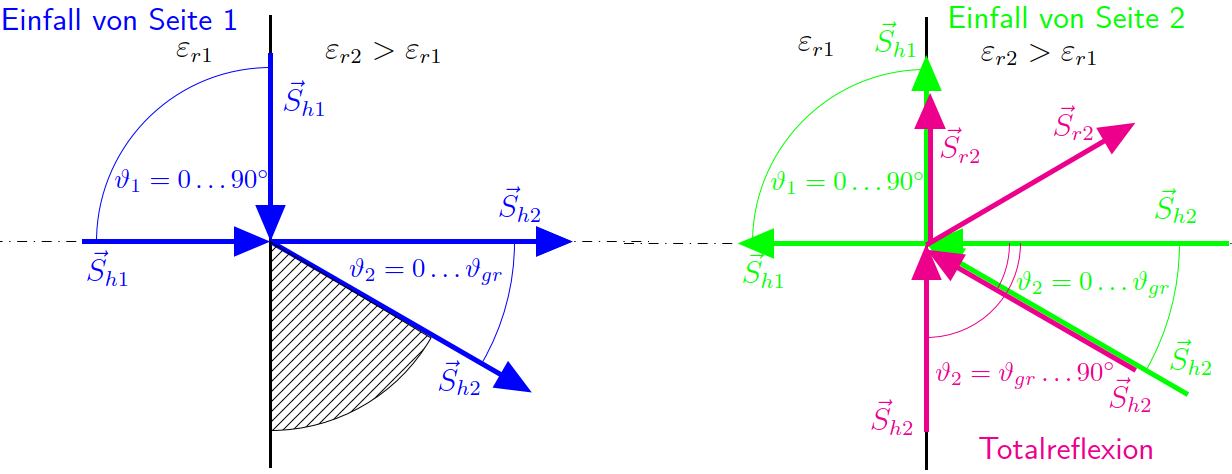
\includegraphics[width=\columnwidth]{Figures/Grenzwinkel_Bild.png}

\subsubsection[Brewster-/Polarisationswinkel]{Brewster-/Polarisationswinkel}
Bei Brewster-Winkel $ \theta_b $ wird Reflexionsfaktor $r=0$.
\begin{itemize}
	%    \item Snelliusche Brechungsgesetz
	%\item Grenzwinkel $\alpha_g$
	% \item[--] Brewsterwinkel $\alpha_B$ (Welle transmittiert reflexionsfrei)
	%       \begin{itemize}
		%           \item[\textbullet] Parallele Polarisation (Nur wenn $\mu_{r1} = \mu_{r2}$)
		%           \item[\textbullet] Senkrechte Polarisation (Nur wenn $\varepsilon_{r1} = \varepsilon_{r2}$)
		%       \end{itemize}
	\item \textbf{Parallele} Polarisation: \quad rechts:
	$ \mu_{r1}=\mu_{r2} $
	\begin{align*}
%		\Aboxed{\mu_{r1}=\mu_{r2}}\\
		\sin\theta_b & = \sqrt{\frac{\varepsilon_2(\mu_2\varepsilon_1 - \mu_1\varepsilon_2)}{\mu_1(\varepsilon_1^2-\varepsilon_2^2)}} &
		\Aboxed{\tan\theta_b & = \sqrt{\frac{\varepsilon_2}{\varepsilon_1}} = \frac{n_2}{n_1}}&
	\end{align*}
		Brewster-Winkel existiert nur bei $ \varepsilon_{r1} \neq \varepsilon_{r2} $.
    \item \textbf{Senkrechte} Polarisation:  \quad rechts: $ \varepsilon_{r1} = \varepsilon_{r2} $
	\begin{align*}
%		\Aboxed{\varepsilon_{r1}=\varepsilon_{r2}}         \\
		\sin\theta_b & = \sqrt{\frac{\mu_2(\mu_2\varepsilon_1 - \mu_1\varepsilon_2)}{\varepsilon_1(\mu_2^2-\mu_1^2)}}&
		\tan\theta_b & = \sqrt{\frac{\mu_2}{\mu_1+\mu_2}}&
	\end{align*}
	Brewster-Winkel existiert nur bei $ \mu_{r1} \neq \mu_{r2} $.\\
	Bei $ \mu_{r1}=\mu_{r2} \rightarrow r \neq 0$ keine Reflexionsfreiheit!
\end{itemize}

\newpage
\subsection{Senkrechte (E-Feld) Polarisation (H-Feld parallel)}
\begin{center}
\begin{tikzpicture}
	\tikzset{cross/.style={cross out, draw=black, minimum size=2*(#1-\pgflinewidth), inner sep=0pt, outer sep=0pt},
		%     %default radius will be 1pt. 
		cross/.default={3.5pt}}
	%Kreuz
	\draw[dotted] (-3,0) -- (3,0);
	\draw[-] (0,2.5) -- (0,-2.5)                
	node[above right]   {$\varepsilon_{r2}, \mu_{r2}, \kappa_{r2}$}
	node[above left]    {$\varepsilon_{r1}, \mu_{r1}, \kappa_{r1}$};
	%Rücklaufende
	\draw[-latex] (-1.5,1) -- (-2.25,1.5)   node[right, yshift=.5ex]{$S_r$};
	\draw[-latex] (-1.5,1) -- (-1,1.75)     node[below, xshift=1ex] {$H_r$};
	\draw[-] (-1.5,1) circle (0.15)         node[below,yshift=-.5ex]{$E_r$};
	\draw[-,fill=black!100] (-1.5,1) circle (0.05);
	\draw[dotted] (-3,2) -- (0,0);
	\draw[latex-latex] (146:1) arc (146:180:1) 
	node[midway, right, yshift=-.7ex] {$\theta_r$};
	
	%Hinlaufende
	\draw[-latex] (-1.5,-1) -- (0,0)        node[below, midway]         {$S_h$};
	\draw[-latex] (-1.5,-1) -- (-1,-1.75)   node[left]                  {$H_h$};
	\draw[-] (-1.5,-1) circle (0.15)        node[above, yshift=.5ex]    {$E_h$};
	\draw[-,fill=black!100] (-1.5,-1) circle (0.05);
	\draw[dotted] (-3,-2) -- (0,0);
	\draw[latex-latex] (180:1) arc (180:214:1)
	node[midway, right, yshift=.7ex] {$\theta_h$};
	
	%Transmitierte
	\draw[-latex] (2,0.6666) -- (3,1)           node[right] {$S_t$};
	\draw[-latex] (2,0.6666) -- (2.2223,0.0448) node[right] {$H_t$};
	\draw[-] (2,0.6666) circle (0.15)           node[above, yshift=.5ex] {$E_t$};
	\draw[-,fill=black!100] (2,0.6666) circle (0.05);
	\draw[dotted] (0,0) -- (3,1);
	\draw[latex-latex] (0:1.5) arc (0:18:1.5)
	node[midway, left, yshift=-.3ex] {$\theta_t$};
	
\end{tikzpicture}
\end{center}



\[ \boxed{\texttt{mit } Z_{F0} = 120\pi \approx 377\si{\ohm}} \]
\begin{align*}
    Z_{Fn}                & = Z_{F0}\cdot\frac{1}{\sqrt{\varepsilon_{rn}}}            \\
    \frac{Z_{F1}}{Z_{F2}} & = \frac{\sqrt{\varepsilon_{r2}}}{\sqrt{\varepsilon_{r1}}}
\end{align*}
\[ n: \texttt{Brechungsindex} \quad ; \quad \theta_h = \theta_r\]
\begin{align*}
    \frac{\sin\theta_t}{\sin\theta_h} & = \frac{\lambda_2}{\lambda_1}= \frac{\beta_1}{\beta_2}= \frac{n_1}{n_2} \\
    \sin\theta_t                      & = \sqrt{\frac{\varepsilon_{r1}}{\varepsilon_{r2}}}\cdot \sin\theta_h
\end{align*}

\begin{itemize}
    \item magnetischer/elektrischer Reflexionsfaktor $[1]$
    \item magnetischer Transmissionsfaktor $[1]$
    \item elektrischer Transmissionsfaktor $[1]$
\end{itemize}
\begin{align*}
    r_s    & =  r_{es} = r_{ms} =                                                                                                                                            \\
           & = \frac{Z_{F2} \cdot \cos \theta_h-Z_{F1} \cdot \cos \theta_t}{Z_{F2} \cdot \cos \theta_h+Z_{F1} \cdot \cos \theta_t}                                           \\
           & = \frac{\cos\theta_h-\sqrt{^{\varepsilon_{r2}}/_{\varepsilon_{r1}}-\sin^2\theta_h}}{\cos\theta_h+\sqrt{^{\varepsilon_{r2}}/_{\varepsilon_{r1}}-\sin^2\theta_h}} \\
    t_{ms} & = Z_{F1} \cdot \frac{2 \cdot \cos \theta_h}{Z_{F2} \cdot \cos \theta_h+Z_{F1} \cdot \cos \theta_t}                                                              \\
           & = (1 - r_s) \cdot \dfrac{\cos \theta_h}{\cos \theta_t}                                                                                                          \\
           & = \frac{Z_{F1}}{Z_{F2}}\cdot t_{es}                                                                                                                             \\
    t_{es} & = Z_{F2} \cdot \frac{2 \cdot \cos \theta_h}{Z_{F2} \cdot \cos \theta_h+Z_{F1} \cdot \cos \theta_t}                                                              \\
           & = 1+r_s
\end{align*}

\begin{align*}
    E_r & = r_s \cdot E_h    \\
    E_t & = t_{es} \cdot E_h \\
    H_r & = r_s \cdot H_h    \\
    H_t & = t_{ms} \cdot H_h \\
    E_t & = H_t\cdot Z_{F2}  \\
    E_h & = H_h\cdot Z_{F1}
\end{align*}

\subsection{Parallel (E-Feld) Polarisation (H-Feld senkrecht)}
\begin{tikzpicture}
    \tikzset{cross/.style={cross out, draw=black, minimum size=2*(#1-\pgflinewidth), inner sep=0pt, outer sep=0pt},
        %     %default radius will be 1pt. 
        cross/.default={3.5pt}}
    %Kreunz
    \draw[dotted] (-3,0) -- (3,0);
    \draw[-] (0, 2.5) -- (0,-2.5) node[above right] {$\varepsilon_{r2}, \mu_{r2}, \kappa_{r2}$}
        node[above left] {$\varepsilon_{r1}, \mu_{r1}, \kappa_{r1}$};
 
    %Hinlaufende
    \draw[-latex] (-1.5,-1) -- (0,0) node[below, midway ]       {$S_h$};
    \draw[-latex] (-1.5,-1) -- (-2,-0.25) node[left, midway]    {$E_h$};
    \draw[-] (-1.5,-1) circle (0.15) node[below,yshift=-.5ex]   {$H_h$};
    \draw[-,fill=black!100] (-1.5,-1) circle (0.05);
    \draw[dotted] (-3,-2) -- (0,0);
    \draw[latex-latex] (180:1) arc (180:214:1)
        node[midway, right, yshift=.7ex] {$\theta_h$};

    %Rücklaufende
    \draw[-latex] (-1.5,1) -- (-2.25,1.5) node[right, yshift=.5ex]          {$S_r$};
    \draw[-latex] (-1.5,1) -- (-2,0.25) node[left, yshift=1ex, xshift=1ex]  {$E_r$};
    \draw[-] (-1.5,1) circle (0.15) node[above, yshift=.5ex]                {$H_r$};
    \draw[-,fill=black!100] (-1.5,1) circle (0.05);
    \draw[dotted] (-3,2) -- (0,0);
    \draw[latex-latex] (146:1) arc (146:180:1)
        node[midway, right, yshift=-.7ex] {$\theta_r$};
        
%    Rücklaufende Sattler
	%    Rücklaufende Sattler
	\draw[-] (-0.8,1.2) circle (0.15) node[right, xshift=.5ex]                {$H_r$};
	\draw(-0.8,1.2) node [cross] {};
 	\draw[-latex] (-0.8,1.2) -- (-0.3,1.95) node[left, yshift=1ex, xshift=1ex]  {$E_r$};
  	\draw[-latex] (-0.8,1.2) -- (-1.55,1.7) node[right, yshift=.5ex]          {$S_r$};

    %Transmitierte
    \draw[-latex] (2,0.6666) -- (3,1) node[right]                   {$S_t$};
    \draw[-latex] (2,0.6666) -- (1.7777,1.378)  node[right]         {$E_t$};
    \draw[-] (2,0.6666) circle (0.15) node[below, yshift=-0.5ex]    {$H_t$};
    \draw[-,fill=black!100] (2,0.6666) circle (0.05);
    \draw[dotted] (0,0) -- (3,1);
    \draw[latex-latex] (0:1.5) arc (0:18:1.5)
        node[midway, left, yshift=-.7] {$\theta_t$};

\end{tikzpicture}

\[ \boxed{\texttt{mit } Z_{F0} = 120\pi \approx 377\si{\ohm}} \]
\begin{align*}
    Z_{Fn}                & = Z_{F0}\cdot\frac{1}{\sqrt{\varepsilon_{rn}}}            \\
    \frac{Z_{F1}}{Z_{F2}} & = \frac{\sqrt{\varepsilon_{r2}}}{\sqrt{\varepsilon_{r1}}}
\end{align*}
\[ n: \texttt{Brechungsindex} \quad ; \quad \theta_h = \theta_r\]
\begin{align*}
    \frac{\sin\theta_t}{\sin\theta_h} & = \frac{\lambda_2}{\lambda_1}= \frac{\beta_1}{\beta_2}= \frac{n_1}{n_2} \\
    \sin\theta_t                      & = \sqrt{\frac{\varepsilon_{r1}}{\varepsilon_{r2}}}\cdot\sin\theta_h
\end{align*}

\begin{itemize}
    \item magnetischer/elektrischer Reflexionsfaktor $[1]$
    \item magnetischer Transmissionsfaktor $[1]$
    \item elektrischer Transmissionsfaktor $[1]$
\end{itemize}
\begin{align*}
    r_p    & =  r_{ep} = r_{mp} =                                                                                                                                                                                                        \\
           & = \frac{Z_{F2} \cdot \cos \theta_t-Z_{F1} \cdot \cos \theta_h}{Z_{F2} \cdot \cos \theta_t+Z_{F1} \cdot \cos \theta_h} =                                                                                                     \\
           & = \frac{\varepsilon_{r2}\cos\theta_h-\sqrt{\varepsilon_{r2}\varepsilon_{r1}-{\varepsilon_{r1}}^2\sin^2\theta_h}}{\varepsilon_{r2}\cos\theta_h+\sqrt{{\varepsilon_{r2}\varepsilon_{r1}-{\varepsilon_{r1}}^2\sin^2\theta_h}}} \\
    t_{mp} & = Z_{F1} \cdot \frac{2 \cdot \cos \theta_h}{Z_{F1} \cdot \cos \theta_h+Z_{F2} \cdot \cos \theta_t}                                                                                                                          \\
           & = 1+r_p                                                                                                                                                                                                                     \\
    t_{ep} & = Z_{F2} \cdot \frac{2 \cdot \cos \theta_h}{Z_{F1} \cdot \cos \theta_h+Z_{F2} \cdot \cos \theta_t}                                                                                                                          \\
           & = (1-r_p) \cdot \dfrac{\cos \theta_h}{\cos \theta_t}                                                                                                                                                                        \\
           & = \frac{Z_{F2}}{Z_{F1}}\cdot t_{mp}
\end{align*}

\begin{align*}
    E_r & = r_p\cdot E_h    \\
    E_t & = t_{ep}\cdot E_h \\
    H_r & = r_p\cdot H_h    \\
    H_t & = t_{mp}\cdot H_h \\
    E_t & = H_t\cdot Z_{F2} \\
    E_h & = H_h\cdot Z_{F1}
\end{align*}

\newpage
\subsubsection{Senkrechte Polarisation mit $\mu_r$}
\begin{center}
\begin{tikzpicture}
	\tikzset{cross/.style={cross out, draw=black, minimum size=2*(#1-\pgflinewidth), inner sep=0pt, outer sep=0pt},
		%     %default radius will be 1pt. 
		cross/.default={3.5pt}}
	%Kreuz
	\draw[dotted] (-3,0) -- (3,0);
	\draw[-] (0,2.5) -- (0,-2.5)                
	node[above right]   {$\varepsilon_{r2}, \mu_{r2}, \kappa_{r2}$}
	node[above left]    {$\varepsilon_{r1}, \mu_{r1}, \kappa_{r1}$};
	%Rücklaufende
	\draw[-latex] (-1.5,1) -- (-2.25,1.5)   node[right, yshift=.5ex]{$S_r$};
	\draw[-latex] (-1.5,1) -- (-1,1.75)     node[below, xshift=1ex] {$H_r$};
	\draw[-] (-1.5,1) circle (0.15)         node[below,yshift=-.5ex]{$E_r$};
	\draw[-,fill=black!100] (-1.5,1) circle (0.05);
	\draw[dotted] (-3,2) -- (0,0);
	\draw[latex-latex] (146:1) arc (146:180:1) 
	node[midway, right, yshift=-.7ex] {$\theta_r$};
	
	%Hinlaufende
	\draw[-latex] (-1.5,-1) -- (0,0)        node[below, midway]         {$S_h$};
	\draw[-latex] (-1.5,-1) -- (-1,-1.75)   node[left]                  {$H_h$};
	\draw[-] (-1.5,-1) circle (0.15)        node[above, yshift=.5ex]    {$E_h$};
	\draw[-,fill=black!100] (-1.5,-1) circle (0.05);
	\draw[dotted] (-3,-2) -- (0,0);
	\draw[latex-latex] (180:1) arc (180:214:1)
	node[midway, right, yshift=.7ex] {$\theta_h$};
	
	%Transmitierte
	\draw[-latex] (2,0.6666) -- (3,1)           node[right] {$S_t$};
	\draw[-latex] (2,0.6666) -- (2.2223,0.0448) node[right] {$H_t$};
	\draw[-] (2,0.6666) circle (0.15)           node[above, yshift=.5ex] {$E_t$};
	\draw[-,fill=black!100] (2,0.6666) circle (0.05);
	\draw[dotted] (0,0) -- (3,1);
	\draw[latex-latex] (0:1.5) arc (0:18:1.5)
	node[midway, left, yshift=-.3ex] {$\theta_t$};
	
\end{tikzpicture}
\end{center}


$\vec{E}$-Feld senkrecht, $ \vec{H}$-Feld parallel. \qquad $ \mu_{r1} \neq \mu_{r2} $
%\[ \boxed{\texttt{mit } Z_{F0} = 120\pi \approx 377\si{\ohm}} \]
\begin{flalign*}
	Z_{F0} &= 120\pi \,\si{\ohm} &
	Z_{F(n)}                & = Z_{F0}\cdot\sqrt{\frac{\mu_{r(n)}}{\varepsilon_{r(n)}}}&
	\frac{Z_{F1}}{Z_{F2}} & = \frac{\sqrt{\mu_{r 1}\varepsilon_{r2}}}{\sqrt{\mu_{r 2}\varepsilon_{r1}}}&
\end{flalign*}
%\[ n: \texttt{Brechungsindex} \quad ; \quad \theta_h = \theta_r\]
\textbf{Brechungsgesetz}: \qquad  mit $ \theta_h = \theta_r\ $
\begin{flalign*}
	\Aboxed{\frac{\sin\theta_t}{\sin\theta_h} & = \sqrt{\frac{\mu_{r 1}\varepsilon_{r1}}{\mu_{r 2}\varepsilon_{r2}}}} = \frac{\lambda_2}{\lambda_1}= \frac{\beta_1}{\beta_2}= \frac{n_1}{n_2} &
%	\sin\theta_t                      & = \sqrt{\frac{\varepsilon_{r1}}{\varepsilon_{r2}}}\cdot \sin\theta_h 
\end{flalign*}
%\begin{align*}
%	\dfrac{\sin \vartheta_{2}}{\sin \vartheta_{1}} = \dfrac{k_{h}}{k_{g}} & = \sqrt{\dfrac{\mu_{r 1} \varepsilon_{r 1}}{\mu_{r 2} \varepsilon_{r 2}}} = \dfrac{n_{1}}{n_{2}} = \dfrac{v_{p, 2}}{v_{p, 1}} = \dfrac{\lambda_{2}}{\lambda_{1}} \\
%	% \alpha_{Bp}                                                           & = \tan^{-1} \left( \sqrt{ \dfrac{\varepsilon_{r1}}{\varepsilon_{r2}}} \right)                                                                                        \\
%	% \alpha_{Bs}                                                           & = \tan^{-1} \left( \sqrt{ \dfrac{\mu_{r1}}{\mu_{r2}}} \right)
%\end{align*}


%\begin{itemize}
%    \item magnetischer/elektrischer Reflexionsfaktor $[1]$
%    \item magnetischer Transmissionsfaktor $[1]$
%    \item elektrischer Transmissionsfaktor $[1]$
%\end{itemize}
\textbf{Fresnelsche Formeln}: \qquad $ \theta_h = \vartheta_{1} $ \quad $ \theta_t = \vartheta_{2} $
\begin{equation*}
	\setlength{\jot}{10pt}
	\begin{aligned}
		r_s    & =  r_{es} = r_{ms} =                                                                                                                                            \\
		& = \frac{Z_{F2} \cdot \cos \theta_h-Z_{F1} \cdot \cos \theta_t}{Z_{F2} \cdot \cos \theta_h+Z_{F1} \cdot \cos \theta_t}                                           \\
		%		& = \frac{\cos\theta_h-\sqrt{^{\varepsilon_{r2}}/_{\varepsilon_{r1}}-\sin^2\theta_h}}{\cos\theta_h+\sqrt{^{\varepsilon_{r2}}/_{\varepsilon_{r1}}-\sin^2\theta_h}} \\
& =\frac{\cos \vartheta_1-\sqrt{\frac{\mu_{r 1} \varepsilon_{r 2}}{\mu_{r 2} \varepsilon_{r 1}}-\frac{\mu_{r 1}{ }^2}{\mu_{r 2}^2} \sin ^2 \vartheta_1}}{\cos \vartheta_1+\sqrt{\frac{\mu_{r 1} \varepsilon_{r 2}}{\mu_{r 2} \varepsilon_{r 1}}-\frac{\mu_{r 1}{ }^2}{\mu_{r 2}^2} \sin ^2 \vartheta_1}} \\
		t_{es} & =\frac{2 \cdot	 Z_{F2} \cdot \cos \theta_h}{Z_{F2} \cdot \cos \theta_h+Z_{F1} \cdot \cos \theta_t}                                                              \\
& =\frac{2 \cos \vartheta_1}{\cos \vartheta_1+\sqrt{\frac{\mu_{r 1} \varepsilon_{r 2}}{\mu_{r 2} \varepsilon_{r 1}}-\frac{\mu_{r 1}{ }^2}{\mu_{r 2}{ }^2} \sin ^2 \vartheta_1}} \\
		& = 1+r_s\\
		t_{ms} & = \frac{2 Z_{F1} \cdot \cos \theta_h}{Z_{F2} \cdot \cos \theta_h+Z_{F1} \cdot \cos \theta_t}                                                              \\
		& =\frac{2 \sqrt{\frac{\mu_{r 1} \varepsilon_{r 2}}{\mu_{r 2} \varepsilon_{r 1}}} \cos \vartheta_1}{\cos \vartheta_1+\sqrt{\frac{\mu_{r 1} \varepsilon_{r 2}}{\mu_{r 2} \varepsilon_{r 1}}-\frac{\mu_{r 1}{ }^2}{\mu_{r 2}{ }^2} \sin ^2 \vartheta_1}}
		\\
%		& = (1 - r_s) \cdot \dfrac{\cos \theta_h}{\cos \theta_t}                                                                                                          \\
		& = \frac{Z_{F1}}{Z_{F2}}\cdot t_{es}\\
		& =\sqrt{\frac{\mu_{r 1} \varepsilon_{r 2}}{\mu_{r 2} \varepsilon_{r 1}}} t_{e s}                                                                                                                   
	\end{aligned}
\end{equation*}


%\begin{align*}
%    r_s    & =  r_{es} = r_{ms} =                                                                                                                                            \\
%           & = \frac{Z_{F2} \cdot \cos \theta_h-Z_{F1} \cdot \cos \theta_t}{Z_{F2} \cdot \cos \theta_h+Z_{F1} \cdot \cos \theta_t}                                           \\
%           & = \frac{\cos\theta_h-\sqrt{^{\varepsilon_{r2}}/_{\varepsilon_{r1}}-\sin^2\theta_h}}{\cos\theta_h+\sqrt{^{\varepsilon_{r2}}/_{\varepsilon_{r1}}-\sin^2\theta_h}} \\
%           & = \frac{\sqrt{\varepsilon_{r1}}\cdot\cos\theta_h - \sqrt{\varepsilon_{r2}}\cdot\cos\theta_t}{\sqrt{\varepsilon_{r2}}\cdot\cos\theta_t + \sqrt{\varepsilon_{r1}}\cos\theta_h} \\
%    t_{ms} & = Z_{F1} \cdot \frac{2 \cdot \cos \theta_h}{Z_{F2} \cdot \cos \theta_h+Z_{F1} \cdot \cos \theta_t}                                                              \\
%           & = (1 - r_s) \cdot \dfrac{\cos \theta_h}{\cos \theta_t}                                                                                                          \\
%           & = \frac{Z_{F1}}{Z_{F2}}\cdot t_{es}                                                                                                                             \\
%    t_{es} & = Z_{F2} \cdot \frac{2 \cdot \cos \theta_h}{Z_{F2} \cdot \cos \theta_h+Z_{F1} \cdot \cos \theta_t}                                                              \\
%           & = 1+r_s
%\end{align*}
%\subsubsection*{Beziehungen Polarisation}
%\textbf{Beziehungen Polarisation}
%\begin{equation*}
%	\begin{aligned}
%		E_r & = r_s \cdot E_h    \\
%		E_t & = t_{es} \cdot E_h \\
%		H_r & = r_s \cdot H_h    \\
%		H_t & = t_{ms} \cdot H_h \\
%		E_t & = H_t\cdot Z_{F2}  \\
%		E_h & = H_h\cdot Z_{F1}
%	\end{aligned}
%	\qquad
%	\begin{aligned}
%		E_r & = r_p\cdot E_h    \\
%		E_t & = t_{ep}\cdot E_h \\
%		H_r & = r_p\cdot H_h    \\
%		H_t & = t_{mp}\cdot H_h \\
%		E_t & = H_t\cdot Z_{F2} \\
%		E_h & = H_h\cdot Z_{F1} 
%	\end{aligned}
%\end{equation*}
%
%\textbf{Richtungssinn Felder (Hand-Regel)}
%\begin{equation*}
%	\begin{aligned}
%		& \text{\textbf{Linke Hand}}\\
%		& \text{Daumen:}\quad \vec{E}\\
%		& \text{Zeigef.:}\quad \vec{S}_{av}\\
%		& \text{Mittelf.:}\quad \vec{H} 
%	\end{aligned}
%	\qquad
%	\begin{aligned}
%		& \text{\textbf{Rechte Hand}}\\
%		& \text{Daumen:}\quad \vec{E}\\
%		& \text{Zeigef.:}\quad \vec{H}\\
%		& \text{Mittelf.:}\quad \vec{S}_{av}
%	\end{aligned}
%\end{equation*}
\newcolumn
\subsubsection{Parallele Polarisation mit $\mu_r$}
\begin{center}
	\begin{tikzpicture}
    \tikzset{cross/.style={cross out, draw=black, minimum size=2*(#1-\pgflinewidth), inner sep=0pt, outer sep=0pt},
        %     %default radius will be 1pt. 
        cross/.default={3.5pt}}
    %Kreunz
    \draw[dotted] (-3,0) -- (3,0);
    \draw[-] (0, 2.5) -- (0,-2.5) node[above right] {$\varepsilon_{r2}, \mu_{r2}, \kappa_{r2}$}
        node[above left] {$\varepsilon_{r1}, \mu_{r1}, \kappa_{r1}$};
 
    %Hinlaufende
    \draw[-latex] (-1.5,-1) -- (0,0) node[below, midway ]       {$S_h$};
    \draw[-latex] (-1.5,-1) -- (-2,-0.25) node[left, midway]    {$E_h$};
    \draw[-] (-1.5,-1) circle (0.15) node[below,yshift=-.5ex]   {$H_h$};
    \draw[-,fill=black!100] (-1.5,-1) circle (0.05);
    \draw[dotted] (-3,-2) -- (0,0);
    \draw[latex-latex] (180:1) arc (180:214:1)
        node[midway, right, yshift=.7ex] {$\theta_h$};

    %Rücklaufende
    \draw[-latex] (-1.5,1) -- (-2.25,1.5) node[right, yshift=.5ex]          {$S_r$};
    \draw[-latex] (-1.5,1) -- (-2,0.25) node[left, yshift=1ex, xshift=1ex]  {$E_r$};
    \draw[-] (-1.5,1) circle (0.15) node[above, yshift=.5ex]                {$H_r$};
    \draw[-,fill=black!100] (-1.5,1) circle (0.05);
    \draw[dotted] (-3,2) -- (0,0);
    \draw[latex-latex] (146:1) arc (146:180:1)
        node[midway, right, yshift=-.7ex] {$\theta_r$};
        
%    Rücklaufende Sattler
	%    Rücklaufende Sattler
	\draw[-] (-0.8,1.2) circle (0.15) node[right, xshift=.5ex]                {$H_r$};
	\draw(-0.8,1.2) node [cross] {};
 	\draw[-latex] (-0.8,1.2) -- (-0.3,1.95) node[left, yshift=1ex, xshift=1ex]  {$E_r$};
  	\draw[-latex] (-0.8,1.2) -- (-1.55,1.7) node[right, yshift=.5ex]          {$S_r$};

    %Transmitierte
    \draw[-latex] (2,0.6666) -- (3,1) node[right]                   {$S_t$};
    \draw[-latex] (2,0.6666) -- (1.7777,1.378)  node[right]         {$E_t$};
    \draw[-] (2,0.6666) circle (0.15) node[below, yshift=-0.5ex]    {$H_t$};
    \draw[-,fill=black!100] (2,0.6666) circle (0.05);
    \draw[dotted] (0,0) -- (3,1);
    \draw[latex-latex] (0:1.5) arc (0:18:1.5)
        node[midway, left, yshift=-.7] {$\theta_t$};

\end{tikzpicture}
\end{center}
$\vec{E}$-Feld parallel, $ \vec{H}$-Feld senkrecht. \qquad $ \mu_{r1} \neq \mu_{r2} $\\

Stücke: $\vec{H}_h$ und $ \vec{H}_r$ zeigen in die selbe Richtung!\\
Sattler: $\vec{H}_h$ und $ \vec{H}_r$ zeigen in \textbf{entgegengesetzter} Richtung!\\
%\[ \boxed{\texttt{mit } Z_{F0} = 120\pi \approx 377\si{\ohm}} \]
%\begin{align*}
%    Z_{Fn}                & = Z_{F0}\cdot\frac{1}{\sqrt{\varepsilon_{rn}}}            \\
%    \frac{Z_{F1}}{Z_{F2}} & = \frac{\sqrt{\varepsilon_{r2}}}{\sqrt{\varepsilon_{r1}}}
%\end{align*}
%\[ n: \texttt{Brechungsindex} \quad ; \quad \theta_h = \theta_r\]
%\begin{align*}
%    \frac{\sin\theta_t}{\sin\theta_h} & = \frac{\lambda_2}{\lambda_1}= \frac{\beta_1}{\beta_2}= \frac{n_1}{n_2} \\
%    \sin\theta_t                      & = \sqrt{\frac{\varepsilon_{r1}}{\varepsilon_{r2}}}\cdot\sin\theta_h
%\end{align*}

%\begin{itemize}
%    \item magnetischer/elektrischer Reflexionsfaktor $[1]$
%    \item magnetischer Transmissionsfaktor $[1]$
%    \item elektrischer Transmissionsfaktor $[1]$
%\end{itemize}
\textbf{Fresnelsche Formeln (Stücke)}: \qquad $ \theta_h = \vartheta_{1} $ \quad $ \theta_t = \vartheta_{2} $
\begin{equation*}
	\setlength{\jot}{10pt}
	\begin{aligned}
		r_{ep}    & =  r_{mp} = r_{p}  \qquad \qquad =-r_{p,[\texttt{Sattler}]}
		\\
		& = \frac{Z_{F1} \cdot \cos \theta_h-Z_{F2} \cdot \cos \theta_t}{Z_{F1} \cdot \cos \theta_h+Z_{F2} \cdot \cos \theta_t}
		\\
		%		& = - \left( \frac{\varepsilon_{r2}\cos\theta_h-\sqrt{\varepsilon_{r2}\varepsilon_{r1}-{\varepsilon_{r1}}^2\sin^2\theta_h}}{\varepsilon_{r2}\cos\theta_h+\sqrt{{\varepsilon_{r2}\varepsilon_{r1}-{\varepsilon_{r1}}^2\sin^2\theta_h}}} \right)  
		%		\\
%		& =\frac{\cos \vartheta_1-\sqrt{\frac{\varepsilon_{r 1}}{\varepsilon_{r 2}}-\frac{\varepsilon_{r 1}{ }^2}{\varepsilon_{r 2}{ }^2} \sin ^2 \vartheta_1}}{\cos \vartheta_1+\sqrt{\frac{\varepsilon_{r 1}}{\varepsilon_{r 2}}-\frac{\varepsilon_{r 1}{ }^2}{\varepsilon_{r 2}{ }^2} \sin ^2 \vartheta_1}}
%		\\
		& =\frac{\cos \vartheta_1-\sqrt{\frac{\mu_{r 2} \varepsilon_{r 1}}{\mu_{r 1} \varepsilon_{r 2}}-\frac{\varepsilon_{r 1}{ }^2}{\varepsilon_{r 2}{ }^2} \sin ^2 \vartheta_1}}{\cos \vartheta_1+\sqrt{\frac{\mu_{r 2} \varepsilon_{r 1}}{\mu_{r 1} \varepsilon_{r 2}}-\frac{\varepsilon_{r 1}{ }^2}{\varepsilon_{r 2}{} ^2} \sin ^2 \vartheta_1}} \\
		t_{ep} & =  \frac{2 \cdot Z_{F2}   \cdot  \cos \theta_h}{Z_{F1} \cdot \cos \theta_h+Z_{F2} \cdot \cos \theta_t}\\                                                                                                                           %= (1-r_p) \cdot \dfrac{\cos \theta_h}{\cos \theta_t}                                                                                                                                                                        \\
				&=\frac{2 \sqrt{\frac{\mu_{r 2} \varepsilon_{r 1}}{\mu_{r 1} \varepsilon_{r 2}}} \cos \vartheta_1}{\cos \vartheta_1+\sqrt{\frac{\mu_{r 2} \varepsilon_{r 1}}{\mu_{r 1} \varepsilon_{r 2}}-\frac{\varepsilon_{r 1}{ }^2}{\varepsilon_{r 2}{ }^2} \sin ^2 \vartheta_1}} \\
%		& = \frac{2 \sqrt{\frac{\varepsilon_{r 1}}{\varepsilon_{r 2}}} \cos \vartheta_1}{\cos \vartheta_1+\sqrt{\frac{\varepsilon_{r 1}}{\varepsilon_{r 2}}-\frac{\varepsilon_{r 1}^2}{\varepsilon_{r 2}{ }^2} \sin ^2 \vartheta_1}}
%		\\
		& = \frac{Z_{F2}}{Z_{F1}}\cdot t_{mp} = \sqrt{\frac{\mu_{r2}\varepsilon_{r1}}{\mu_{r1}\varepsilon_{r2}}}\cdot t_{mp} 
		\\
		t_{mp} & = \frac{2 \cdot  Z_{F1}\cdot \cos \theta_h}{Z_{F1} \cdot \cos \theta_h+Z_{F2} \cdot \cos \theta_t}                    
\\
		&=\frac{2 \cos \vartheta_1}{\cos \vartheta_1+\sqrt{\frac{\mu_{r 2} \varepsilon_{r 1}}{\mu_{r 1} \varepsilon_{r 2}}-\frac{\varepsilon_{r 1}{ }^2}{\varepsilon_{r 2}{ }^2} \sin ^2 \vartheta_1}}   \\
		&		= 1+r_p
	\end{aligned}
\end{equation*}
%\begin{align*}
%    r_p    & =  r_{ep} = r_{mp} =                                                                                                                                                                                                        \\
%           & = \frac{Z_{F1} \cdot \cos \theta_t-Z_{F2} \cdot \cos \theta_h}{Z_{F2} \cdot \cos \theta_t+Z_{F1} \cdot \cos \theta_h} =                                                                                                     \\
%           & = \frac{\varepsilon_{r2}\cos\theta_h-\sqrt{\varepsilon_{r2}\varepsilon_{r1}-{\varepsilon_{r1}}^2\sin^2\theta_h}}{\varepsilon_{r2}\cos\theta_h+\sqrt{{\varepsilon_{r2}\varepsilon_{r1}-{\varepsilon_{r1}}^2\sin^2\theta_h}}} \\
%               t_{ep} & = Z_{F2} \cdot \frac{2 \cdot \cos \theta_h}{Z_{F1} \cdot \cos \theta_h+Z_{F2} \cdot \cos \theta_t}                                                                                                                          \\
%           & = (1-r_p) \cdot \dfrac{\cos \theta_h}{\cos \theta_t}                                                                                                                                                                        \\
%           & = \frac{Z_{F2}}{Z_{F1}}\cdot t_{mp}\\
%    t_{mp} & = \frac{2 Z_{F1}\cdot \cos \theta_h}{Z_{F1} \cdot \cos \theta_h+Z_{F2} \cdot \cos \theta_t}                                                                                                                          \\
%           & = 1+r_p                                                                                                                                                                                                                
%\end{align*}
%\textbf{Fresnelsche Formeln (Sattler)}:
%\begin{equation*}
%	\setlength{\jot}{10pt}
%	\begin{aligned}
%		r_p    & =  r_{ep} = r_{mp} \qquad \qquad =-r_{p,[\texttt{Stücke}]}                                                    \\
%		& = \frac{Z_{F2} \cdot \cos \theta_t-Z_{F1} \cdot \cos \theta_h}{Z_{F2} \cdot \cos \theta_t+Z_{F1} \cdot \cos \theta_h}                                                                                               \\
%		& = \frac{\sqrt{\varepsilon_{r1}}\cdot\cos\theta_t - \sqrt{\varepsilon_{r2}}\cdot\cos\theta_h}{\sqrt{\varepsilon_{r2}}\cdot\cos\theta_h + \sqrt{\varepsilon_{r1}}\cos\theta_t} \\
%		t_{ep} & =  \frac{2 Z_{F2} \cdot \cos \theta_h}{Z_{F1} \cdot \cos \theta_h+Z_{F2} \cdot \cos \theta_t}                                                                                                                          \\
%		& = \frac{2\cdot\sqrt{\varepsilon_{r1}}\cdot\cos\theta_h}{\sqrt{\varepsilon_{r2}}\cdot\cos\theta_h + \sqrt{\varepsilon_{r1}}\cdot\cos\theta_t}\\
%		& = (1+r_p) \cdot \dfrac{\cos \theta_h}{\cos \theta_t}\\
%		t_{mp} 
%		%	& 
%		%	= \frac{2 Z_{F1}\cdot \cos \theta_h}{Z_{F1} \cdot \cos \theta_h+Z_{F2} \cdot \cos \theta_t}                                                                                                                          \\
%		& = 1-r_p                                                                                                                                                                                                                                                                                                                                                                                        = \frac{Z_{F1}}{Z_{F2}}\cdot t_{ep}
%	\end{aligned}
%\end{equation*}


%\begin{align*}
%    E_r & = r_p\cdot E_h    \\
%    E_t & = t_{ep}\cdot E_h \\
%    H_r & = r_p\cdot H_h    \\
%    H_t & = t_{mp}\cdot H_h \\
%    E_t & = H_t\cdot Z_{F2} \\
%    E_h & = H_h\cdot Z_{F1}
%\end{align*}

    \section{Leitungen}
\includegraphics[width=1\columnwidth]{Figures/ZahlentabelleLeitungsparameter.png}

\subsection{Leitungsparameter}

{\small\[
        \sigma = \text{Leitwert des Dielektr.} \qquad \sigma_c = \text{Leitwert des Leiters}
    \]}

\subsubsection{Parallele Platten}
{\small\[
        w  = \text{Platten Breite} \qquad d  = \text{Abstand zw. Platten}
    \]}

Für Sinus-Anregung:
\begin{align*}
    I & = \frac{U}{Z_L} = \underbrace{\frac{U_0}{Z_L}}_{I_0}\cdot e^{-j\beta z\cdot e^{j\omega t}}                         \\
    U & = \int \vec{E} d\vec{s} \stackrel{w\gg d}{=} E\cdot d \rightarrow E = \frac{U_0}{d}\cdot^{-j\beta z}\cdot\vec{e}_x \\
    I & = \oint \vec{H} d\vec{s} =  H\cdot w \rightarrow H = \frac{I_0}{w}\cdot^{-j\beta z}\cdot\vec{e}_y                  % \\
    % \vec{E}(r, z) & = \frac{I}{2\pi r}\cdot Z_F\cdot e^{-j\beta z} \cdot\vec{e}_r                                                      \\
    %               & = \frac{\hat{U}}{r \cdot\ln{(^{2b}/_{2a})}}\cdot e^{-j\beta z}\cdot\vec{e}_r
\end{align*}

\begin{tikzpicture}
    \tikzset{cross/.style={cross out, draw=black, minimum size=2*(#1-\pgflinewidth), inner sep=0pt, outer sep=0pt},
        %     %default radius will be 1pt. 
        cross/.default={3.5pt}}

        %Untereplatte
        \draw[-](0,0)--(0,0.35);
        \draw[-](2,0)--(2,0.35);

        \draw[-](0,0)--(2,0);
        \draw[-](0,0.35)--(2,0.35);

        \draw[-](0,0.35)--(0.3,0.65);
        \draw[-](2,0)--(3,1);
        \draw[-](2,0.35)--(3,1.35);

        \draw[-](1,0.175) circle (0.15);
        \draw[-,fill=black!100] (1,0.175) circle (0.05);

        %Obere Platte
        \draw[-](0,0.65)--(0,1);
        \draw[-](2,0.65)--(2,1);

        \draw[-](0,0.65)--(2,0.65);
        \draw[-](0,1)--(2,1);

        \draw[-](0,1)--(1,2);
        \draw[-](2,1)--(3,2);
        \draw[-](2,0.65)--(3,1.65);

        \draw[-](1,0.825) circle (0.15);
        \draw(1,0.825) node [cross] {};
   
\end{tikzpicture}

{\renewcommand*{\arraystretch}{0.2}
    \begin{tabularx}{0.5\columnwidth}{|X|}
        \hline
        \[R=\frac{2}{w\delta\sigma}\] \\
        \hline
        \[L=\frac{\mu d}{w}\]         \\
        \hline
        \[G=\frac{\sigma w}{d}\]      \\
        \hline
        \[C=\frac{w\varepsilon}{d}\]  \\
        \hline
    \end{tabularx}
}

\subsubsection{Doppelleitung:}
{\small\[
        a = \text{Leiter Radius} \qquad d = \text{Abstand zw. den Leitern}\\
    \]}
{\small\[
        \text{cosh am TR: MENU $\rightarrow$ 1; OPTN $\rightarrow$ 1 $\rightarrow$ 5}\\
    \]}
\begin{tikzpicture}
    \tikzset{cross/.style={cross out, draw=black, minimum size=2*(#1-\pgflinewidth), inner sep=0pt, outer sep=0pt},
        %     %default radius will be 1pt. 
        cross/.default={3.5pt}}

        %linker Außenleiter
        \draw[-](-0.53,0.53)--(0.97,2.03);

        
        \draw[-](48:0.75) arc (48:312:0.75);

        %linker Innenleiter
        \draw[dashed](-0.106,0.106)--(0.41,0.622);
        \draw[dashed](0.106,-0.106)--(0.922,0.71);

        \draw[-](0,0) circle (0.15);
        \draw(0,0) node [cross] {};


        
        %%%%%%%%%%%%%%%%%%%%%%%%%%%%%%%%%%%%%%%%%%%%%%%%%%%%%%%%%%%
        %%%%%%%%%%%%%%%%%%%%%%%%%%%%%%%%%%%%%%%%%%%%%%%%%%%%%%%%%%%

        %Rechter Außenleiter
        \draw[-](0.48,0.58)--(1.97,2.03);
        \draw[-](1.53,-0.53)--(2.13,0.07);
        \draw([shift={(228:0.75)}]1,0) arc (-132:132:0.75);

        %Rechter Innenleiter
        \draw[dashed](0.894,0.106)--(1.41,0.622);
        \draw[dashed](1.106,-0.106)--(1.622,0.41);

        \draw[-](1,0) circle (0.15);
        \draw[-,fill=black!100] (1,0) circle (0.05);

        

\end{tikzpicture}

{\renewcommand*{\arraystretch}{0.2}
    \begin{tabularx}{0.5\columnwidth}{|X|}
        \hline
        \[R  = \frac{1}{\pi a\delta\sigma_c}\]              \\
        \hline
        \[L = \frac{\mu}{\pi} \cosh^{-1}\frac{d}{2a}\]      \\
        \hline
        \[G = \frac{\pi\sigma}{\cosh^{-1}(^d/_{2a})}\]      \\
        \hline
        \[C = \frac{\pi\varepsilon}{\cosh^{-1}(^d/_{2a})}\] \\
        \hline
    \end{tabularx}}

\subsubsection{Koaxial Leitung}
{\small\[
        a = \text{innen Radius} \qquad b = \text{außen Radius} \\
    \]}
\begin{align*}
    \vec{H}(r, z)         & = \frac{\hat{I}}{2\pi r}\cdot e^{-j\beta z}\cdot\vec{e}_\varphi                   \\
    \vec{E}(r, z)         & = \frac{\hat{I}}{2\pi r}\cdot Z_{F0}\cdot e^{-j\beta z} \cdot\vec{e}_r
                          & = \frac{\hat{U}}{r \cdot\ln{(^{b}/_{a})}}\cdot e^{-j\beta z}\cdot\vec{e}_r        \\
    \vec{S}_{zeit.Mittel} & = \frac{1}{2}\cdot\left[\frac{\hat{I}}{2\pi r}\right]^2\cdot Z_{F0}\cdot\vec{e}_z
\end{align*}
\begin{tikzpicture}
    \tikzset{cross/.style={cross out, draw=black, minimum size=2*(#1-\pgflinewidth), inner sep=0pt, outer sep=0pt},
        %     %default radius will be 1pt. 
        cross/.default={3.5pt}}

        %Außenleiter
        \draw[-](-0.53,0.53)--(1.07,2.13);
        \draw[-](0.53,-0.53)--(2.23,1.17);

        \draw[-](0,0) circle (0.75);

        %Innenleiter
        \draw[-](-0.106,0.106)--(0.41,0.622);
        \draw[-](0.106,-0.106)--(0.622,0.41);

        \draw[-](0,0) circle (0.15);
        \draw(0,0) node [cross] {};

\end{tikzpicture}

{\renewcommand*{\arraystretch}{0.2}
    \begin{tabularx}{0.5\columnwidth}{|X|}
        \hline
        \[R=\frac{1}{2\pi\delta\sigma_c}\left[\frac{1}{a}+\frac{1}{b}\right]\] \\
        \hline
        \[L=\frac{\mu}{2\pi}\ln\frac{b}{a}\]                                   \\
        \hline
        \[G=\frac{2\pi\sigma}{\ln(^b/_a)}\]                                    \\
        \hline
        \[C=\frac{2\pi\varepsilon}{\ln(^b/_a)}\]                               \\
        \hline
    \end{tabularx}}



\vspace{1ex}
Für beliebige Leitergeometrie gelten folgende Zusammenhänge:
\[
    LC = \mu\varepsilon \quad \text{und} \quad \frac{G}{C} = \frac{\sigma}{\varepsilon}
\]
Innere Induktivität:
\[
    L_i = \frac{R}{w}
\]
\textbf{\color{red}{Leitungen gehen HIN und ZURÜCK!!!}\\
    \color{red}{Länge verdoppeln!!!}
}
\subsection{Allgemeine Lösung Leitungsgleichung}
\begin{align*}
    \underline{U}(z)   & = U_h e^{\underline{\gamma} z} + U_r e^{-\underline{\gamma} z} = U_h e^{\underline{\gamma} d} + U_r e^{-\underline{\gamma} d}                       \\
    \underline{I}(z)   & = I_h e^{\underline{\gamma} z} + I_r e^{-\underline{\gamma} z} = \frac{U_h}{Z_L}e^{\underline{\gamma} d} - \frac{U_r}{Z_L}e^{-\underline{\gamma} d} \\
    \underline{Z}_L    & = \frac{U_h}{I_h} = \sqrt{ \frac{R + j \omega L}{G + j \omega C}}                                                                                   \\
    \underline{\gamma} & = j \omega \sqrt{LC} \cdot \sqrt{ \frac{RG}{j^2 \omega^2 LC} + \frac{G}{j \omega C} + \frac{R}{j \omega L} + 1}                                     \\
                       & = \sqrt{(R+j\omega L)\cdot(G+j\omega C)}                                                                                                            \\
    \lambda            & = \frac{2 \pi}{\beta}                                                                                                                               \\
    v_p                & = \frac{\omega}{\beta}                                                                                                                              \\
    l_\texttt{elektr.} & = \beta \cdot l                                                                                                                                     \\
    \alpha             & = \omega \cdot \sqrt{\dfrac{\mu \varepsilon}{2}\cdot \left(\sqrt{1+\dfrac{\sigma^2}{\omega^2\cdot\varepsilon^2}}{\color{red}{-}}1\right)}           \\
    \beta              & = \omega \cdot \sqrt{\dfrac{\mu \varepsilon}{2}\cdot \left(\sqrt{1+\dfrac{\sigma^2}{\omega^2\cdot\varepsilon^2}}{\color{green}{+}}1\right)}
\end{align*}

\subsubsection{Verlustlose Übertragungsleitung}
\begin{align*}
    \underline{\gamma} & = j\omega\sqrt{LC}= j\beta                                                                                           \\
    Z_L                & =\frac{U_h}{U_r}       = \sqrt{\frac{L}{C}}                                                                          \\
    v_p                & = \frac{\omega}{\beta} = \frac{1}{\sqrt{LC}}= \frac{1}{\sqrt{\mu\varepsilon}}= \frac{c_0}{\sqrt{\mu_r\varepsilon_r}} \\
    \lambda            & = \frac{2\pi}{\beta}=\frac{1}{f\sqrt{LC}}= \frac{v_p}{f}= \frac{c_0}{f\sqrt{\mu_r\varepsilon_r}}
\end{align*}

\subsubsection{vernachlässigbarer Widerstandsbelag}
\includegraphics[width=\columnwidth]{Figures/vernachlaessigbarerWiderstandsbelag.png}


\subsubsection{vernachlässigbarer Leitwertbelag}
\includegraphics[width=\columnwidth]{Figures/vernachlaessigbarerLeiterwertbelag.png}

\subsection{Übertragungsleitung mit Last}
\begin{center}
\resizebox{\columnwidth}{!}{
        \begin{circuitikz}%[american voltages]
            %Schaltbild
            \draw(0,0)
            to[V,v=$u_G(t)$](0,2)                               %Spannungsquelle
            to[R=$Z_g$](3,2)                                    %Quelleninnenwiderstand
            to[short,o-o](7,2)                                  %Leitung mit Knoten
            to[short](8 ,2)
            to[R=$Z_A$](8,0)                                    %Lastwiderstand
            to[short](7,0)                                      
            to[short,o-o](3,0)                                  %Leitung mit Knoten
            to[short](0,0);   

            %Knoten + Leitung Beschreibung
            \draw(3,2) node[above] {Eingang};
            \draw(7,2) node[above] {Ausgang};
            \draw[decoration={brace},decorate]
                 (3,2.6) -- node[above=6pt] {$\underline{Z}_L$} (7,2.6);
            
            %linke gestrichelte linie
            \draw[dotted](3,0)--(3,-0.5) node[left]{$l=-d$};
            \draw[dotted](3,-0.5)--(3,-1) node[left]{$z=d$};
            \draw[dotted](3,-1)--(3,-1.5);

            %Pfeil in richtung l
            \draw[-latex](3,-0.5) -- (7,-0.5);
            \node at (4,-0.5)[above]{positiv $l$};
            
            %rechte gestrichelte Linue
            \draw[dotted](7,0)--(7,-0.5) node[right]{$l=0$};          
            \draw[dotted](7,-0.5)--(7,-1) node[right]{$z=0$};
            \draw[dotted](7,-1)--(7,-1.5);

            %pfeil in richtung z
            \draw[latex-](3,-1) -- (7,-1);
            \node at (6,-1)[above]{positiv $z$};

            %Pfeil in hinlaufende richtung
            \draw[-latex](3,1.25) -- (6.5,1.25);
            \node at (4.5,1.25)[above]{hinlaufende Welle};

            %Pfeil in rücklaufende richtung
            \draw[latex-](3.5,0.5) -- (7,0.5);
            \node at (5.5,0.5)[above]{rücklaufende Welle};
        \end{circuitikz}
}
\end{center}

\begin{align*}
    U(z) & = U_h\cdot  e^{\underline{\gamma} z} + U_r\cdot  e^{-\underline{\gamma} z} = U_h\cdot  e^{\underline{\gamma} d} + U_r\cdot  e^{-\underline{\gamma} d}           \\
    I(z) & = I_h\cdot  e^{\underline{\gamma} z} + I_r\cdot  e^{-\underline{\gamma} z} = \frac{U_h}{Z_L}e^{\underline{\gamma} d} - \frac{U_r}{Z_L}e^{-\underline{\gamma} d}
\end{align*}

\subsubsection{Vorgehen Eingangswiderstand}
Wenn mit Smithdiagramm gearbeitet wird liefert dieses Schritte \ref{Ref L_anfang} und \ref{Bestimmen Z_E}
\begin{enumerate}
    \item Lastimpedanz
          \[ \underline{Z}_A = \dfrac{1}{\frac{1}{R_A} + j \omega C_A} \]
    \item Reflexion am Leitungsende
          \[ \underline{r}_A = \underline{r}(z=0) = \dfrac{Z_A - \underline{Z}_L}{Z_A + \underline{Z}_L} \]
    \item Reflexion am Leitungsanfang \label{Ref L_anfang}
          \[ \underline{r}_E = \underline{r}(z=d) =  \underline{r}_A \cdot e^{-j 2 \beta d}\]
    \item Bestimmung der Impedanz \label{Bestimmen Z_E}
          \[ \underline{Z}_E = \underline{Z}_L \cdot \dfrac{1 + \underline{r}_E}{1 - \underline{r}_E}\]
    \item Eingangswiderstand
          \[ \underline{Z}_E = \dfrac{1}{\frac{1}{\underline{Z}_E} + j \omega C_E}\]
\end{enumerate}


\subsubsection{Reflexionsfaktor entlang einer Leitung}
\begin{align*}
    r_E    & = r_A  ^{-2\underline{\gamma} l} = r_A  e^{-2\alpha l} e^{-j2\beta l}                                                     \\
    \alpha & = -\frac{\ln(r_A)}{2l} [\si{Np/m}]                                    & \beta & = \dfrac{\phi_2 -\phi_1}{2l} [\si{rad/m}]
\end{align*}

\subsubsection{Stehwellenverhältnis}
siehe auch Kap. \ref{sec:Smith_All}
\begin{align*}
    \mathrm{SWR}      & = \frac{U_\text{max}}{U_\text{min}} = \frac{I_\text{max}}{I_\text{min}} = \frac{1+|r(z)|}{1-|r(z)|} = \frac{|U_H|+|U_R|}{|U_H|-|U_R|} \\
                      & = \dfrac{R_{max}}{Z_L}                                                                                                                \\
    \mathrm{SWR}^{-1} & = \dfrac{R_{min}}{Z_L} \qquad |r_A| = \frac{SWR+1}{SWR-1}
\end{align*}

\subsubsection{Leistung}
\begin{align*}
    P_{A}            & = P_{H}-P_{R}                                                                                                 \\
                     & = \frac{1}{2} \cdot \frac{\hat{U}_{h}^{2}}{Re\{Z_{L}\}}-\frac{1}{2} \cdot \frac{\hat{U}_{r}^{2}}{Re\{Z_{L}\}} \\
                     & =\frac{1}{2} \cdot \frac{\hat{U}_{h}^{2}}{Re\{Z_{L}\}} \cdot\left(1-r^{2}\right)                              \\
                     & = P_{\max} \cdot\left(1-r^{2}\right)                                                                          \\
                     & = \underline{U}_A\cdot\underline{I}_A^*                                                                       \\
    P_V              & = P_q -P_A                                                                                                    \\
    \underline{I}(z) & = \hat{I}\cdot e^{-\alpha z}\angle \beta z
\end{align*}
\subsubsection{Gleichspannungswert (=Endwert)}
\begin{align*}
    U_A & = U_q\cdot\frac{R_A}{R_i+R_A}
\end{align*}

\subsubsection{Position von Extrema}
\begin{gather*}
    \boxed{r_A = |r_A|\cdot e^{-j\theta_r}}\rightarrow\theta_r\text{ in rad}\\
    f_\texttt{min}\rightarrow \text{Minimum(Knoten) der Spannungen}\\
    f_\texttt{max}\rightarrow \text{Maximum(Bäuche) der Spannungen}
\end{gather*}
\begin{align*}
    \lambda_\texttt{min/max} & = \frac{c_0}{f_\texttt{min/max}\sqrt{\mu_{r1}\varepsilon_{r1}}}                                                                                                 \\
    z_\texttt{min}           & =\frac{-n\cdot\lambda_\texttt{min}}{2}                                        \qquad\rightarrow n = -\frac{2z}{\lambda_\texttt{min}}                            \\
    z_\texttt{max}           & =\frac{-(2n+1)\lambda_\texttt{max}}{4}                                        \qquad\rightarrow n = -\frac{4z+\lambda_\texttt{max}}{2\cdot\lambda_\texttt{max}} \\
    z                        & = \frac{\lambda_\texttt{min}\cdot\lambda_\texttt{max}}{4(\lambda_\texttt{min}-\lambda_\texttt{max})}
\end{align*}


\subsubsection{Spezialfall: Angepasste Leitung}
\begin{align*}
    Z_A          & = Z_L = Z(z)                              \\
    r_A          & = 0\qquad\rightarrow\text{reflexionsfrei} \\
    \mathrm{SWR} & = 1                                       \\
    U(z)         & = U_h\cdot e ^{j\beta z}                  \\
    I(z)         & = I_h \cdot e^{j\beta z}                  \\
                 & = \frac{U_h}{Z_L}\cdot e^{j\beta z}
\end{align*}

\subsubsection{Spezialfall: Kurzgeschlossene Leitung}
\begin{align*}
    Z_A          & = 0                                                                                         \\
    Z(z)         & = j Z_L\cdot\tan(\beta z)        \qquad\rightarrow\text{rein imaginär}                      \\
    r_A          & = -1                                                                                        \\
    \mathrm{SWR} & = \infty                                                                                    \\
    U(z)         & = U_h\cdot 2j\sin(\beta z)    \qquad\rightarrow U(z=0)=0                                    \\
    \hat{U}_E    & = \hat{U}_{generator}\cdot\frac{\underline{Z}_E}{\underline{Z}_{generator}+\underline{Z}_E} \\
    I(z)         & = U_h\cdot 2\cos(\beta z)    \qquad\rightarrow I(z=0)=I_A=\frac{2U_h}{Z_L}
\end{align*}

\subsubsection{Spezialfall: Leerlaufende Leitung}
\begin{align*}
    Z_A          & = \infty                                                                         \\
    Z(z)         & = -jZ_L\cdot \cot(\beta z) \qquad\rightarrow\text{rein imaginär}                 \\
    r_A          & = 1                                                                              \\
    \mathrm{SWR} & = \infty                                                                         \\
    U(z)         & = U_h\cdot 2\cos(\beta z) \qquad\rightarrow U(z=0)=0                             \\
    I(z)         & = U_h\cdot 2j\sin(\beta z) \qquad\rightarrow I(z=0)=I_A = \frac{2\cdot U_h}{Z_L}
\end{align*}

\subsubsection{Spezialfall: Ohm'sch abgeschlossene Leitung}
\[
    r_A = \texttt{reell}
\]

\begin{align*}
    \underline{R_A > Z_L} & \rightarrow\theta_r = 0 \rightarrow r_A \texttt{ ist negativ} \\
                          & \rightarrow z_\texttt{max}=\frac{\lambda}{2}\cdot n
\end{align*}

\begin{align*}
    \underline{R_A < Z_L} & \rightarrow\theta_r = \pi                           \\
                          & \rightarrow z_\texttt{min}=\frac{\lambda}{2}\cdot n
\end{align*}

\subsection{Mehrfachreflexionen bei fehlender Anpassung}
\begin{center}
    \begin{tikzpicture}
        %Linien
        \draw[-Latex] (1,1) -- (1,0) node [below] {$t$};
        \draw[-,line width=1pt] (1,1) -- (1,6);
        \draw[-,line width=1pt] (5,0) -- (5,6);

        %Pfeile mit Bezeichnungen
        \draw[-Latex] (3.5,6.5) -- (5,6.5)node[right]{$z$};

        \draw[-Latex] (1,6) -- (5,5) node[right]{$t_d$} node[midway, above]{$u_{1h}$};
        %\draw[-] (1,6) -- (3,5.5) node[above]{$U_{1h}$};

        \draw[-Latex] (5,5) -- (1,4)node[left]{$2\cdot t_d$} node[midway, above]{$u_{1r}$};
        %\draw[-] (5,5) -- (3,4.5) node[above]{$U_{1r}$};

        \draw[-Latex] (1,4) -- (5,3)node[right]{$3\cdot t_d$} node[midway, above]{$u_{2h}$};
        %\draw[-] (1,4) -- (3,3.5) node[above]{$U_{2h}$};

        \draw[-Latex] (5,3) -- (1,2)node[left]{$4\cdot t_d$} node[midway, above]{$u_{2r}$};
        %\draw[-] (5,3) -- (3,2.5) node[above]{$U_{2r}$};

        \draw[-Latex] (1,2) -- (5,1)node[right]{$5\cdot t_d$} node[midway, above]{$u_{3h}$};
        %\draw[-] (1,2) -- (3,1.5) node[above]{$U_{3h}$};


        \draw[dotted ] (5,1) -- (3,0.5);

        %Klammern mit Bezeichnungen
        \draw [black,
            decorate,
            decoration = {brace,
                    raise=5pt,
                    amplitude=5pt}] (5,5.8) --  (5,5.2);
        \node at (5.5,5.5)[right]{$u_A = 0$};

        \draw [black,
            decorate,
            decoration = {brace,
                    raise=5pt,
                    amplitude=5pt}] (1,4.2) --  (1,5.8);
        \node at(0.5,5)[left]{$u_E = u_{1h}$};

        \draw [black,
            decorate,
            decoration = {brace,
                    raise=5pt,
                    amplitude=5pt}] (5,4.8) --  (5,3.2);
        \node at (5.5,4)[right]{$u_A = u_{1h}(1+\underline{r}_A)$};

        \draw [black,
            decorate,
            decoration = {brace,
                    raise=5pt,
                    amplitude=5pt}] (1,2.2) --  (1,3.8);
        \node at (0.5,3)[left]{$u_E = u_{1h}$};
        \node at (0.5,2.5)[left]{$+(1+\underline{r}_I)u_{1r}$};

        \draw [black,
            decorate,
            decoration = {brace,
                    raise=5pt,
                    amplitude=5pt}] (5,2.8) --  (5,1.2);
        \node at (5.5,2)[right]{$u_A = u_{1h}(1+\underline{r}_A)$};
        \node at (5.5,1.5)[right]{$+u_{2h}(1+\underline{r}_A)$};


        \draw [black,
            decorate,
            decoration = {brace,
                    raise=5pt,
                    amplitude=5pt}] (1,0.2) --  (1,1.8);
        \node at (0.5,1.5)[left]{$u_E = u_{1h}$};
        \node at (0.5,1)[left]{$+(1+\underline{r}_I)u_{1r}$};
        \node at (0.5,0.5)[left]{$+(1+\underline{r}_I)u_{2r}$};
    \end{tikzpicture}
\end{center}

\begin{align*}
    %u_{1h} & = u_G\cdot\frac{ Z_L}{R_I + Z_L}            \\
    u_{1r} & = r_A\cdot u_{1h}                                \\
    u_{2h} & = r_I\cdot u_{1r} = r_I\cdot r_A\cdot u_{1h}     \\
    u_{2r} & = r_A\cdot u_{2h} = r_I\cdot r_A^2\cdot u_{1h}   \\
    u_{3h} & = r_I\cdot u_{2r} = r_I^2\cdot r_A^2\cdot u_{1h}
\end{align*}
\begin{center}
    \resizebox{\columnwidth}{!}{
        \begin{circuitikz}
            \draw(0,0)
            to[V,v=$u_G(t)$](0,2)                               %Spannungsquelle
            to[R=$R_I \neq Z_L$](2,2)                           %Quelleninnenwiderstand
            to[TL, o-o](5,2)                                    %Leitung oben
            to[short](7,2)
            to[R=$R_A \neq Z_L$](7,0)                           %Quelleninnenwiderstand
            to[short](5,0)
            (2,0) to [TL, o-o](5,0)                             %Leitung unten
            (2,0) to [short](0,0)
            (2,2) to [open, v=$u_E(t)$] (2,0)                   %Spannungspfeil u_E(t)
            (3.5,2) to [open, v=$u(z\mathpunct{,}t)$] (3.5,0)   %Spannungspfeil u(z,t)
            (5,2) to [open, v=$u_A(t)$] (5,0);                  %Spannungspfeil u_A(t)
            \draw[dotted] (2,2) -- (2,2.5);
            \draw[dotted] (5,2) -- (5,2.5);
            \draw[Latex-Latex, yshift=3ex] (2,2) -- (5,2);
            \node at (3.5,2) [above, yshift=3.5ex] {$l_e$};
            \node at (3.5,0) [below, yshift=-1.4ex] {$Z_L\mathpunct{,}c$};
        \end{circuitikz}
    }
\end{center}

\begin{align*}
     & \text{Reflexionsfaktor Leitungsanfang: } & \underline{r}_I & = \frac{R_I - Z_L}{R_I + Z_L}                 \\
     & \text{Reflexionsfaktor Leitungsende: }   & \underline{r}_A & = \frac{R_A - Z_L}{R_A + Z_L}                 \\
     & \text{Hinlaufende Welle}                 & u_{1h}          & = \hat{u}_G \cdot\frac{Z_L}{Z_L+R_I}          \\
     & \text{Signallaufzeit: }                  & t_d             & = \frac{l}{c_0}\cdot\sqrt{\mu_r\varepsilon_r} \\
     &                                          &                 & = \frac{l}{v_p}
\end{align*}
\subsection{Kettenmatrix einer Leitung}
\[
    A =
    \left[ {\begin{array}{cc}
                    \cosh(\gamma l)               & Z_L \sinh(\gamma l) \\
                    \frac{1}{Z_L} \sinh(\gamma l) & \cosh(\gamma l)     \\
                \end{array} } \right]
\]
    \section{Wellenleiter}
\subsection{Koaxial Leiter}
\subsubsection{Wellenwiderstand}

\begin{center}
    \begin{tikzpicture}
        \draw[latex-latex](-1,0)node[above right]{$\varepsilon_r$}--(1,0);
        \node[below right, yshift=1pt]{D};
        \draw[latex-latex, rotate=45](-0.5,0)--(.5,0);
        \node at (0,0)[above]{d};
        \draw[-, thick, blue](0,0) circle (1);
        \node at(0,-.75)[]{$\mu_0$};
        \draw[-, thick, blue](0,0) circle (0.5) ;
    \end{tikzpicture}


    D = Außendurchmesser

    d = Innendurchmesser
\end{center}
\vspace{-1em}

\begin{align*}
    \Aboxed{Z_L &= \frac{Z_{F0}}{2\pi}\sqrt{\frac{\mu_r}{\varepsilon_r}}\ln\left( \frac{r_a}{r_i} \right)}  \overbrace{=}^{ \mu_r=1}\frac{60\Omega}{\sqrt{\varepsilon_r}}\cdot \ln{\frac{r_a}{r_i}}
\end{align*}

\subsubsection{Dämpfung}
Hin- und Rückleiter!\\
\underline{\textbf{Ohmsche Verluste}} $R\ll\omega L$
\[
    \alpha_L = \frac{\sqrt{\dfrac{f\cdot\mu}{\pi\cdot\kappa}}}{120\Omega}\cdot\frac{\sqrt{\varepsilon_r}}{D}\cdot\dfrac{1+\dfrac{D}{d}}{\ln \dfrac{D}{d}}
\]

Dämpfungsminimum für $ \frac{1+\tfrac{D}{d}}{\ln \tfrac{D}{d}} = 1 $\\ bei vorgegebenen Außendurchmesser: $ \frac{D}{d} =3,59 $\\

\underline{\textbf{Dielektrische Verluste}} $G\ll\omega C$,$\tan\delta= (^G/_{\omega C})$
\[
    \alpha_d = \frac{\sqrt{\varepsilon_r}\pi f}{c_0}\cdot\tan\delta \sim f
\]

\subsection{Mikrostreifenleiter}
\begin{tikzpicture}
    %Leiterbahn
    \filldraw[black]    (1,1)   rectangle (2,1.1);
    %Dielektrika
    \filldraw[black!10] (-.5,0) rectangle (3.5,1);
    \draw[-,thick](-.5,0)--(3.5,0);
    %Bemassungen
    \draw[latex-latex](2.75,0)--(2.75,1) node[midway, right]{h};
    \draw[latex-latex](1,1.25)--(2,1.25) node[midway, above]{w};
    \draw[dashed](2,1)      --(2.5,1);
    \draw[dashed](2,1.1)    --(2.5,1.1);
    \draw[latex-](2.25,1)   --(2.25,.75);
    \draw[latex-](2.25,1.1) --(2.25,1.35) node[midway, right]{t};
    %Dielektrizitätskonstanten
    \node at (.5,.5)[]{$\varepsilon_r$};
    \node at (.25,1.25)[]{$\varepsilon_{r0}=1$};
\end{tikzpicture}

\subsubsection{Effektive Permittivitätszahl}
Unterschiedliche Phasengeschwindigkeit $\rightarrow$ Dispersion
\[
         \varepsilon_{r,\texttt{eff}}  = \frac{\varepsilon_r+1}{2}+\frac{\varepsilon_r-1}{2\sqrt{1+10\cdot\frac{\text{h}}{\text{w}}}} \\
\]

Je größer $\dfrac{\mathrm{w}}{\mathrm{h}}$ desto mehr nähert sich $\varepsilon_{r,\texttt{eff}}$ an $\varepsilon_r$ und 
\[
    \lambda = \frac{\lambda_0}{\sqrt{\varepsilon_{r,\texttt{eff}}\cdot\mu_{r,\texttt{eff}}}}
\]

\subsubsection[Schmale Streifen]{Schmale Streifen (ca 20-200$\Omega$)}
\[
    Z_L = \frac{60\Omega}{\sqrt{\varepsilon_{r,\texttt{eff}}}}\cdot\ln\left(\frac{8\mathrm{h}}{\mathrm{w}}+\frac{\mathrm{w}}{4\mathrm{h}}\right)
\]
\subsubsection[Breite Streifen]{Breite Streifen (ca 20-200$\Omega$)}
\[
    Z_L = \frac{120\pi\Omega}{\sqrt{\varepsilon_{r,\texttt{eff}}}}\cdot\frac{1}{\dfrac{\mathrm{w}}{\mathrm{h}}+2,42-0,44\cdot\dfrac{\mathrm{h}}{\mathrm{w}}+\left(1-\dfrac{\mathrm{h}}{\mathrm{w}}\right)^6}
\]

\subsection{Hohlleiter}
\[
    f_c = \frac{c_0}{2a}
\]

\subsection{VSWR (Voltage Standing Wave Ratio) und Return Loss}\label{sec:VSWR}

Überlagerung von einlaufender und reflektierender Welle. Wenn Transmission vorhanden $\rightarrow$ Teil der Welle wird an der Grenzfläche transmittiert. Abhängigkeit vom Reflexionsfaktor\\

\textbf{Reflexionsfaktor}\\
          \[ \underline{r}_2 = \underline{r}(z=0) = \frac{Z_2 - \underline{Z}_L}{Z_2 + \underline{Z}_L} \]
\underline{VSWR}
\begin{align*}
    s   & = \mathrm{VSWR} = \frac{1+|r|}{1-|r|}\geq 1 \\
    |r| & = \frac{s-1}{s+1}
\end{align*}
\underline{Return Loss}
\[
    \alpha_r = -20\log(r)dB
\]
\underline{Missmatch Loss}
\[
    \mathrm{ML} = -10\log(1-r^2)dB
\]
\subsection{Lichtwellenleiter oder Glasfaser}

\begin{description}
    \setlength\itemsep{1pt}
    \item APF := All Plastic Fiber
    \item POF := Polymerfaser
    \item LWL := Lichtwellenleiter
    \item $B\cdot l$ := Bandbreitenlängenprodukt
\end{description}

\begin{description}
    \item \underline{Dispersion:}

          {\small Die von der Frequenz des Lichts abhängende
              Ausbreitungsgeschwindigkeit des Lichts in Medien. Dies hat zur Folge,
              dass Licht an Übergangsflächen unterschiedlich stark gebrochen wird.
              Somit verflacht sich beispielsweise ein (Dirac-)Impuls zu einer Gauß'schen
              Glocke.
          }
    \item \underline{Stufenprofil:}

          {\small Multimode: leichtes Einkoppeln, geringes $B\cdot l$ wegen
              Modendispersion

              Single/Monomode: schwieriges Einkoppeln, großes $B\cdot l$, keine
              Modendispersion
          }
    \item \underline{Gradientenprofil:}

          {\small Multimode: Kompromiss beim Einkoppeln und Reichweite mit $B\cdot l$}
    \item \underline{Bandbreitenlängenprodukt:}

          {\small $B' =  B\cdot l[\frac{MHz}{km}]$ = konstant

              $B \sim \frac{1}{l}$ und $l\sim \frac{1}{B}$

              Bandbreite ist gegen Übertragungslänge austauschbar, solange
              Dämpfung keine Rolle spielt.
          }
\end{description}
\newpage
\subsection{Leitungsparameter}
\subsubsection{Streifenleitung / Parallele Platten}
Für Sinus-Anregung:
\begin{align*}
	I(l) & = \frac{U}{Z_L} = \underbrace{\frac{U_0}{Z_L}}_{I_0}\cdot e^{-j\beta l}\cdot e^{j\omega t}                     \\
	U(l) & = \int \vec{E} d\vec{s} \stackrel{b\gg d}{=} E\cdot d \rightarrow  &E = \frac{U_0}{d}\cdot e^{-j\beta l}\cdot\vec{e}_x \\
	I(l) & = \oint \vec{H} d\vec{s} =  H\cdot b \rightarrow &H = \frac{I_0}{b}\cdot e^{-j\beta l}\cdot\vec{e}_y                  % \\
	% \vec{E}(r, z) & = \frac{I}{2\pi r}\cdot Z_F\cdot e^{-j\beta z} \cdot\vec{e}_r                                                      \\
	%               & = \frac{\hat{U}}{r \cdot\ln{(^{2b}/_{2a})}}\cdot e^{-j\beta z}\cdot\vec{e}_r
\end{align*}
$ \mathbf{b} $: Platten\textbf{breite} \qquad $ \mathbf{d} $: Abstand zwischen den Platten\\

\begin{minipage}[t]{0.4\columnwidth}
\begin{tikzpicture}
    \tikzset{cross/.style={cross out, draw=black, minimum size=2*(#1-\pgflinewidth), inner sep=0pt, outer sep=0pt},
        %     %default radius will be 1pt. 
        cross/.default={3.5pt}}

        %Untereplatte
        \draw[-](0,0)--(0,0.35);
        \draw[-](2,0)--(2,0.35);

        \draw[-](0,0)--(2,0);
        \draw[-](0,0.35)--(2,0.35);

        \draw[-](0,0.35)--(0.3,0.65);
        \draw[-](2,0)--(3,1);
        \draw[-](2,0.35)--(3,1.35);

        \draw[-](1,0.175) circle (0.15);
        \draw[-,fill=black!100] (1,0.175) circle (0.05);

        %Obere Platte
        \draw[-](0,0.65)--(0,1);
        \draw[-](2,0.65)--(2,1);

        \draw[-](0,0.65)--(2,0.65);
        \draw[-](0,1)--(2,1);

        \draw[-](0,1)--(1,2);
        \draw[-](2,1)--(3,2);
        \draw[-](2,0.65)--(3,1.65);

        \draw[-](1,0.825) circle (0.15);
        \draw(1,0.825) node [cross] {};
   
\end{tikzpicture}

\end{minipage}
\begin{minipage}[b][1cm]{0.6\columnwidth}
	\begin{flalign*}
		&R'=\frac{2}{\delta\kappa b}\left[ \frac{\Omega}{m} \right] & &L'=\frac{\mu d}{b} \left[\frac{H}{m}\right]&\\
		&G'=\frac{\kappa b}{d} \left[ \frac{S}{m} \right] &
		&C'=\frac{b\varepsilon}{d} \left[\frac{F}{m}\right]
	\end{flalign*}
\end{minipage}
%
%
%{\renewcommand*{\arraystretch}{0.2}
%	\begin{tabularx}{0.5\columnwidth}{X}
%		\hline
%		\[R'=\frac{2}{\delta\kappa b}\] \\
%		\hline
%		\[L'=\frac{\mu d}{b}\]         \\
%		\hline
%		\[G'=\frac{\kappa b}{d}\]      \\
%		\hline
%		\[C'=\frac{b\varepsilon}{d}\]  \\
%		\hline
%	\end{tabularx}
%}

\subsubsection{Doppelleitung}
$ \kappa $: Leitwert des Dielektrikums \qquad $ \kappa_L $ Leitwert des Leiters\\
$ \mathbf{r} $: Leiterradius \qquad $ \mathbf{d} $: Abstand zw. Leitermitten

\begin{minipage}[t]{0.4\columnwidth}
	\begin{tikzpicture}
    \tikzset{cross/.style={cross out, draw=black, minimum size=2*(#1-\pgflinewidth), inner sep=0pt, outer sep=0pt},
        %     %default radius will be 1pt. 
        cross/.default={3.5pt}}

        %linker Außenleiter
        \draw[-](-0.53,0.53)--(0.97,2.03);

        
        \draw[-](48:0.75) arc (48:312:0.75);

        %linker Innenleiter
        \draw[dashed](-0.106,0.106)--(0.41,0.622);
        \draw[dashed](0.106,-0.106)--(0.922,0.71);

        \draw[-](0,0) circle (0.15);
        \draw(0,0) node [cross] {};


        
        %%%%%%%%%%%%%%%%%%%%%%%%%%%%%%%%%%%%%%%%%%%%%%%%%%%%%%%%%%%
        %%%%%%%%%%%%%%%%%%%%%%%%%%%%%%%%%%%%%%%%%%%%%%%%%%%%%%%%%%%

        %Rechter Außenleiter
        \draw[-](0.48,0.58)--(1.97,2.03);
        \draw[-](1.53,-0.53)--(2.13,0.07);
        \draw([shift={(228:0.75)}]1,0) arc (-132:132:0.75);

        %Rechter Innenleiter
        \draw[dashed](0.894,0.106)--(1.41,0.622);
        \draw[dashed](1.106,-0.106)--(1.622,0.41);

        \draw[-](1,0) circle (0.15);
        \draw[-,fill=black!100] (1,0) circle (0.05);

        

\end{tikzpicture}

\end{minipage}
\begin{minipage}[b][4cm]{0.6\columnwidth}
	\begin{flalign*}
		&R'=\frac{1}{\pi a\delta\kappa_L} \left[ \frac{\Omega}{m} \right] &\\
		&L'= \frac{\mu}{\pi} \cosh^{-1}\frac{d}{2r} \left[\frac{H}{m}\right]&\\
		&G'= \frac{\pi\kappa}{\cosh^{-1}(^d/_{2r})} \left[ \frac{S}{m} \right] &\\
		&C'=\frac{\pi\varepsilon}{\cosh^{-1}(^d/_{2r})} \left[\frac{F}{m}\right]
	\end{flalign*}
\end{minipage}

%{\small\[
%	\text{cosh am TR: MENU $\rightarrow$ 1; OPTN $\rightarrow$ 1 $\rightarrow$ 5}\\
%	\]}
%\begin{tikzpicture}
    \tikzset{cross/.style={cross out, draw=black, minimum size=2*(#1-\pgflinewidth), inner sep=0pt, outer sep=0pt},
        %     %default radius will be 1pt. 
        cross/.default={3.5pt}}

        %linker Außenleiter
        \draw[-](-0.53,0.53)--(0.97,2.03);

        
        \draw[-](48:0.75) arc (48:312:0.75);

        %linker Innenleiter
        \draw[dashed](-0.106,0.106)--(0.41,0.622);
        \draw[dashed](0.106,-0.106)--(0.922,0.71);

        \draw[-](0,0) circle (0.15);
        \draw(0,0) node [cross] {};


        
        %%%%%%%%%%%%%%%%%%%%%%%%%%%%%%%%%%%%%%%%%%%%%%%%%%%%%%%%%%%
        %%%%%%%%%%%%%%%%%%%%%%%%%%%%%%%%%%%%%%%%%%%%%%%%%%%%%%%%%%%

        %Rechter Außenleiter
        \draw[-](0.48,0.58)--(1.97,2.03);
        \draw[-](1.53,-0.53)--(2.13,0.07);
        \draw([shift={(228:0.75)}]1,0) arc (-132:132:0.75);

        %Rechter Innenleiter
        \draw[dashed](0.894,0.106)--(1.41,0.622);
        \draw[dashed](1.106,-0.106)--(1.622,0.41);

        \draw[-](1,0) circle (0.15);
        \draw[-,fill=black!100] (1,0) circle (0.05);

        

\end{tikzpicture}

%{\renewcommand*{\arraystretch}{0.2}
%	\begin{tabularx}{0.5\columnwidth}{|X|}
%		\hline
%		\[R  = \frac{1}{\pi a\delta\kappa}\]              \\
%		\hline
%		\[L = \frac{\mu}{\pi} \cosh^{-1}\frac{d}{2a}\]      \\
%		\hline
%		\[G = \frac{\pi\kappa}{\cosh^{-1}(^d/_{2a})}\]      \\
%		\hline
%		\[C = \frac{\pi\varepsilon}{\cosh^{-1}(^d/_{2a})}\] \\
%		\hline
%\end{tabularx}}

\subsubsection{Koaxialleitung}
%{\small\[
%	a = \text{innen Radius} \qquad b = \text{außen Radius} \\
%	\]}
$ r_i $: Innenradius \quad $ r_a $: Außenradius
\begin{align*}
	\vec{H}(r, z)         & = \frac{\hat{I}}{2\pi r}\cdot e^{-j\beta z}\cdot\vec{e}_\varphi                   \\
	\vec{E}(r, z)         & = \frac{\hat{I}}{2\pi r}\cdot Z_{F0}\cdot e^{-j\beta z} \cdot\vec{e}_r
	& = \frac{\hat{U}}{r \cdot\ln{(^{r_a}/_{r_i})}}\cdot e^{-j\beta z}\cdot\vec{e}_r        \\
	S_{av} & = \frac{1}{2}\cdot\left( \frac{\hat{I}}{2\pi r}\right)^2\cdot Z_{F}
\end{align*}
\begin{minipage}[c][2cm]{0.4\columnwidth}
%	\begin{tikzpicture}
    \tikzset{cross/.style={cross out, draw=black, minimum size=2*(#1-\pgflinewidth), inner sep=0pt, outer sep=0pt},
        %     %default radius will be 1pt. 
        cross/.default={3.5pt}}

        %Außenleiter
        \draw[-](-0.53,0.53)--(1.07,2.13);
        \draw[-](0.53,-0.53)--(2.23,1.17);

        \draw[-](0,0) circle (0.75);

        %Innenleiter
        \draw[-](-0.106,0.106)--(0.41,0.622);
        \draw[-](0.106,-0.106)--(0.622,0.41);

        \draw[-](0,0) circle (0.15);
        \draw(0,0) node [cross] {};

\end{tikzpicture}

	\begin{center}
    \begin{tikzpicture}
        \draw[latex-latex](-1,0)node[above right]{$\varepsilon_r$}--(1,0);
        \node[below right, yshift=1pt]{D};
        \draw[latex-latex, rotate=45](-0.5,0)--(.5,0);
        \node at (0,0)[above]{d};
        \draw[-, thick, blue](0,0) circle (1);
        \node at(0,-.75)[]{$\mu_0$};
        \draw[-, thick, blue](0,0) circle (0.5) ;
    \end{tikzpicture}


    D = Außendurchmesser

    d = Innendurchmesser
\end{center}
\vspace{-1em}

\end{minipage}
\begin{minipage}[c][4cm]{0.6\columnwidth}
	\begin{flalign*}
		&R'=\frac{1}{2\pi\delta\kappa_L}\left(\frac{1}{r_a}+\frac{1}{r_i}\right) \left[ \frac{\Omega}{m} \right] &\\
		&L'=\frac{\mu_0\mu_r}{2\pi}\ln\frac{r_a}{r_i} \left[\frac{H}{m}\right]&\\
		&G'=\frac{2\pi\kappa}{\ln(r_a/r_i)} \left[ \frac{S}{m} \right] &\\
		&C'=\frac{2\pi\varepsilon_0 \varepsilon_r}{\ln(r_a/r_i)} \left[\frac{F}{m}\right]
	\end{flalign*}
\end{minipage}
%
%
%{\renewcommand*{\arraystretch}{0.2}
%	\begin{tabularx}{0.5\columnwidth}{|X|}
%		\hline
%		\[R=\frac{1}{2\pi\delta\kappa_c}\left[\frac{1}{a}+\frac{1}{b}\right]\] \\
%		\hline
%		\[L=\frac{\mu}{2\pi}\ln\frac{b}{a}\]                                   \\
%		\hline
%		\[G=\frac{2\pi\kappa}{\ln(^b/_a)}\]                                    \\
%		\hline
%		\[C=\frac{2\pi\varepsilon}{\ln(^b/_a)}\]                               \\
%		\hline
%\end{tabularx}}
\vspace{1ex}
\subsubsection{Allgemein}
Für beliebige Leitergeometrie gelten folgende Zusammenhänge:
\[
LC = \mu\varepsilon \quad \text{und} \quad \frac{G}{C} = \frac{\kappa}{\varepsilon}
\]
Innere Induktivität:
\[
L_i = \frac{R}{w}
\]
\textbf{\color{red}{Leitungen gehen HIN und ZURÜCK!!!}\\
	\color{red}{Länge verdoppeln!!!}
}
    \section{Smith-Diagramm}

\subsection{Allgemein} \label{sec:Smith_All}


%$m$             : Anpassungsfaktor
%
%$s$             : inverser Anpassungsfaktor
%
%$\underline{r}$ : Reflexionsfaktor
%
%$1$             : Anpassungspunkt

\subsubsection{Normierte Impedanz}
gilt nur für \textbf{verlustlose} Leitung!
\begin{align*}
	\underline{z}_n= \frac{\underline{Z}(l)}{Z_L} &= \frac{\underline{Z}_2+jZ_L\cdot\tan(\beta l)}{Z_L+j\underline{Z}_2\cdot\tan(\beta l)}
	&= \frac{\frac{\underline{Z}_2}{Z_L}+j \tan(\beta l)}{1+j\frac{\underline{Z}_2}{Z_L}\cdot\tan(\beta l)}&
\end{align*}

allgemeine Gleichung \textbf{mit Verlusten} (siehe auch Kap. \ref{sec:Leitungen_allg_Gleichungen}.)\\
Ersetze: \quad $\tan \rightarrow \tanh$ und $\beta l \rightarrow \underline{\gamma} l$
\subsubsection{verlustloser Reflexionsfaktor}
%$ \underline{U}_r(l) = \underline{U}_r(l=0) \cdot e^{-j\beta l} \qquad \underline{U}_h(l) = \underline{U}_h(l=0) \cdot e^{j\beta l} $
Immer gültig, auch ohne Quelle!\\
$ \underline{r}(l) = \underline{r} \qquad \underline{r}_{(l=0)} = \underline{r}_2 \qquad 0<r<1 \qquad 0<\Psi<2\pi \, [\ang{360}] $
\begin{flalign*}
	\Aboxed{\underline{r}_n &= \underline{r}_2 \cdot e^{-j2\beta L_n}	
	= r_2 \cdot e^{-j4\pi \frac{L_n}{\lambda}}}\\
	 &= |\underline{r}_2| \cdot e^{j(\Psi_0+2\beta L_n)} =r\cdot e^{j\Psi}\\
	 &=\frac{\underline{z}_n-1}{\underline{z}_n+1} \\
	\underline{r}_2 & = \frac{\underline{Z}_2-Z_L}{\underline{Z}_2+Z_L} = \frac{\underline{U}_2-\underline{I}_2Z_L}{\underline{U}_2 +\underline{I}_2 Z_L}
%\\
%\underline{z}_n & = \frac{1+\underline{r}}{1-\underline{r}}
\end{flalign*}
%    \begin{align*}
%        \Aboxed{ \underline{z}'(l) = \frac{Z(l)}{Z_L} = \frac{Z_2+jZ_L\cdot\tan(\beta l)}{Z_L+jZ_2\cdot\tan(\beta l)}} \\
%        \text{mit} \beta = \frac{2\pi}{\lambda}                                                \\
%        \text{auch ohne Quelle gültig!}
%    \end{align*}

\subsubsection{Anpassungsfaktor}
Werte von $ m \rightarrow$ Werte von $ \Re{\underline{z}_n}: 0 \leq m \leq1 $
\begin{align*}
	m = \frac{U_{min}}{U_{max}} = \frac{I_{min}}{I_{max}}=\frac{1-|\underline{r}|}{1+|\underline{r}} \qquad  |\underline{r}| = \frac{1-m}{1+m} \qquad s=\frac{1}{m}
\end{align*}
\begin{center}
    

\usetikzlibrary{decorations.pathmorphing}
\usetikzlibrary{decorations.text}
\tikzset{
cross/.style={cross out, draw=black, minimum size=2*(#1-\pgflinewidth), inner sep=0pt, outer sep=0pt},
%     %default radius will be 1pt. 
cross/.default={3.5pt}
dot/.style={circle, fill=#1, inner sep=0, minimum size=4pt},
mini dot/.style={circle, inner sep=0pt, minimum size=2pt, pos=1, fill, node contents={}},
}

\begin{tikzpicture}
    \draw[-latex](0,0)--(0,-1) node[right, midway]{$|r_A|$};
    \draw[dashed](0,0)--(0,-2.25) node[below]{$\text{Phase von }|r_A|$};
    \draw [black,
        decorate,
        decoration = {brace,
                raise=5pt,
                amplitude=5pt}] (-1,-2.5) --  (1,-2.5);

    \draw[-,fill=black!100] (-1,0) circle (0.05) node[above right]{$\text{\tiny{SWR}}^\text{\tiny{-1}}$};
    \draw[-,fill=black!100] (0,0) circle (0.05);
    \draw[-,fill=black!100] (1,0) circle (0.05) node[above right]{$\text{\tiny{SWR}}$};
    \node at (-2,0)[above right]{KS};
    \node at (0,0)[above right]{1};
    \node at (2,0)[above right]{LL};
    \path (0,0) coordinate (c);
    \draw[-](-2.5,0)--(2.5,0);
    \node[, rotate around={85:(c)}] at (0,2.47){t};
    \node[, rotate around={81:(c)}] at (0,2.44){o};
    \node[, rotate around={76:(c)}] at (0,2.43){w};
    \node[, rotate around={71:(c)}] at (0,2.43){a};
    \node[, rotate around={67:(c)}] at (0,2.43){r};
    \node[, rotate around={63:(c)}] at (0,2.48){d};
    \node[, rotate around={59:(c)}] at (0,2.43){s};

    \node[, rotate around={53:(c)}] at (0,2.39){g};
    \node[, rotate around={49:(c)}] at (0,2.43){e};
    \node[, rotate around={45:(c)}] at (0,2.43){n};
    \node[, rotate around={41:(c)}] at (0,2.43){e};
    \node[, rotate around={37:(c)}] at (0,2.43){r};
    \node[, rotate around={33:(c)}] at (0,2.43){a};
    \node[, rotate around={29:(c)}] at (0,2.47){t};
    \node[, rotate around={25:(c)}] at (0,2.44){o};
    \node[, rotate around={21:(c)}] at (0,2.43){r};

    \node[, rotate around={-85:(c)}] at (0,-2.38){t};
    \node[, rotate around={-81:(c)}] at (0,-2.42){o};
    \node[, rotate around={-76:(c)}] at (0,-2.42){w};
    \node[, rotate around={-71:(c)}] at (0,-2.42){a};
    \node[, rotate around={-67:(c)}] at (0,-2.42){r};
    \node[, rotate around={-63:(c)}] at (0,-2.38){d};
    \node[, rotate around={-59:(c)}] at (0,-2.42){s};

    \node[, rotate around={-53:(c)}] at (0,-2.37){l};
    \node[, rotate around={-49:(c)}] at (0,-2.42){o};
    \node[, rotate around={-45:(c)}] at (0,-2.42){a};
    \node[, rotate around={-41:(c)}] at (0,-2.37){d};

    \draw[-, rotate around={0:(c)}](1.9,0)--(2.1,0);
    \draw[-, rotate around={15:(c)}](1.9,0)--(2.1,0);
    \draw[-, rotate around={30:(c)}](1.9,0)--(2.1,0);
    \draw[-, rotate around={45:(c)}](1.9,0)--(2.1,0);
    \draw[-, rotate around={60:(c)}](1.9,0)--(2.1,0);
    \draw[-, rotate around={75:(c)}](1.9,0)--(2.1,0);
    \draw[-, rotate around={90:(c)}](1.9,0)--(2.1,0);
    \draw[-, rotate around={105:(c)}](1.9,0)--(2.1,0);
    \draw[-, rotate around={120:(c)}](1.9,0)--(2.1,0);
    \draw[-, rotate around={135:(c)}](1.9,0)--(2.1,0);
    \draw[-, rotate around={150:(c)}](1.9,0)--(2.1,0);
    \draw[-, rotate around={165:(c)}](1.9,0)--(2.1,0);
    \draw[-, rotate around={180:(c)}](1.9,0)--(2.1,0);
    \draw[-, rotate around={195:(c)}](1.9,0)--(2.1,0);
    \draw[-, rotate around={210:(c)}](1.9,0)--(2.1,0);
    \draw[-, rotate around={225:(c)}](1.9,0)--(2.1,0);
    \draw[-, rotate around={240:(c)}](1.9,0)--(2.1,0);
    \draw[-, rotate around={255:(c)}](1.9,0)--(2.1,0);
    \draw[-, rotate around={270:(c)}](1.9,0)--(2.1,0);
    \draw[-, rotate around={285:(c)}](1.9,0)--(2.1,0);
    \draw[-, rotate around={300:(c)}](1.9,0)--(2.1,0);
    \draw[-, rotate around={315:(c)}](1.9,0)--(2.1,0);
    \draw[-, rotate around={330:(c)}](1.9,0)--(2.1,0);
    \draw[-, rotate around={345:(c)}](1.9,0)--(2.1,0);
    \draw[-](0,0) circle (1);
    \draw[-](0,0) circle (2);
    \draw[latex-latex](120:2.2) arc (120:240:2.2);

\end{tikzpicture}

\end{center}
\begin{align*}
    \underline{z}_n & = \frac{\underline{Z}_n}{Z_L} = \frac{1+\underline{r}(l)}{1-\underline{r}(l)} \qquad \qquad |\underline{r}(l)|=\frac{\si{SWR}-1}{\si{SWR}+1} = \frac{1-m}{1+m}
    \\
    \underline{r}_n & = \frac{\underline{Z}_n-Z_L}{\underline{Z}_n+Z_L}= \frac{\underline{z}_n-1}{\underline{z}_n+1}    = \frac{1-\underline{y}_n}{1+\underline{y}_n} \\
    m               & = \frac{1-|\underline{r}|}{1+|\underline{r}|}                                                                                                   \\
    \mathrm{SWR}               & = \frac{1}{m} = \frac{U_\text{max}}{U_\text{min}} = \frac{I_\text{max}}{I_\text{min}} = \frac{1+|r(l)|}{1-|r(l)|} = \frac{|U_h|+|U_r|}{|U_h|-|U_r|}= \dfrac{R_{\text{max}}}{Z_L}
\end{align*}

\subsection{Impedanz/Admetanz umrechnen}
Spiegelung von $ \underline{z}_n $ um Mittelpunkt ergibt $ \underline{y}_n $.  (Phase $\pm 180^{\circ}$/$\pm \pi$)

%\subsection{Zusammenschaltungen}
% \begin{center}
%     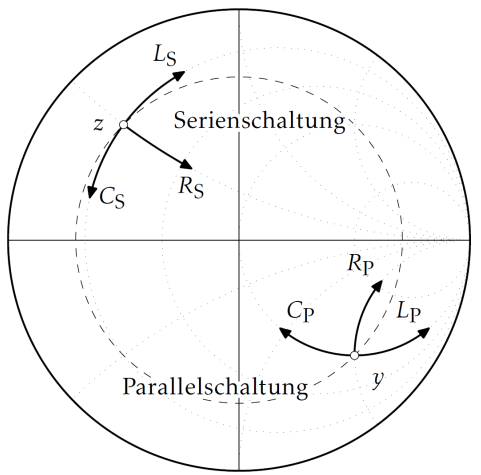
\includegraphics[width=.45\columnwidth]{Figures/Smithdiagramm_Zusammenschaltungen.png}
% \end{center}

%\columnbreak

\subsection{Maxima und Minima bei stehender Welle}
Bei \textbf{verlustloser} Leitung:
\begin{align*}
	&U_{\texttt{max}} = |U_h| \cdot (1+|r(l)|) & U_{\texttt{min}} = |U_h| \cdot (1-|r(l)|) &\\
	&I_{\texttt{max}} = \left | \frac{U_h}{Z_L} \right | \cdot (1+|r(l)|) & I_{\texttt{min}} = \left| \frac{U_h}{Z_L} \right | \cdot (1-|r(l)|) &
\end{align*}
Für \textbf{Spannungen}: Abstand von der Last $ z $ 
\begin{align*}
	 &z_{\texttt{min}} = \frac{\lambda}{4\pi}(\theta_{rad}+(2n+1)\pi)&
	 z_{\texttt{max}} = \frac{\lambda}{4\pi} \cdot (\theta_{rad}+2n\pi)&\\
	 \Aboxed{&\text{\textbf{Minima} alle}\: \frac{\lambda}{2} \rightarrow \frac{l}{\lambda}=0.5} \Aboxed{&
	 	\text{\textbf{Maxima} alle}\: \frac{\lambda}{4} \rightarrow \frac{l}{\lambda}=0.25} &
\end{align*}
$ \rightarrow $ Schnittpunkte mit der reellen Achse!
\subsection[Von Last zu Quelle]{Lastseite $\rightarrow$ Quelle}
\begin{enumerate}
    \item $Z_L = Z_B$ ins Diagramm einzeichnen
    \item Lastimpedanz bestimmen,
          wenn z.B. Parallelschaltung etc.
    \item Normieren
          \[\underline{z}_n = \frac{\underline{Z}(l)}{Z_L} \]
    \item Im Chart eintragen
    \item Linie vom Mittelpunkt durch $\underline{z}_ns$ nach außen

          Ablesen und Notieren:

          $\rightarrow$ Relative Länge $\left[\frac{l}{\lambda}\right]$

          $\rightarrow$ Relativer Winkel in \textbf{Degree}
    \item Kreis einzeichen

          Ablesen und Notieren:

          $\rightarrow$ \textbf{Maxima}: rechter Schnittpunkt mit Re-Achse

          $\rightarrow$ \textbf{Minima}: linker Schnittpunkt mit Re-Achse

          $\rightarrow$ $ \underline{r} $ abmessen und aus oberer Skala auslesen
    \item Um Leitungslänge im UZS laufen
          $\rightarrow$ Linie vom Mittelpunkt durch neuen Punkt nach außen

          Ablesen und Notieren:

          $\rightarrow$Relativer Winkel
    \item Wenn $\alpha\neq 0$

          $\rightarrow$ Dämpung ausrechen
          $\rightarrow$ Um Faktor nach innen Spiralieren

    \item Dieser Punkt ist $\underline{z}_e$
    \item Eingangsimpedanz ablesen
          \[\underline{Z}_E = \underline{z}_e \cdot Z_L\]
\end{enumerate}


\usetikzlibrary{decorations.pathmorphing}
\usetikzlibrary{decorations.text}
\tikzset{
cross/.style={cross out, draw=black, minimum size=2*(#1-\pgflinewidth), inner sep=0pt, outer sep=0pt},
%     %default radius will be 1pt. 
cross/.default={3.5pt}
dot/.style={circle, fill=#1, inner sep=0, minimum size=4pt},
mini dot/.style={circle, inner sep=0pt, minimum size=2pt, pos=1, fill, node contents={}},
}
\begin{center}
 \begin{tikzpicture}    
    
    %Außenkreis
    \draw[-](0,0) circle (2);

    %Realteil Linien
    \draw[-, black!50](-2,0)--(2,0);

    \draw[dotted, black!50](0.4,0) circle (1.6);
    \draw[dotted, black!50](0.8,0) circle (1.2);
    \draw[dotted, black!50](1.2,0) circle (0.8);
    \draw[dotted, black!50](1.6,0) circle (0.4); 

    
    %Imaginärteil Linien
    \draw[-, black!50](0,-2)--(0,2);

    \draw[dotted, black!50, xshift = 13.25ex, yshift = -31.98ex](135:4.84)arc(135:90:4.84);
    \draw[dotted, black!50, xshift = 13.25ex, yshift = -13.25ex](180:2)   arc(180:90:2);
    \draw[dotted, black!50, xshift = 13.25ex, yshift = -5.485ex](225:.828)arc(225:90:.828);

    \draw[dotted, black!50, xshift = 13.25ex, yshift = 31.98ex](270:4.84)arc(270:225:4.84);
    \draw[dotted, black!50, xshift = 13.25ex, yshift = 13.25ex](270:2)   arc(270:180:2);
    \draw[dotted, black!50, xshift = 13.25ex, yshift = 5.485ex](270:.828)arc(270:135:.828);

    %Reflexionsfaktorkreis
    \draw[dashed](0,0) circle (1.3);

    %Serienschaltung
    \draw[-,fill=black!100] (-.919,.919) circle (0.025)node[left, yshift =.5] {\tiny z}node[right]{\tiny Serienschaltung};
    \draw[latex-latex, xshift = 2.65ex](125:1.6)node[above, yshift=-.75ex]{\scriptsize${L_s}$} arc (125:165:1.6)node[below, yshift=.5ex]{\scriptsize$C_s$};
    \draw[latex-, xshift = 13.25ex, yshift = 33.75ex](241:5.1)node[below, yshift=.5ex]{\scriptsize$R_s$}arc(241:235:5.1);

    %Parallelschaltung
    \draw[-,fill=black!100] (.919,-.919) circle (0.025)node[above left, xshift = .5ex]{\tiny y} node[below]{\tiny Parallelschaltung};
    \draw[-latex, xshift = 13.25ex, yshift = -7.25ex](170:1.1)arc(170:140:1.1)node[above, yshift=-.75ex]{\scriptsize$R_p$};

    \draw[latex-latex, xshift = 7.12ex](293:.925)node[right, xshift = -.95ex]{\scriptsize$L_p$}arc(293:227.5:.925)node[left, xshift = .85ex]{\scriptsize$C_p$};

\end{tikzpicture}
\end{center}

Positive/negative Blindwerte bewegen sich im/gegen den Uhrzeigersinn. Wirkwiderstände bewegen sich immer zum Leerlaufpunkt.

\subsection{Vorgehen mit geg. Eingangswiderstand}
Wenn mit dem Smith-Diagramm gearbeitet
wird, liefert dies die Schritte \ref{Ref L_anfang} und \ref{Bestimmen Z_E}
\begin{enumerate}
	\item Lastimpedanz
	\[ \underline{Z}_A = \dfrac{1}{\frac{1}{R_A} + j \omega C_A} \]
	\item Reflexion am Leitungsende
	\[ \underline{r}_A = \underline{r}(z=0) = \dfrac{Z_A - \underline{Z}_L}{Z_A + \underline{Z}_L} \]
	\item Reflexion am Leitungsanfang \label{Ref L_anfang}
	\[ \underline{r}_E = \underline{r}(z=d) =  \underline{r}_A \cdot e^{-j 2 \beta d}\]
	\item Bestimmung der Impedanz \label{Bestimmen Z_E}
	\[ \underline{Z}_E = \underline{Z}_L \cdot \dfrac{1 + \underline{r}_E}{1 - \underline{r}_E}\]
	\item Eingangswiderstand
	\[ \underline{Z}_E = \dfrac{1}{\frac{1}{\underline{Z}_E} + j \omega C_E}\]
\end{enumerate}

\subsection{Reihen- und Parallelschaltung}
Leitung transformiert den Abschluss
\[ \underline{Z}_2 = R_2 + jX_2 \quad \text{bzw.} \quad \underline{Y}=G_2 + jB_2\]
mit \[ \underline{Y}_2=\frac{1}{Z_2}  \]

\subsubsection{ESB Serienschaltung}
\[ P = \frac{\hat{I}^2_2 \cdot R_2}{2} \Rightarrow \hat{I}(l) = I^2_2 \cdot \sqrt{\frac{R_2}{R(l)}} \]
    \section{Antennen}
\subsection{Herz'scher Dipol (HDp)}
\boxed{\vec{p} = Q\cdot\vec{d}}
\subsubsection{Allgemein}

{\footnotesize\begin{empheq}[box=\fbox]{align*}
        {\vec{H}} & =-\frac{I_0\Delta l'\beta^2}{4\pi}e^{-j\beta R}\cdot\sin\theta\left(\frac{1}{j\beta R}+\frac{1}{(j\beta R)^2}\right)\vec{e}_\phi                                 \\
        {\vec{E}} & = -\frac{Z_F I_0\Delta l'\beta^2}{2\pi}e^{-j\beta R}\cdot\cos\theta\left(\frac{1}{(j\beta R)^2}+\frac{1}{(j\beta R)^3}\right)\vec{e}_R                           \\
        & = -\frac{Z_F I_0\Delta l'\beta^2}{4\pi}e^{-j\beta R}\cdot\sin\theta\left(\frac{1}{(j\beta R)}+\frac{1}{(j\beta R)^2}+\frac{1}{(j\beta R)^3}\right)\vec{e}_\theta
    \end{empheq}}%

\subsubsection[Nahfeld]{Nahfeld (Fresnel-Zone):\\ $\frac{\lambda}{2\pi R}\gg 1$ oder $\beta R \ll 1$}

Überwiegend \textbf{Blindleistungsfeld}, da $E$ zu $H$ $90^\circ$
phasenverschoben
\begin{empheq}[box=\fbox]{align*}
    \vec{H} & \approx \frac{I_0 \Delta l'}{4\pi R^2}\cdot\sin\theta\cdot\vec{e}_\phi                                            \\
    \vec{E} & \approx \frac{I_0 \Delta l'}{2\pi j \omega\varepsilon R^3}\cos\theta\cdot\vec{e}_R\\
    & +       \frac{I_0 \Delta l'}{4\pi j \omega\varepsilon R^3}\sin\theta\cdot\vec{e}_\theta
\end{empheq}

\subsubsection[Fernfeld]{Fernfeld (Fraunhofer-Zone):\\ $\frac{\lambda}{2\pi R}\ll 1$ oder $\beta R\gg 1$}

Überwiegend \textbf{Wirkleistungsfeld}, $\vec{S}$ nach außen somit Kugelwelle

\vspace{1ex}
mit $\eta = Z_{F0}$

\begin{empheq}[box=\fbox] {align*}
    H & \approx  j\frac{\beta I_0 \Delta l'}{4\pi R}\cdot e^{-j\beta R}\cdot\sin\theta\cdot\vec{e}_\phi                           \\
    E & \approx  j\frac{\beta Z_F I_0 \Delta l'}{4\pi R}\cdot e^{-j\beta R}\cdot\sin\theta\cdot \vec{e}_\theta
\end{empheq}

\subsubsection{Abgestrahlte Leistung im Fernfeld HDp}
\begin{align*}
    P_\texttt{rad} = P_s & = \frac{Z_{F0} {I_0}^2 \beta^2 (\Delta l')^2}{12\pi}                             \\
                   & = \frac{I_0^2 Z_F\pi}{3}\cdot \dfrac{\Delta l'^2}{\lambda^2}                     \\
                   & = 40\pi^2\Omega\cdot\left(\frac{I_0\Delta l'}{\lambda}\right)^2                  \\
    S_{av}         & = \frac{Z_FI_0^2\beta^2(\Delta l')^2}{32\pi^2R^2}\cdot\sin^2\theta\cdot\vec{e}_R \\
                   & = \frac{1}{2}\Re\left\{\vec{E}\times\vec{H}^*\right\}
\end{align*}
\subsubsection{Strahlungswiderstand HDp}
\begin{align*}
    R_s & = \frac{2}{3}\pi Z_F\left(\frac{\Delta l'}{\lambda}\right)^2
    = 80\pi^2\Omega\left(\frac{\Delta l'}{\lambda}\right)^2
\end{align*}
\subsubsection{Verlustwiderstand HDp}
\begin{align*}
    R_{v} & = \frac{l}{\sigma\cdot A_\delta}
\end{align*}
\subsection{Magnetischer Dipol}
\boxed{\vec{m} = \vec{I}\pi\vec{a}^2\vec{e}_z}
\boxed{m = I\cdot A}
\begin{center}
    \usetikzlibrary{shapes.geometric}

\tikzset{elliparc/.style args={#1:#2:#3}{%
insert path={(#1:#3) arc (#1:#2:#3)}}}
\begin{tikzpicture}

    %Elipse
    \node[ellipse,
        draw = black,
        dashed,
        minimum width = 3cm,
        minimum height = 1cm] (e) at (0,0) {};
    
    %Punkte
    \fill[](0,0)        circle(.05);
    \fill[](1.75,2.5)   circle(.05)
        node[right]{\tiny{P(R,$\theta$,$\phi$)}};
    \fill[](1.25,0.255) circle(.05)
        node[above right]{\tiny{P'}};
    \fill[](1.75,0.375) circle(.05)
        node[above right]{\tiny{P''}};

    %Koordinaten Achsen
    \draw[-latex](0,0)--(-1.5,-1) node[right]{x};
    \draw[-latex](0,0)--(1.5,-1) node[left]{y};
    \draw[-latex](0,0)--(0,3) node[left]{z};
    
    %Pfeile
    \draw[-latex, blue](0,0)--(1.75,2.5)
        node[above, midway, left]{\tiny{$\vec{R}$}};
    \draw[-latex, blue](1.25,0.255)--(1.75,2.5)
        node[midway, below left]{\tiny{$\vec{R}_1$}};
    \draw[-latex, blue](0,0) -- (1.25,0.255)
        node[above, midway]{\tiny{\tiny{R}'}};
    \draw[-latex, red](-0.9,0.4)--(-.95,.385)
        node[above]{I};
    \draw[-latex](1.25,0.255)--(1,0.4)
        node[above]{\tiny{dl'}};
    \draw[-latex](1.75,2.5)--(1.5,2.65)
        node[above]{\tiny$\vec{A}$};
    \draw[-latex](0,0)--(-1.5,-0)
        node[above, midway]{\tiny$\vec{a}$};
   
    %Winkel
    \draw[-] (90:1) arc (90:55:1)
    node[above, midway] {\tiny{$\theta$}};
    \draw[] (0,0) [elliparc=-117:30:.75cm and .25cm];
    \node[yshift=-4.5]{\tiny{$\phi$'}};
    
    %Legende
    \node[right] at (-0.75,-0.75){\tiny{$\vec{m}=\vec{I}\pi a^2\vec{e}_z$}};
   
    %Linien
    \draw[dashed](0,0)--(2.5,0.5);
    \draw[dashed](1.75,0.375)--(1.75,2.5);

\end{tikzpicture}

\end{center}

\begin{align*}
    \vec{A}  & = \frac{\mu m}{4\pi R^2}(1+j\beta R) e^{-j\beta R}\sin\theta\cdot\vec{e}_\phi \\
    \Delta l & \rightarrow \beta\pi\ a^2
\end{align*}

{\footnotesize\begin{empheq}[box=\fbox]{align*}
    {\vec{H}}   & = -\frac{j\omega\mu\beta^2m}{2\pi Z_{F0}}e^{-j\beta R}\cdot\cos\theta\left(\frac{1}{(j\beta R)^2}+\frac{1}{(j\beta R)^3}\right)\vec{e}_R                             \\
    & = -\frac{j\omega\mu\beta^2m}{4\pi Z_{F0}}e^{-j\beta R}\cdot\sin\theta\left(\frac{1}{(j\beta R)}+\frac{1}{(j\beta R)^2}+\frac{1}{(j\beta R)^3}\right)\vec{e}_\theta   \\
    {\vec{E}}   & =  \frac{j\omega\mu\beta^2m}{4\pi}e^{-j\beta R}\sin\theta\left(\frac{1}{j\beta R}+\frac{1}{(j\beta R)^2}\right)\vec{e}_\phi
\end{empheq}}%

\subsubsection{Fernfeld}
\begin{empheq}[box=\fbox]{align*}
    E & \approx -\frac{\beta m\omega\mu}{4\pi R}e^{-j\beta R}\sin\theta\cdot\vec{e}_\phi \\
    H & \approx -\frac{\beta m\omega\mu}{4\pi R Z_{F0}}e^{-j\beta R}\sin\theta\cdot\vec{e}_\theta
\end{empheq}
\subsubsection{Abgestrahlte Leistung im Fernfeld}
\begin{align*}
    P_\texttt{rad} & = \frac{Z_F\beta^4m^2}{12\pi}                                     \\
                   & = \frac{m^2\mu\omega^4}{12\pi v_p^3}                              \\
    S_{av}         & = \frac{Z_F\beta^4m^2}{32\pi^2R^2}\cdot\sin^2\theta\cdot\vec{e}_R \\
                   & = \frac{1}{2}\Re\left\{\vec{E}\times\vec{H}^*\right\}
\end{align*}

\subsubsection{Nahfeld}
\begin{empheq}[box=\fbox]{align*}
    E & \approx -\frac{jm\omega\mu}{4\pi R^2}\sin\vartheta\cdot\vec{e}\varphi \\
    H & \approx \frac{m}{4\pi R^3}(2\cos\theta\cdot\vec{e}_R+\sin\vartheta\cdot\vec{e}_\vartheta)
\end{empheq}
\newpage
\subsection{Lineare Antenne}
Stromverteilung auf linearen Antennen \textbf{nicht} konstant:
\begin{align*}
    I(z') & = I_0\cdot\sin\left[\beta\left(\frac{L}{2}-|z'|\right)\right]
\end{align*}

\subsubsection{Dipolantenne allgemein}
\begin{align*}
    \vec{\underline{H}}      & = j\frac{I_0}{2\pi R}\cdot e^{-j\beta r}\cdot\frac{\cos\left[\left(\frac{\beta L}{2}\right)\cos\theta\right]-\cos\left(\frac{\beta L}{2}\right)}{\sin\theta}\cdot\vec{e}_\varphi         \\
    \vec{\underline{E}}      & = H\cdot Z_{F0}\cdot\vec{e}_\vartheta                          \\
    I_0          & = \sqrt{\frac{2\cdot P_{s}}{R_{s}}} \qquad R_{s} \rightarrow \text{siehe Tabelle!}                                
\end{align*}
\textbf{Halbwellen}dipol: $ l=\frac{\lambda}{2} \qquad \underline{Z}_{s}=(73,13+j42,54)\Omega$\\

\textbf{Ganzwellen}dipol: $ l=\lambda \qquad \underline{Z}_{s}=(199,09+j125,41)\Omega$

\subsubsection{Eingangs-/Fußpunktimpedanz}
\begin{align*}
	\underline{Z}_A=\underline{Z}_s\frac{|I_0|^2}{|I_0(z'=0)|^2} = \frac{\underline{Z}_s}{\sin^2\left[ \beta \frac{l}{2} \right] }
\end{align*}

Strom am Fußpunkt:
\begin{align*}
	I(z'=0) & = I_0\cdot\sin\left[\beta\left(\frac{L}{2}\right)\right]
\end{align*}
komplexe Strahlungsleistung:
\begin{align*}
	P_s +jQ_s = \underline{Z}_s\cdot \frac{|I_0|^2}{2} = \underline{Z}_A \cdot \frac{|I_0(z'=0)|^2}{2}
\end{align*}

\subsubsection{Strahlleistungsdichte}
\begin{align*}
    \vec{S}_{av} & = \frac{Z_FI_0^2}{8\pi^2 R^2}\left(\frac{\cos\left(\frac{\beta L}{2}\cos\vartheta\right)-\cos\left(\frac{\beta L}{2}\right)}{\sin\vartheta}\right)^2\cdot\vec{e}_R                               \\
    S_{av} & = S_{max} \cdot D(\vartheta, \varphi) = S_{max} \cdot C^2(\vartheta, \varphi)
\end{align*}
\subsubsection{Strahlungsleistung}
\begin{align*}
    P_{rad}          & = \frac{Z_{F0}I_0^2}{4\pi}\int^{\theta=\pi}_{\theta=0}\frac{\left(\cos\left(\frac{\beta L}{2}\cos\theta\right)-\cos\left(\frac{\beta L}{2}\right)\right)^2}{\sin\theta}\cdot\vec{e}_\theta \\
                 & = \int_A S_{AV}\cdot d\vec{a}                                                                                                                                                              \\
                 & = \int^{2\pi}_{\Phi = 0}\int^{\pi}_{\Theta = 0} S_{AV} R^2 \sin\Theta \cdot d\Theta \cdot d\Phi
\end{align*}

\subsection{Antennenkenngrößen}

\makebox[0pt][l]{
    \begin{minipage}[b]{0.25\columnwidth}
        \resizebox{1.85\columnwidth}{!}{
            \begin{circuitikz}
                \draw(0,3.5) node[below]{$l$}
                to[R=$R_V$](3,3.5)
                to[R=$R_S$](3,1.5)
                to[L=$jX_A$](3,0)
                to[short](0,0) node[above]{$l'$}
                to[open, o-o](0,3.5);
                \draw[latex-, double](1.5,1.75)--(0.5,1.75) node[left]{$\underline{Z}_A$};
            \end{circuitikz}
        }
    \end{minipage}
    \begin{minipage}[b]{0.25\columnwidth}
        \begin{tikzpicture}
            \node[]{};
        \end{tikzpicture}
    \end{minipage}

    \begin{minipage}[b]{0.5\columnwidth}
        \footnotesize
        \begin{align*}
            \underline{Z}_A & := \text{Antennenimpedanz}        \\
            R_V             & := \text{Verlustwiderstand}       \\
            R_S             & := \text{Strahlungswiderstand}    \\
            X_A             & := \text{Antennenblindwiderstand} \\
            D               & := \text{Directifity/Richtfaktor} \\
            G               & := \text{Gain/Gewinn}             \\
            A_{eff}         & := \text{Wirksame Antennenfläche} \\
        \end{align*}
        \normalsize
    \end{minipage}
}

\subsubsection{Abgestrahlte Leistung}
\begin{align*}
    P_s = P_{rad} & = \frac{1}{2}\cdot I_A^2 \cdot R_S
\end{align*}
\subsubsection{Verlustleistung}
\begin{align*}
    P_V & = \frac{1}{2}\cdot I_A^2\cdot R_V
\end{align*}
\subsubsection{Wirkungsgrad}
\begin{align*}
    \eta & = \frac{P_S}{P_S + P_V} = \frac{R_S}{R_S + R_V}
\end{align*}

\subsubsection{Richtcharakteristik}
$C_{i} \ent$ isotroper Kugelstrahler als Bezugsgröße in Hauptabstrahlrichtung
\begin{align*}
 	C_{i}(\vartheta, \varphi) & = \frac{E(\vartheta, \varphi)}{E_{i}}=\frac{H(\vartheta, \varphi)}{H_{i}}                                               & C_{i}>1\\
    C(\vartheta, \varphi)     & = \frac{E(\vartheta, \varphi)}{E_{\max}}=\frac{H(\vartheta, \varphi)}{H_{\max}} = \frac{U(\vartheta,\varphi)}{U_{\max}} & 0 \leq C(\vartheta, \varphi) \leq 1 \\
    C(\vartheta, \varphi) &= 
    \left|\frac{\cos\left(\frac{\beta L}{2}\cos\vartheta\right)-\cos\left(\frac{\beta L}{2}\right)}{\sin\vartheta}\right|
\end{align*}

\subsubsection{Richtfunktion/-faktor}
%In $[\si{dB}]$ angeben!
\begin{align*}
    D(\vartheta, \varphi) & = \frac{S(\vartheta, \varphi)}{S_{i}} = C^\mathbf{2}_i(\vartheta, \varphi) = D \cdot C^{2}(\vartheta, \varphi) &\\
    D & = \max \{D(\vartheta, \varphi)\} = \frac{S_{\max}}{S_{i}}&
\end{align*}
\begin{align*}
	&\text{Halbwellendipol} &D(\vartheta, \varphi) &= 
	\left(\frac{\cos\left(\frac{\pi}{2}\cos\vartheta\right)}{\sin\vartheta}\right)^\mathbf{2}& = C^2(\vartheta, \varphi)\\
	&\text{Ganzwellendipol} &D(\vartheta, \varphi) &= 
	\left(\frac{\cos\left(\pi\cos\vartheta\right)+1}{\sin\vartheta}\right)^\mathbf{2}& =C^2(\vartheta, \varphi)
\end{align*}

\subsubsection{Gewinn/Gain}
Verlustlose Antenne, wenn $ \eta = 1 $
\begin{align*}
    G & = \eta \cdot D \qquad \text{bei}\;  \eta=1 \rightarrow  G=D
%    \qquad [\si{dB}]
\end{align*}

\subsubsection{Wirksame Antennenfläche}
\begin{align*}
	P_e &= \frac{1}{2}\cdot R_L \cdot I^2 = \frac{U_0^2}{8P_{rad}} & S_s &= \frac{1}{2} \, E \, H = \frac{1}{2}\, H^2 \, Z_{F0} = \frac{1}{2} \, \frac{E_0^2}{Z_{F0}}  \\
	A_\texttt{eff} & = \frac{P_e}{S_s} = \frac{U_0^2}{8P_{rad}}\frac{2Z_F}{E_0^2} &
    A_\texttt{eff} & = \frac{\lambda^2}{4\pi}\cdot G = \dfrac{Z_{F0}}{4 R_S} \cdot l_\texttt{eff}^2&
\end{align*}
Beim Hertzschen Dipol:
\begin{align*}
	A_\texttt{eff} & = \frac{\lambda^2}{4\pi}\cdot\frac{3}{2}\sin\theta &
	A_\texttt{eff} & = \frac{\lambda^2}{4\pi}\cdot G = \dfrac{Z_{F0}}{4 R_S} \cdot l_\texttt{eff}^2 &
\end{align*}

\subsection{Bezugsantennen}
\[
    \boxed{g = 10 \cdot log(G) \si{dB}}
\]

mit $P_0$ : Eingangsleistung der Antenne

\begin{description}
    \item \textbf{\underline{G$\rightarrow$Bezugsantenne:}}

          Elementardipol  zu Kugelstrahler \[D = 1,50 \rightarrow g = 1,76\si{dBi}\]
          Halbwellendipol zu Kugelstrahler \[D = 1,64 \rightarrow g = 2,15\si{dBi}\]

    \item \textbf{\underline{EIRP}: Eqivalent \underline{Isoropic} Radiated Power}
          \[
              \text{EIRP} = P_0 \cdot G_i [\si{dBi}]
          \]

    \item \textbf{\underline{ERP}: Eqivalent Radiated Power (verlustloser Halbwellendipol)}
          \[
              \text{ERP} = P_0 \cdot G_d [\si{dBd}]
          \]
\end{description}

\subsection{Senden und Empfangen}
\begin{center}
    \resizebox{0.75\columnwidth}{!}{
        \begin{circuitikz}
            %Schaltbild
            \draw(0,0) node[below right]{$U_0=l_{\texttt{eff}}\cdot E_0$}
            to[V,v=$U_0 $](0,2)                               %Spannungsquelle
            to[R=$R_{s}$](2,2)                                   %Strahlungswiderstand
            to[short](4 ,2)
            to[R= $R_{s}$](4,0)
            to[short](0,0);
            \draw(3,2) node[below]{$1$}
            to[open,o-o](3,0) node[above]{$1'$};

        \end{circuitikz}
    }
\end{center}


\begin{description}
    \item Senden = transmit = TX
    \item Empfangen = receive = RX
\end{description}

\begin{align*}
    \frac{P_{RX}}{P_{TX}}          & = A_{\texttt{eff},RX}\cdot A_{\texttt{eff},TX}\cdot\frac{1}{\lambda^2r^2}                          \\
                                   & = D_{i,RX}\cdot\eta_{RX}\cdot D_{i,TX}\cdot\eta_{TX}\cdot\left(\frac{\lambda}{4\pi r}\right)^2     \\
    \Aboxed{A_\texttt{eff}(\theta) & = G_{RX}\cdot\frac{\lambda^2}{4\pi}\overbrace{\cdot\frac{3}{2}\cdot\sin^2\theta}^{{D_{i,\theta}}}} \\
    P_{RX}                         & = S_{RX}\cdot A_\texttt{eff}                                                                       \\
                                   & = P_{TX}\cdot G_{TX}\cdot G_{RX}\cdot \left(\frac{\lambda}{4\pi r}\right)^2
\end{align*}

\subsubsection{Freiraumdämpfung/Freiraumdämpfungsmaß}
\begin{align*}
    F = \dfrac{P_{TX}}{P_{RX}} \cdot \left(\dfrac{4 \pi d}{\lambda}\right)^2                         & \qquad [1]       \\
    a_{0} = 20 \lg \left(\frac{4 \pi d}{\lambda}\right) =20 \lg \left(\frac{4 \pi d f}{c_{0}}\right) & \qquad [\si{dB}]
\end{align*}

\subsubsection{Leistungspegel/Freiraumpegel}
\begin{align*}
    L      & = 10 \lg \left(\frac{P}{1 \si{mW}}\right) \qquad [\si{dBm}] \\
    L_{RX} & = L_{TX}+g_{TX}+g_{RX}-a_{0} \qquad [\si{dB}]
\end{align*}

\end{multicols*}
\subsection{Richtcharakteristik Dipolantennen}
%\begin{minipage}{\linewidth}
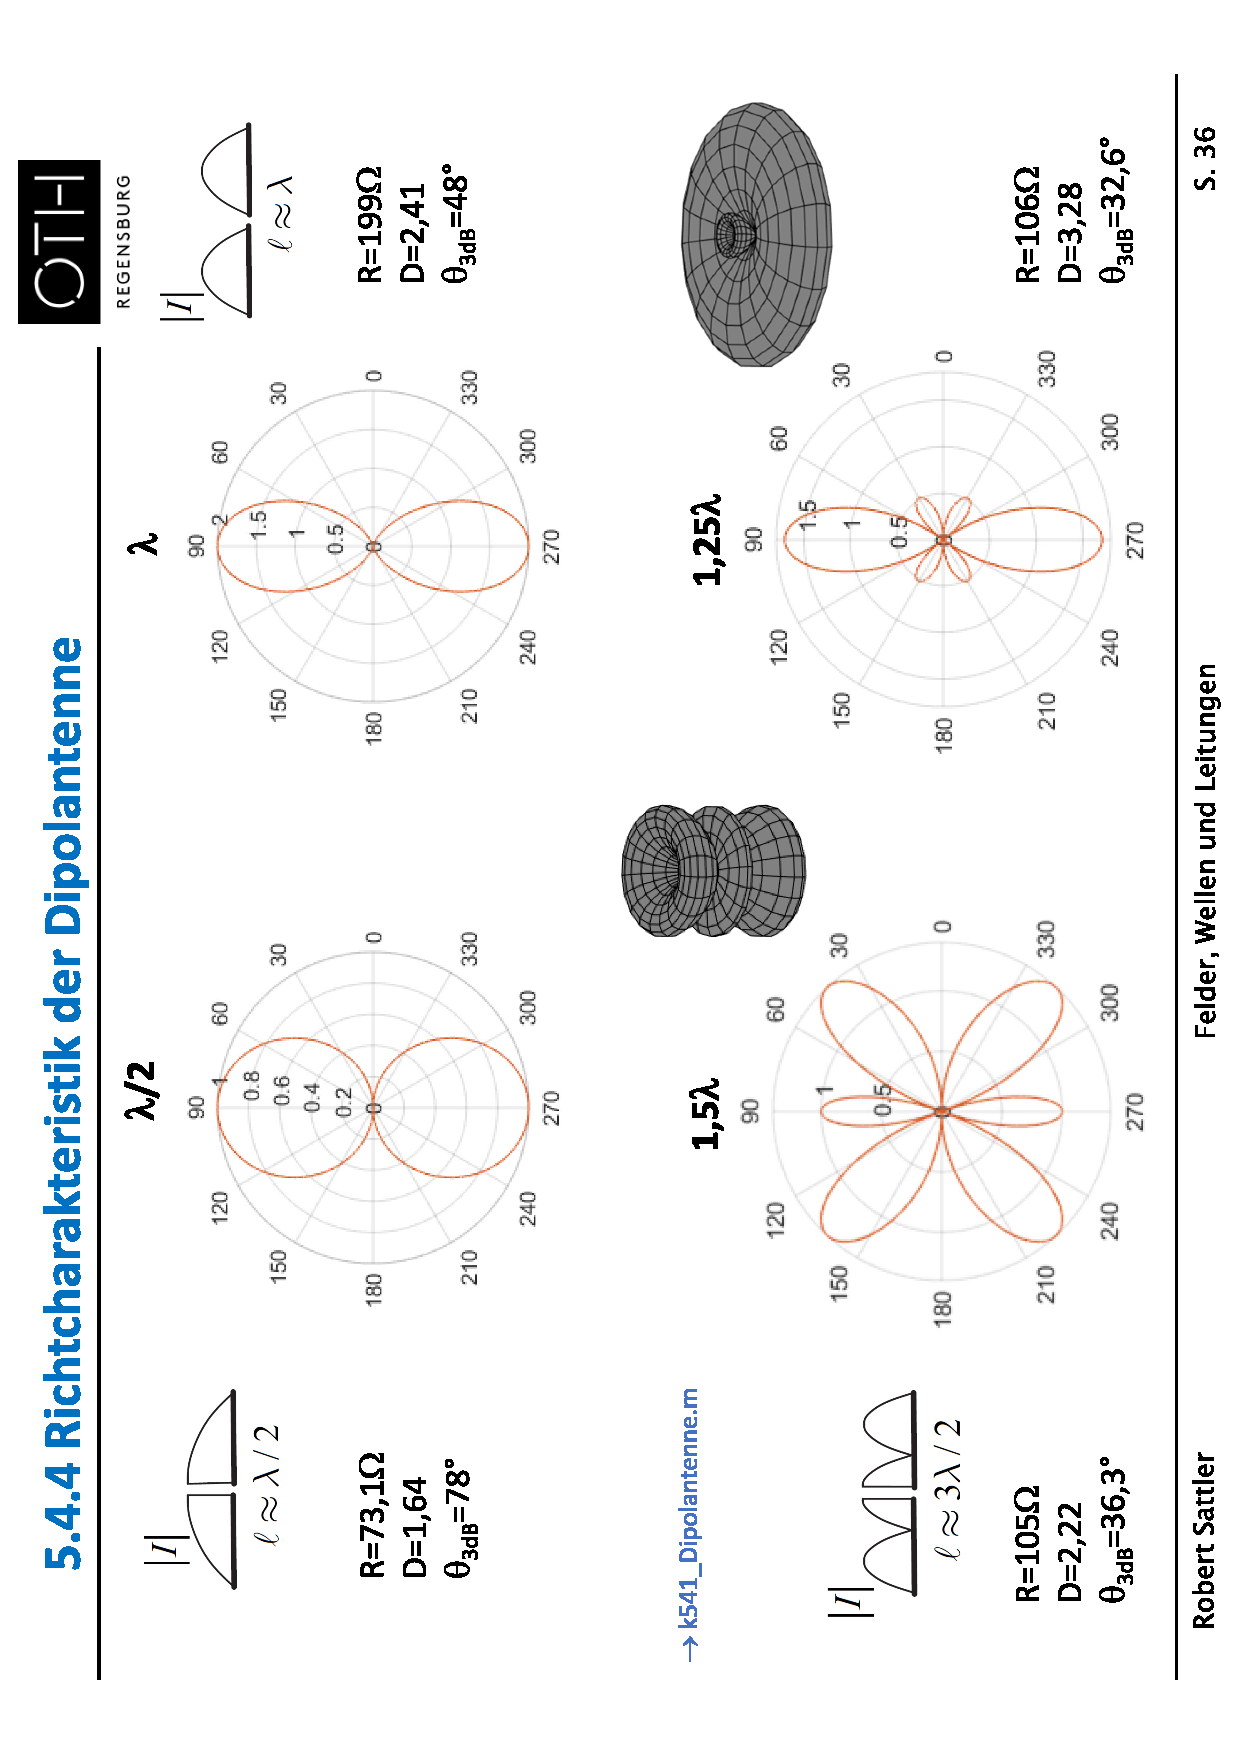
\includegraphics[angle=-90, width=0.93\linewidth]{Figures/Dipolantenne_Richtcharakteristik.pdf}
%\end{minipage}
\subsection{Blindwiderstand Dipolantennen}
%\begin{minipage}{\linewidth}
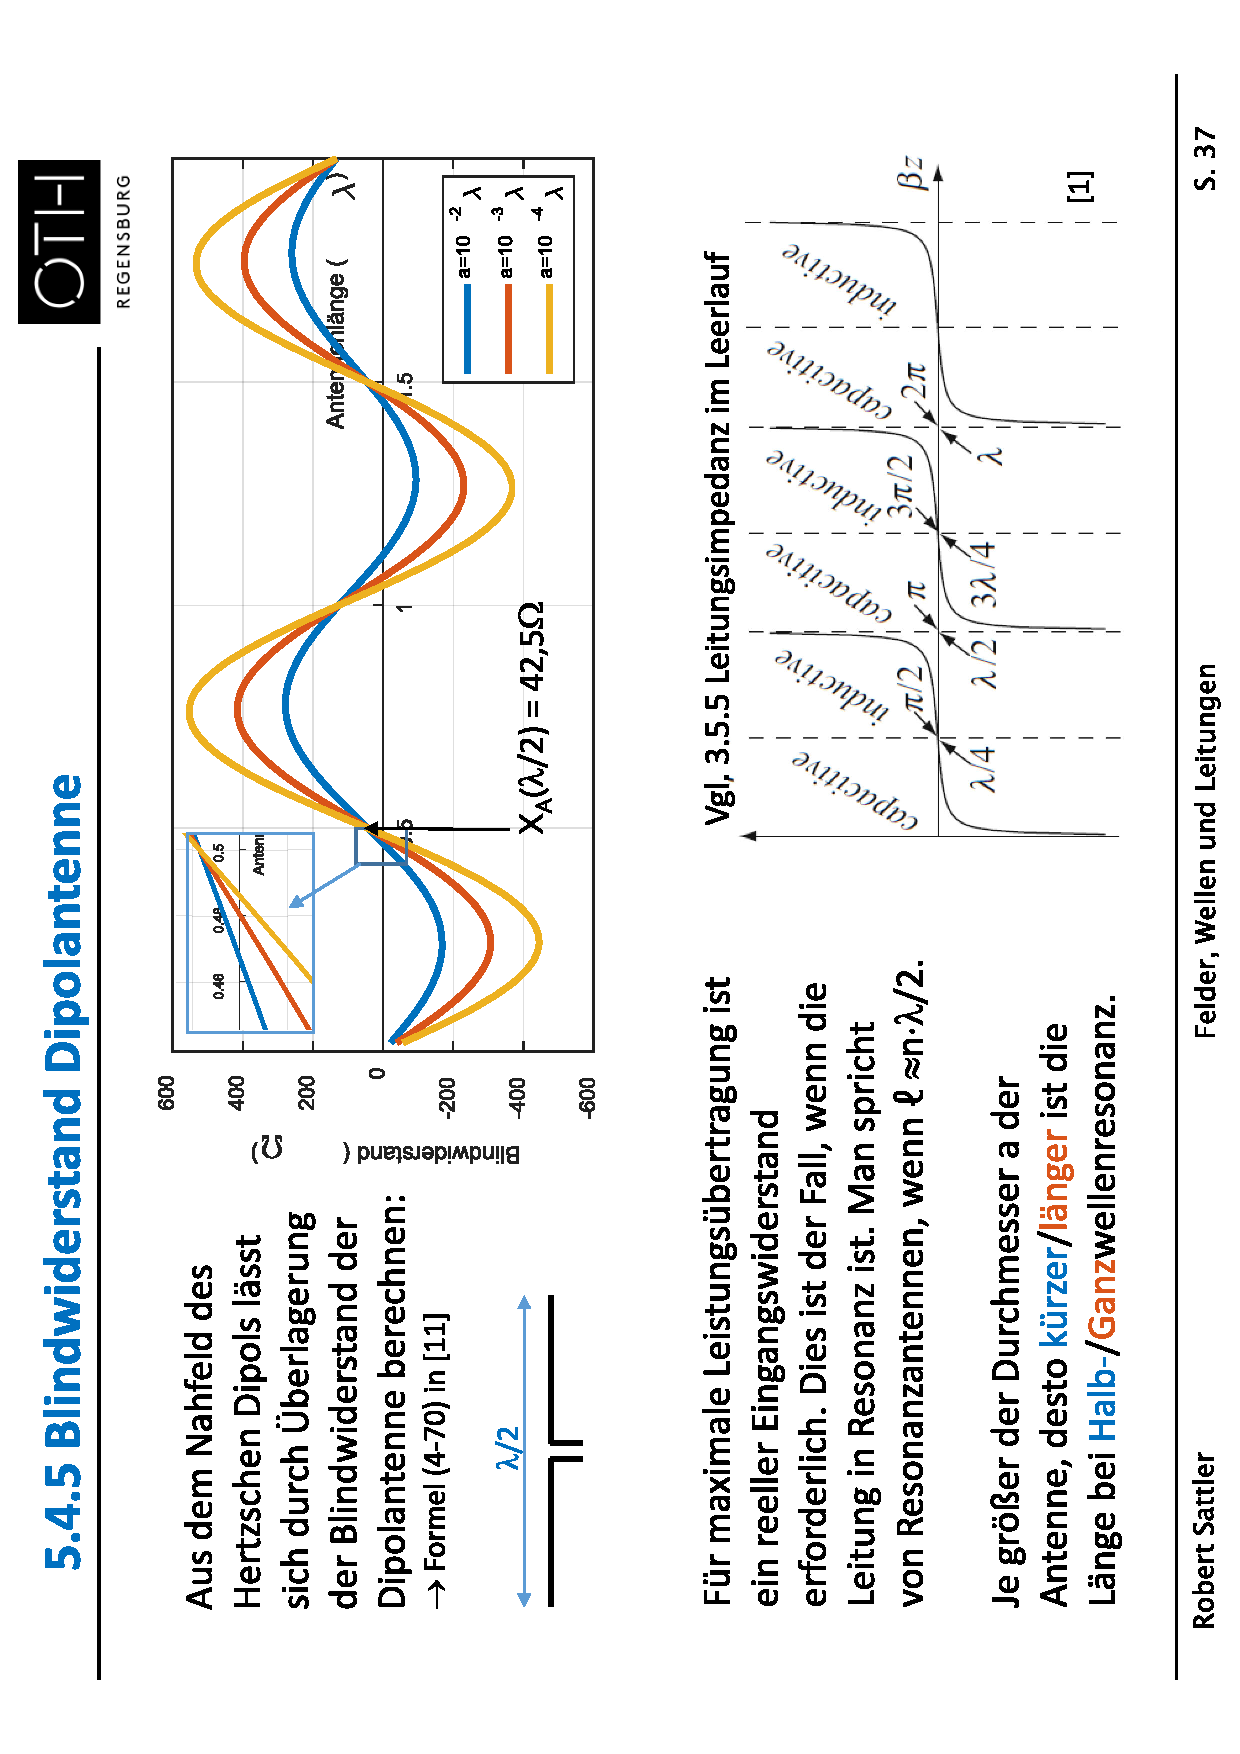
\includegraphics[angle=-90, width=0.93\linewidth]{Figures/Dipolantenne_Blindwiderstand.pdf}
%\end{minipage}
\newpage
\subsection{Antennentabelle}\label{sec:Antennentabelle}
\begin{minipage}{1.7\columnwidth}
    \includegraphics[width=.55\columnwidth]{Figures/Antennentabelle_1.png}\\
    \includegraphics[width=.55\columnwidth]{Figures/Antennentabelle_2.png}
\end{minipage}
\section{Einheiten}
% \begin{table}
\begin{NiceTabular}{c|l|l}[cell-space-limits=3pt]
    \hline
    Symbol & Größe & Einheit\\
    \hline 
    A, W & Arbeit, Energie & J = VAs = Ws\\
    $\vec{A}$ & mag. Vektorpotenzial & $\dfrac{Vs}{m} = \dfrac{Wb}{m}$ ($\vec{B}$ = $\nabla \times \vec{A}$)\\
    $\vec{B}$ & mag. Flussdichte & $T = \dfrac{Vs}{m^2}$\\
    C & Kapazität & $F = \dfrac{As}{V}$\\
    $\vec{D}$ & dielek. Verschiebung/Erregung & $\dfrac{As}{m^2}$\\
    e, q, Q & (Elementar-)ladung & C = As\\
    $\vec{E}$ & elek. Feldstärke & $\dfrac{V}{m}$ \\
    $\vec{H}$ & mag. Feldstärke/Erregung & $\dfrac{A}{m}$\\
    $\vec{J}$ & Stromdichte & $\dfrac{A}{m^2}$\\
    $\vec{J}_F$ & Flächenstromdichte & $\dfrac{A}{m}$\\
    $\vec{M}$ & Drehmoment & J = Nm = VAs\\
    F & Kraft & $\dfrac{kgm}{s} = N$\\
    $R_{mag}$ & mag. Widerstand & $\dfrac{S}{s} = \dfrac{A}{Vs}$\\
    $\vec{S}$ & Poynting-Vektor & $\dfrac{W}{m^2}$\\
    Z & Wellenwiderstand & $\Omega$\\
    $\delta_s$ & Eindringtiefe & m \\
    $\varepsilon$ & Dielektrizitätskonstante & $\dfrac{As}{Vm}$\\
    $\varphi$ & elek. Skalarpotenzial & V \\
    $\varphi_m$ & mag. Skalarpotenzial & A \\
    $\rho$ & Raumladungsdichte & $\dfrac{As}{m^3}$\\
    $\rho$ & spez. Widerstand & $\dfrac{\Omega}{m} = \dfrac{VA}{m}$\\
    $\kappa, \sigma$ & elek. Leitfähigkeit & $\dfrac{S}{m} = \dfrac{A}{Vm}$\\
    $\lambda$ & Wellenlänge & m\\
    $\mu$ & Permiabilitätskonstante & $\dfrac{Vs}{Am}$\\
    $\Phi_e$ & elek. Fluss & C = As\\
    $\Phi_m$ & mag. Fluss & $Wb = \dfrac{T}{m^2}$\\

    \hline
\end{NiceTabular}
% \end{table}
    


\end{document}
